\documentclass[a4paper,12pt]{report}
%---------------------------------------------------------------------------------
\usepackage{lmodern} 
\usepackage[french]{babel} 
\usepackage[utf8]{inputenc} 
\usepackage[T1]{fontenc}
%---------------------------------------------------------------------------------
\usepackage[dvipsnames]{xcolor}
\usepackage{graphicx}
\usepackage{caption}
\usepackage[labelfont={color=blue,bf}]{caption}
\usepackage{geometry}
\geometry{left=1.2cm,right=1cm,top=1cm,bottom=1cm} 
\savegeometry{1}
\geometry{left=3cm,right=2.5cm,top=6cm,bottom=2cm} 
\savegeometry{2}
\geometry{left=3cm,right=2.5cm,top=3.5cm,bottom=2cm} 
\savegeometry{3}
\geometry{left=2.2cm,right=2cm,top=2.5cm,bottom=2cm} 
\savegeometry{4}
\usepackage[Lenny]{fncychap}
\setcounter{tocdepth}{4}
%---------------------------------------------------------------------------------
\usepackage{hyperref}
\hypersetup{% 
colorlinks=true,
linkcolor=blue,
urlcolor=red,
citecolor=black
}
\usepackage{fancyhdr}
\pagestyle{fancy}
\fancyhead[L]{\slshape \leftmark }
\fancyhead[R]{\slshape}
\fancyfoot[L]{\slshape }
\fancyfoot[C]{}
\fancyfoot[R]{\textbf{\thepage}}
\renewcommand{\headrulewidth}{1pt}
\renewcommand{\footrulewidth}{1pt}
%---------------------------------------------------------------------------------
\usepackage{pifont}
\usepackage{siunitx}
\usepackage{lettrine}
%---------------------------------------------------------------------------------
\usepackage{amsmath} 
\usepackage{amsfonts}
\usepackage{amssymb}
%---------------------------------------------------------------------------------
\usepackage{listings}
%---------------------------------------------------------------------------------
\usepackage{array,multirow,makecell}
\newcommand\setItemnumber[1]{\setcounter{enumi}{\numexpr#1-1\relax}}

%PAGE DE GARDE--------------------------------------------------------------------
\begin{document}
\thispagestyle{empty}
\begin{titlepage}
\loadgeometry{1}
\begin{center}

\includegraphics[height=4.2cm,width=18cm]{Pgarde.png}\hrule

\vspace{3mm}
\LARGE\textsc{L’Institut de Formation aux Métiers de l’Industrie Automobile de Tanger Free Zone}\\
\vspace{3mm}
\centerline{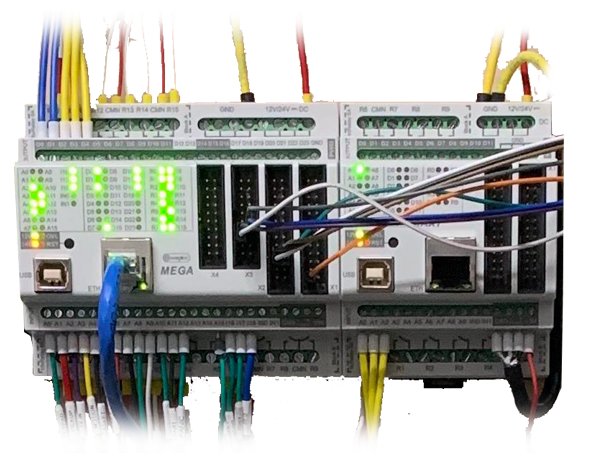
\includegraphics[height=6cm,width=8.5cm]{controllinoPd.png}}
\vspace{3mm}

\begin{Large} 
\textit{Rapport de stage \footnote{Rédigé avec \LaTeX{}}} \\ 
\end{Large}
\begin{Large} 
Spécialité : systèmes industriels automatisés.
\end{Large}
\vspace{1mm}
\rule{0.87\textwidth}{2pt}\\ 
\begin{huge}
\textbf{"Automatisation industrielle efficace avec Controllino :développement, optimisation, formation, applications pratiques.\textbf{"}\\}
\end{huge}
\rule{0.87\textwidth}{2pt}\\ \vspace{0.4cm}
\end{center}
\hspace*{2.3cm}\textbf{R\'e{}alis\'e{} par : \hspace{6cm} Encadr\'e{} par :}\\
\hspace*{2.8cm}\emph{TAIDI LAAMIRI Taha} \hspace{5cm} \emph{Mr. FETTAKA Jalal}\\
\hspace*{2.8cm} \hspace{9.35cm} \emph{Mr. MOULAY HICHAM CHBOUKI}\\

\vspace{0.8cm}
\begin{center}
\textit{Ann\'e{}e universitaire : 2023/2024}
\end{center}
\end{titlepage}
\newpage
%Remerciements--------------------------------------------------------------------
\thispagestyle{empty}
\loadgeometry{2}
\begin{center}
\begin{Huge}
\textcolor{cyan}{\textit{Remerciements}}
\end{Huge}
\end{center}\vspace{2cm}

\newpage
%DÉDICACES-------------------------------------------------------------------------
\thispagestyle{empty}
\begin{center}
\begin{Huge}
\textcolor{red}{\textbf{D\'E{}DICACES}}\\ \vspace{2cm}
\end{Huge}
\textbf{Je dédie ce modeste travail à :}\\
\textbf{M}es chers parents pour leur soutien et leur encouragement durant toute\\
la période de mes études,\\
\textbf{M}a chère sœur,\\
\textbf{M}es frères,\\
\textbf{M}a grande famille,\\
\textbf{A} tous les étudiants de la filière ``systèmes industriels automatisés'',\\
\textbf{A}insi qu’à tous mes amis et collègues sans exception.\\
\end{center}

\newpage
%Avant-propos------------------------------------------------------------------
\thispagestyle{empty}
\begin{center}
\begin{Huge}
\textcolor{red}{\textbf{Avant-propos}}\\
\vspace{2cm}
\end{Huge}
\end{center}
\textbf{Nom et Prénom :}\\
\begin{center}
    TAIDI LAAMIRI Taha, stagiaire en première année, niveau technicien spécialisé en Systèmes Industriels Automatisés à l'Institut de Formation aux Métiers de l'Industrie Automobile de Tanger Free Zone.\\
\end{center}
\textbf{Organisme d'accueil :}\\
\begin{center}
    RNC VALLEY\\
\end{center}
\textbf{Adresse :}\\
\begin{center}
    XXXXXXXX\\
\end{center}
\textbf{Téléphone :}\\
\begin{center}
    +212 600-000000\\
\end{center}
\textbf{Site Web :}\\
\begin{center}
    http://www.robotisames.com/pro/\\
\end{center}
\textbf{Encadrant du projet dans l'entreprise :}\\
\begin{center}
    Mr. MOULAY HICHAM CHBOUKI\\
\end{center}
\textbf{Encadrant pédagogique à l'IFMIA :}\\
\begin{center}
    Mr. Jalal FETTAKA\\
\end{center}
\textbf{Période du stage :}\\
\begin{center}
    Date de début : 02 octobre 2023\\
    Date de fin : 8 janvier 2024
\end{center}
%Table de matière--------------------------------------------------------------
\setcounter{page}{1}
\loadgeometry{4}
\tableofcontents

\newpage
%Liste de figure---------------------------------------------------------------
\loadgeometry{4}
\listoffigures
\addcontentsline{toc}{chapter}{Table des figures}
\nopagebreak
\noindent\begin{minipage}{\textwidth}
\listoftables
\addcontentsline{toc}{chapter}{Liste des tableaux}
\end{minipage}
\newpage
%Introduction------------------------------------------------------------------

%Chapitre1--------------------------------------------------------------------------
\loadgeometry{4}
\chapter{\textbf{Controllino}}
\begin{center}
\rotatebox[origin=c]{360}{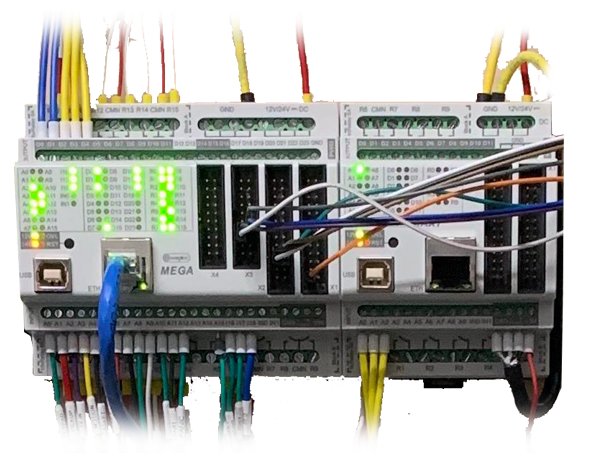
\includegraphics[height=8cm]{controllinoPd.png}}
\captionof{figure}{\texttt{Controllino PLC}}\label{}
\end{center}
\section{Description du Controllino MAXI Power Automation | 100-104-00}
\subsection{Généralités}
Le Controllino MAXI Power Automation est conforme aux normes EN61010-1, EN61010-2-201 et EN61131-2. Il mesure 72x90x62mm et pèse 270g. Il se monte sur un rail DIN standard EN50022 de 35mm.

\subsection{Conditions environnementales}
Le Controllino fonctionne dans des conditions ambiantes de température allant de 0°C à 55°C, avec une humidité relative de 80\% jusqu'à 31°C, déclinant linéairement à 50\% à 55°C. Il supporte un degré de pollution PD2 et peut fonctionner jusqu'à une altitude de 2000m AMSL. Les vibrations sont mesurées à 1,75 mm d'amplitude sinus à des fréquences de 5 à 9 Hz et à 0,5 g d'accélération sinus à des fréquences de 9 à 150 Hz. Il peut être transporté et stocké dans des températures allant de -20°C à +70°C, avec une humidité relative de 10 à 90\% sans condensation, jusqu'à une altitude de 3000m AMSL. Il résiste à des chocs de 15g, avec un demi-sinus de 11ms sur les trois axes.

\subsection{E/S}
Le Controllino fonctionne avec une tension d'alimentation de 24 V. Il possède des entrées/sorties analogiques et numériques, ainsi que des interfaces USB et Ethernet pour la programmation et la communication.

\subsection{Capacités terminales}
Les capacités des borniers varient selon l'usage des sorties (relais, numériques, analogiques) et sont spécifiées en fonction du type de connexion.

\subsection{Protection}
Le Controllino est protégé contre les décharges électrostatiques, les surtensions, les surintensités et les courts-circuits.

\subsection{Caractéristiques électriques}
Les caractéristiques électriques détaillent les plages de tensions et de courants pour les entrées/sorties ainsi que les niveaux logiques.

\subsection{Signalisation LED}
Des LEDs indiquent l'état de l'alimentation, de la programmation, des entrées/sorties et des relais.

\subsection{Dimensions physiques}
Les dimensions physiques du Controllino sont spécifiées pour une installation facile dans divers environnements.

\subsection{PHYSICAL DIMENSIONS}
\begin{center}
\rotatebox[origin=c]{360}{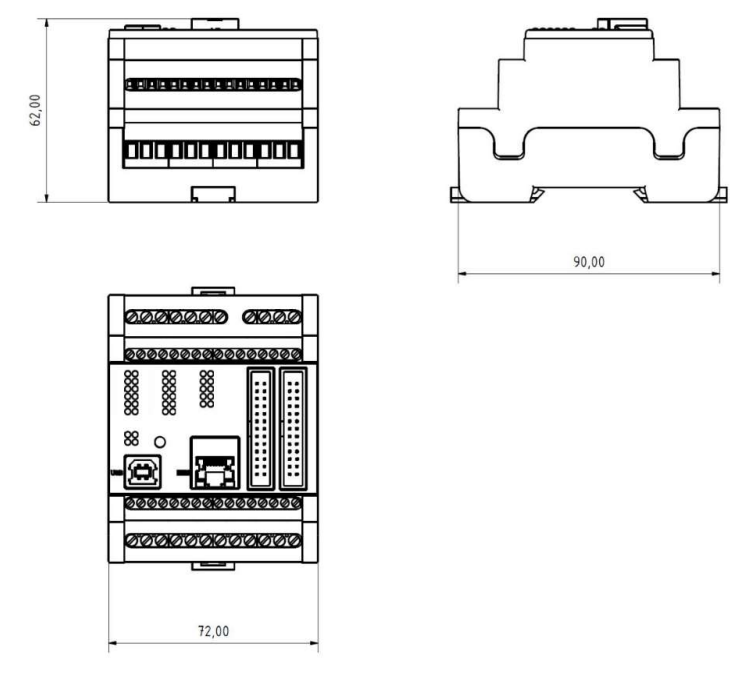
\includegraphics[height=15cm]{PHYSICAL DIMENSIONS controllino maxi power.png}}
\captionof{figure}{\texttt{PHYSICAL DIMENSIONS Controllino maxi power}}\label{}
\end{center}
\subsection{PINOUT}
\begin{center}
\rotatebox[origin=c]{90}{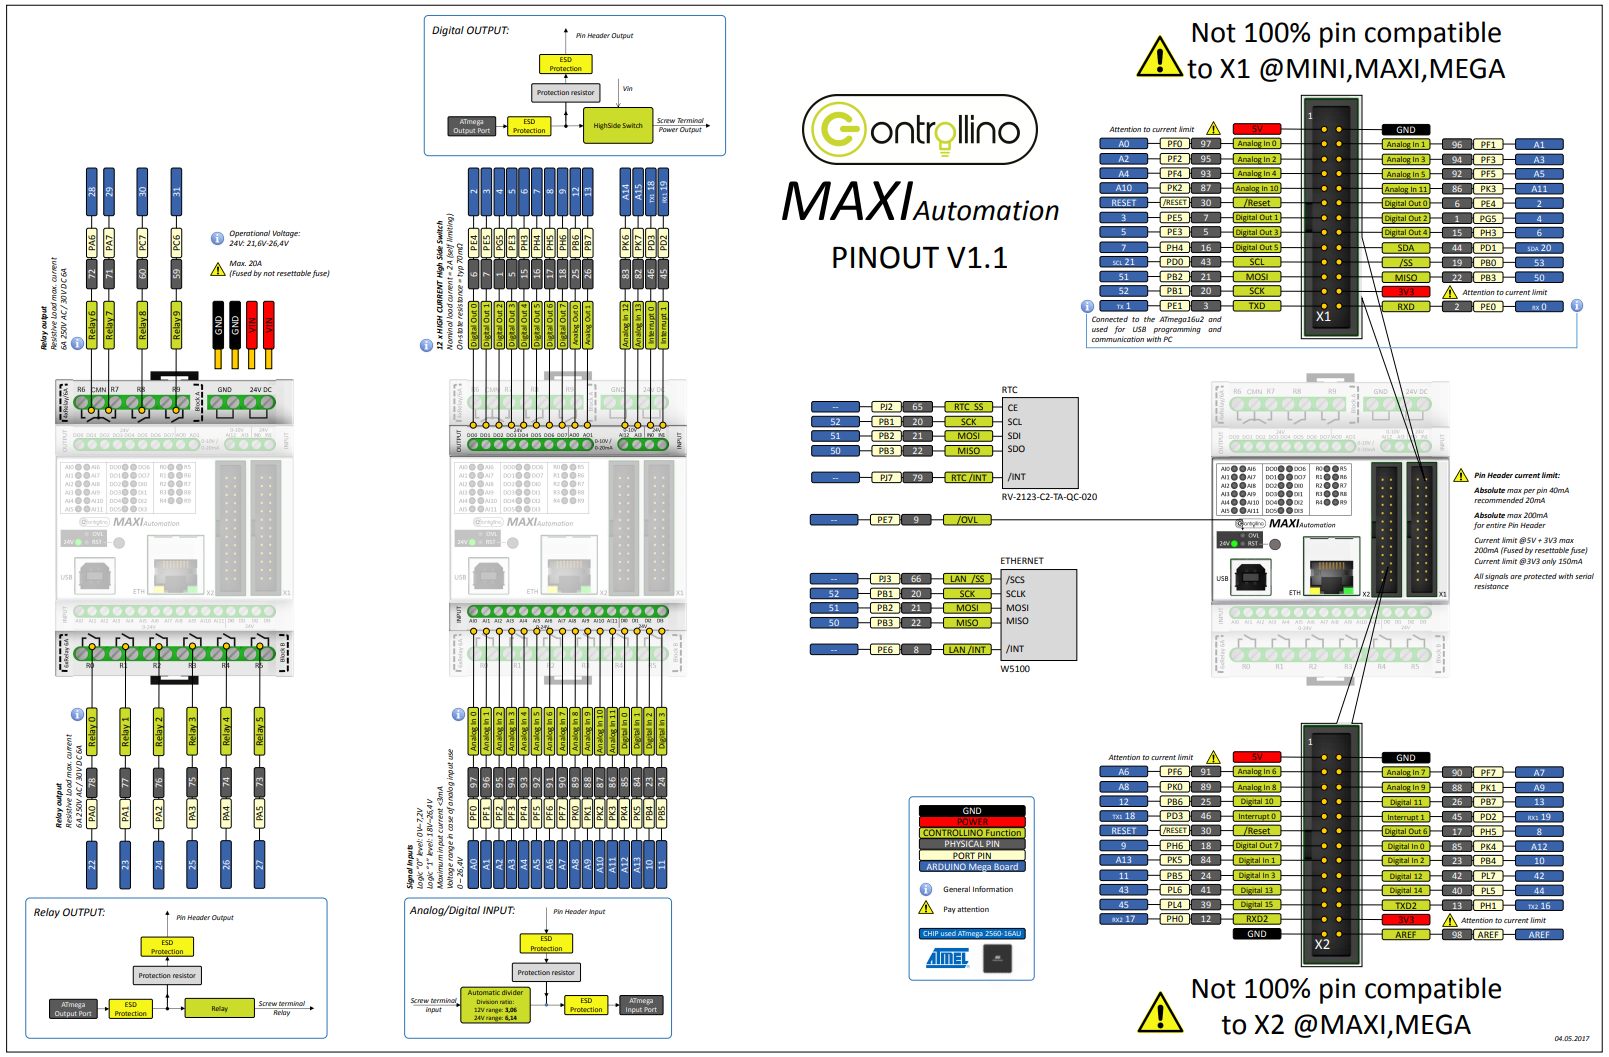
\includegraphics[height=15cm]{controllino maxi power pinout.png}}
\captionof{figure}{\texttt{controllino maxi power Pinout}}\label{}
\end{center}
\newpage
%Chapitre2--------------------------------------------------------------------------
\loadgeometry{4}
\chapter{\textbf{Software setup}}
\section{La mise en place de l'IDE Arduino et de la bibliothèque Controllino}
\subsection{Arduino IDE}
L'Arduino IDE (Environnement de développement intégré) est une application Java polyvalente, libre et compatible avec différentes plateformes, qui trouve ses origines dans Processing. Cette interface sert à la fois d'éditeur de code et de compilateur, facilitant le développement de programmes pour les cartes Arduino. La flexibilité de l'Arduino IDE permet le transfert du firmware et du programme à travers diverses liaisons série telles que RS-232, Bluetooth ou USB, en fonction du module utilisé.\\

Une caractéristique notable de l'Arduino IDE est sa capacité à fonctionner en mode autonome, permettant aux utilisateurs de compiler et de téléverser des programmes sans utiliser l'interface graphique Arduino. Ceci peut être réalisé via l'interface en ligne de commande, offrant ainsi une option plus avancée aux utilisateurs expérimentés.\\

Le langage de programmation employé dans l'Arduino IDE est le C++, compilé à l'aide de avr-g++ et lié à la bibliothèque de développement Arduino. Cette bibliothèque facilite l'utilisation des fonctionnalités de la carte Arduino, y compris ses entrées/sorties. L'adoption du C++ standard simplifie le processus de développement pour toute personne familiarisée avec le langage C ou C++, offrant ainsi une accessibilité accrue à la programmation sur les plates-formes Arduino.\\


\begin{center}

\includegraphics[height=4cm]{arduino_logo.png}
\captionof{figure}{\texttt{Arduino IDE}}\label{}
\end{center}

\subsection{GUIDE DÉTAILLÉ ÉTAPE PAR ÉTAPE POUR L’INSTALLATION la bibliothèque Controllino}

\begin{center}
\includegraphics[height=7cm]{installation d´arduino ide.png}
\captionof{figure}{\texttt{Arduino IDE}}\label{}
\end{center}

Après avoir démarré l’IDE Arduino, naviguez jusqu’à Sketch – Include Library – Manage Libraries\\
(figure 2.3).\\

\begin{center}
\includegraphics[height=10cm]{les bibliothèque manager.png}
\captionof{figure}{\texttt{Navigation vers Library Manager}}\label{}
\end{center}

Dans la fenêtre qui s’ouvre appelée Library Manager écrivez Controllino dans la boîte vide. De la
Sélectionnez Controllino Library et cliquez sur installer \\
(figure 2.4).\\

\begin{center}
\includegraphics[height=7cm]{la bibliothèque de controllino.png}
\captionof{figure}{\texttt{Cherche la bibliothèque de controllino}}\label{}
\end{center}

Le processus automatisé installera Controllino Library sur votre PC. Le succès est montré avec
Étiquette INSTALLÉE à côté du nom de l’article\\
(figure 2.4)\\

\begin{center}
\includegraphics[height=7cm]{Mise en place de la bibliothèque de controllino.png}
\captionof{figure}{\texttt{Mise en place de la bibliothèque de controllino}}\label{}
\end{center}

Naviguer vers le fichier – Préférences \\
(figure 2.6)\\

\begin{center}
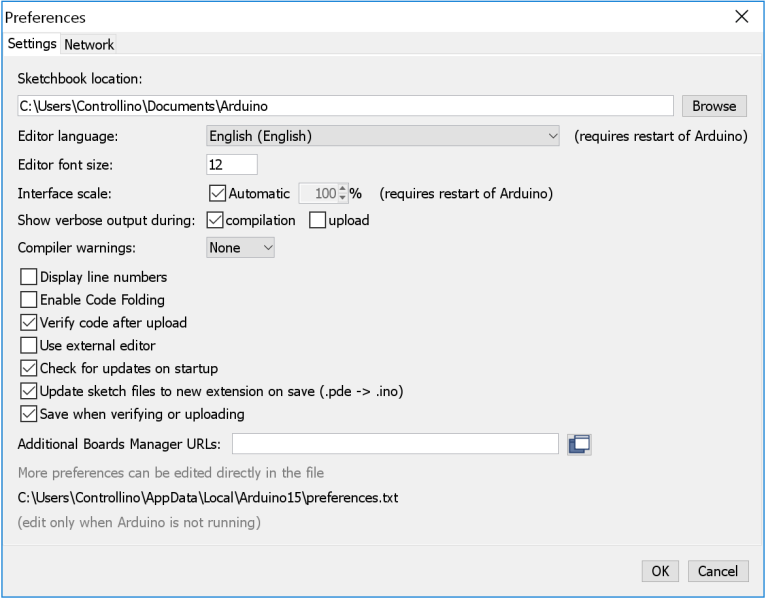
\includegraphics[height=8cm]{Arduino ide préférences.png}
\captionof{figure}{\texttt{Arduino ide préférences}}\label{}
\end{center}

Dans le champ intitulé Additional Boards Manager URLs : coller l’adresse suivante\\ 
(Figure 2.7)\\
et appuyez sur le bouton OK.\\

https://raw.githubusercontent.com/Controllino/ControllinoHardware/master\\
/package\_ControllinoHardware\_index.json
\begin{center}
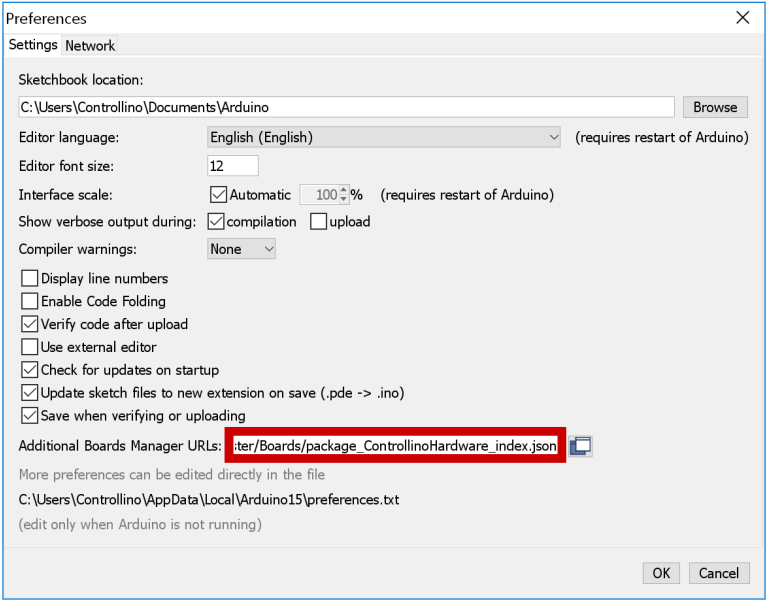
\includegraphics[height=8cm]{ajouter controllino a Arduino ide préférences.png}
\captionof{figure}{\texttt{Ajouter controllino a Arduino ide préférences}}\label{}
\end{center}

Accédez ensuite à Outils – Tableau: «Nom du dernier Carte utilisé» – Carte.
Gestionnaire.\\
(figure 2.8)\\

\begin{center}
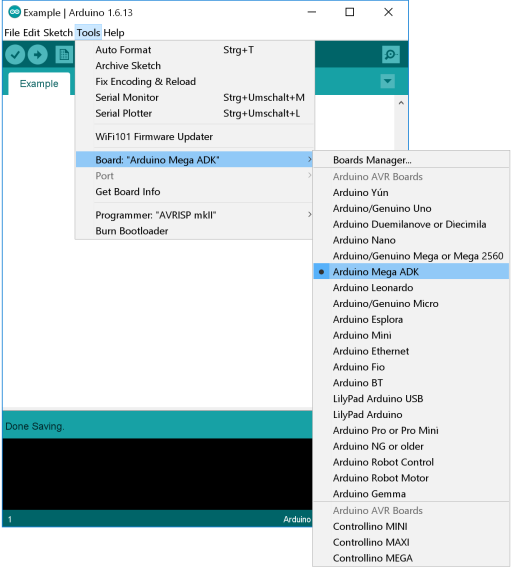
\includegraphics[height=10cm]{gestion des cart arduino.png}
\captionof{figure}{\texttt{Gestion des cart arduino}}\label{}
\end{center}

Dans la fenêtre indiquée, tapez Controllino dans le champ vide.
Les cartes Controllino s’affichent. Cliquez sur le bouton d’installation.\\(figure 2.9)\\

\begin{center}
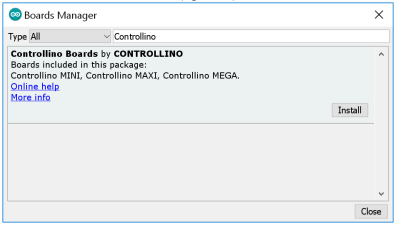
\includegraphics[height=7cm]{la cart de controllino.png}
\captionof{figure}{\texttt{la cart de controllino}}\label{}
\end{center}

Une fois que l’installateur automatisé a terminé le travail, l’élément sera étiqueté\\
INSTALLÉ. (figure 2.10)\\

\begin{center}
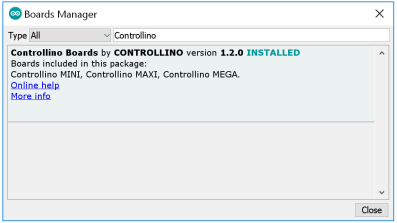
\includegraphics[height=7cm]{ajouter la cart de controllino.png}
\captionof{figure}{\texttt{Ajouter la cart de controllino}}\label{}
\end{center}

Et le package Controllino Hardware vous permettra de voir et de sélectionner les cartes Controllino.\\
(figure 10)\\

\begin{center}
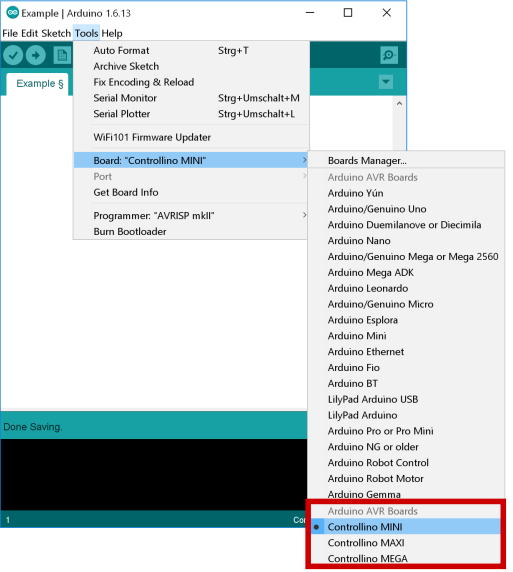
\includegraphics[height=10cm]{choisir la cart de controllino.png}
\captionof{figure}{\texttt{Travier avec la cart de controllino}}\label{}
\end{center}


%Chapitre3--------------------------------------------------------------------------
\loadgeometry{4}
\chapter{\textbf{Trainingsboard }}
\section{PLC4Training}


\section{Instructions techniques pour le tableau de formation PLC V3}
Le tableau de formation PLC peut être équipé d'une alimentation de 12 ou 24 volts en courant continu (CC). Pour cela, utilisez l'alimentation à commutation fournie dans le cadre de la livraison. Respectez les réglementations de sécurité applicables. L'utilisation d'une alimentation non autorisée peut endommager le tableau de formation PLC, le contrôleur ou les dispositifs connectés. Cela annulera la garantie! L'utilisation d'une tension non autorisée peut entraîner des accidents. Le fabricant n'accepte aucune responsabilité pour une utilisation incorrecte!

La LED "Operation" indique une tension d'alimentation suffisante dans la plage de 11,3 à 24,7 volts.

\section*{ÉLÉMENTS DU TABLEAU DE FORMATION PLC}

\begin{itemize}
    \item \textbf{BUZZER}:
    Buzzer\\
    
    \item \textbf{TRANSMETTEUR DE VALEURS ANALOGIQUES}:
    Transmetteur de valeurs analogiques\\
    
    \item \textbf{INTERRUPTEUR D'ENTRÉE DE SIGNAL}:
    8 interrupteurs d'entrée de signal\\
    
    \item \textbf{INTERRUPTEUR ON/OFF À BOUTON-POUSSOIR}:
    Interrupteur ON/OFF à bouton-poussoir\\
    
    \item \textbf{TRANSMETTEUR DE SIGNAL LUMINEUX}:
    Transmetteur de signal lumineux\\
    
    \item \textbf{LED DE SORTIE}:
    8 LEDs de sortie\\
    
    \item \textbf{CODEUR D'IMPULSIONS}:
    Encodeur d'impulsions pour une entrée de comptage rapide I4\\
    
    \item \textbf{CONNECTEUR POUR MODULE D'EXTENSION PLC}:
    Connecteur pour module d'extension PLC\\
    
    \item \textbf{TRANSMETTEUR DE VALEURS ANALOGIQUES AVEC INTERRUPTEUR NUMÉRIQUE/ANALOGIQUE}:
    Transmetteur de valeurs analogiques avec interrupteur numérique/analogique\\
    
    \item \textbf{SURFACE DE MONTAGE POUR CONTROLLINO MAXI OU CONTROLLINO MAXI AUTOMATION}:
    Surface de montage pour Controllino MAXI ou Controllino MAXI Automation\\
    
    \item \textbf{ALIMENTATION}:
    Alimentation de 12 ou 24 volts\\
    
    \item \textbf{SORTIE DE TENSION POUR AFFICHAGE EXTERNE}:
    Sortie de tension pour affichage externe, attention 24V CC\\
    
    \item \textbf{BROCHES D'INTERFACE POUR LA CONNEXION DES MODULES D'INTERFACE}:
    Broches d'interface pour la connexion des modules d'interface\\
    
    \item \textbf{ESPACE RÉSERVÉ POUR LES CARTES DE FORMATION}:
    Espace réservé pour les cartes de formation TR\\
    
    \item \textbf{LED D'OPÉRATION}:
    LED d'opération\\
    
    \item \textbf{INTERRUPTEUR BUZZER ON/OFF}:
    Interrupteur Buzzer ON/OFF\\
    
    \item \textbf{INTERRUPTEUR PULSE ON/OFF}:
    Interrupteur PULSE ON/OFF\\
    
    \item \textbf{INTERRUPTEUR NUMÉRIQUE/ANALOGIQUE}:
    Interrupteur numérique/analogique\\
    
    \item \textbf{TRANSMETTEUR DE VALEURS ANALOGIQUES}:
    Transmetteur de valeurs analogiques pour AI12 et AI13\\
    
    \item \textbf{MONTAGE DU CONTROLLINO}:
    Le Controllino est monté sur un rail DIN.\\
    
    \item \textbf{CONNECTEURS PLC-A ET PLC-B}:
    La connexion électrique entre le Controllino et le tableau de formation PLC se fait via 3 jeux de câbles.\\
    
    \item \textbf{INTERRUPTEURS D'ENTRÉE DE SIGNAL}:
    Les interrupteurs d'entrée de signal peuvent être utilisés pour appliquer un signal numérique.\\
    
    \item \textbf{TRANSMETTEUR DE VALEURS ANALOGIQUES}:
    Avec le transmetteur de valeurs analogiques, une tension d'entrée analogique de 0 à 10 volts peut être appliquée.\\
    
    \item \textbf{INTERRUPTEUR PULSE ON / OFF}:
    Avec l'interrupteur, un générateur d'impulsions peut être connecté en parallèle.\\
    
    \item \textbf{GÉNÉRATEUR D'IMPULSIONS}:
    Le générateur d'impulsions peut être utilisé pour sélectionner le nombre d'impulsions par seconde.\\
    
    \item \textbf{LED DU TRANSMETTEUR DE SIGNAL LUMINEUX}:
    Les 8 LEDs du transmetteur de signal lumineux indiquent l'état de commutation des sorties.\\
    
    \item \textbf{INTERRUPTEUR BUZZER ON / OFF}:
    Avec l'interrupteur Buzzer, un générateur de tonalités peut être activé.\\
    
    \item \textbf{SORTIE DE TENSION POUR AFFICHAGE}:
    Les deux bornes à ressort peuvent être connectées à une tension d'alimentation de 24 volts.\\
    
    \item \textbf{CONNECTEUR POUR LES MODULES D'EXTENSION PLC}:
    Comme il n'existe pas de modules d'extension.\\
    
\end{itemize}
\newpage

\subsection{Training cards Datasheet}
La figure suivante montre la structure schématique de l’écran PLC-Trainingsboard.
\begin{center}
\rotatebox[origin=c]{90}{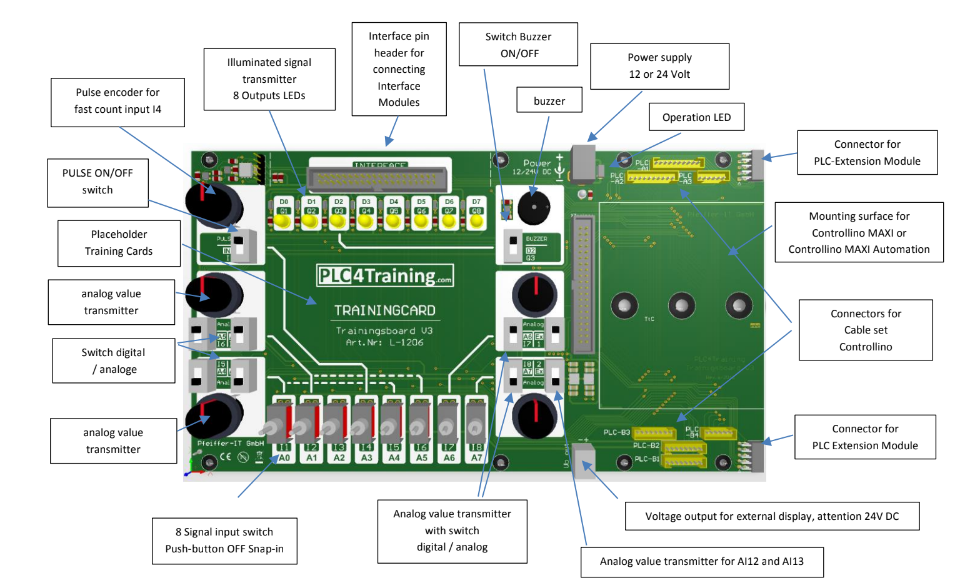
\includegraphics[height=13cm]{Trainingsboard.png}}
\captionof{figure}{\texttt{Training Cart}}\label{}
\end{center}
\subsection{Objectif d'utilisation de PLC4Training}
\begin{center}
\rotatebox[origin=c]{90}{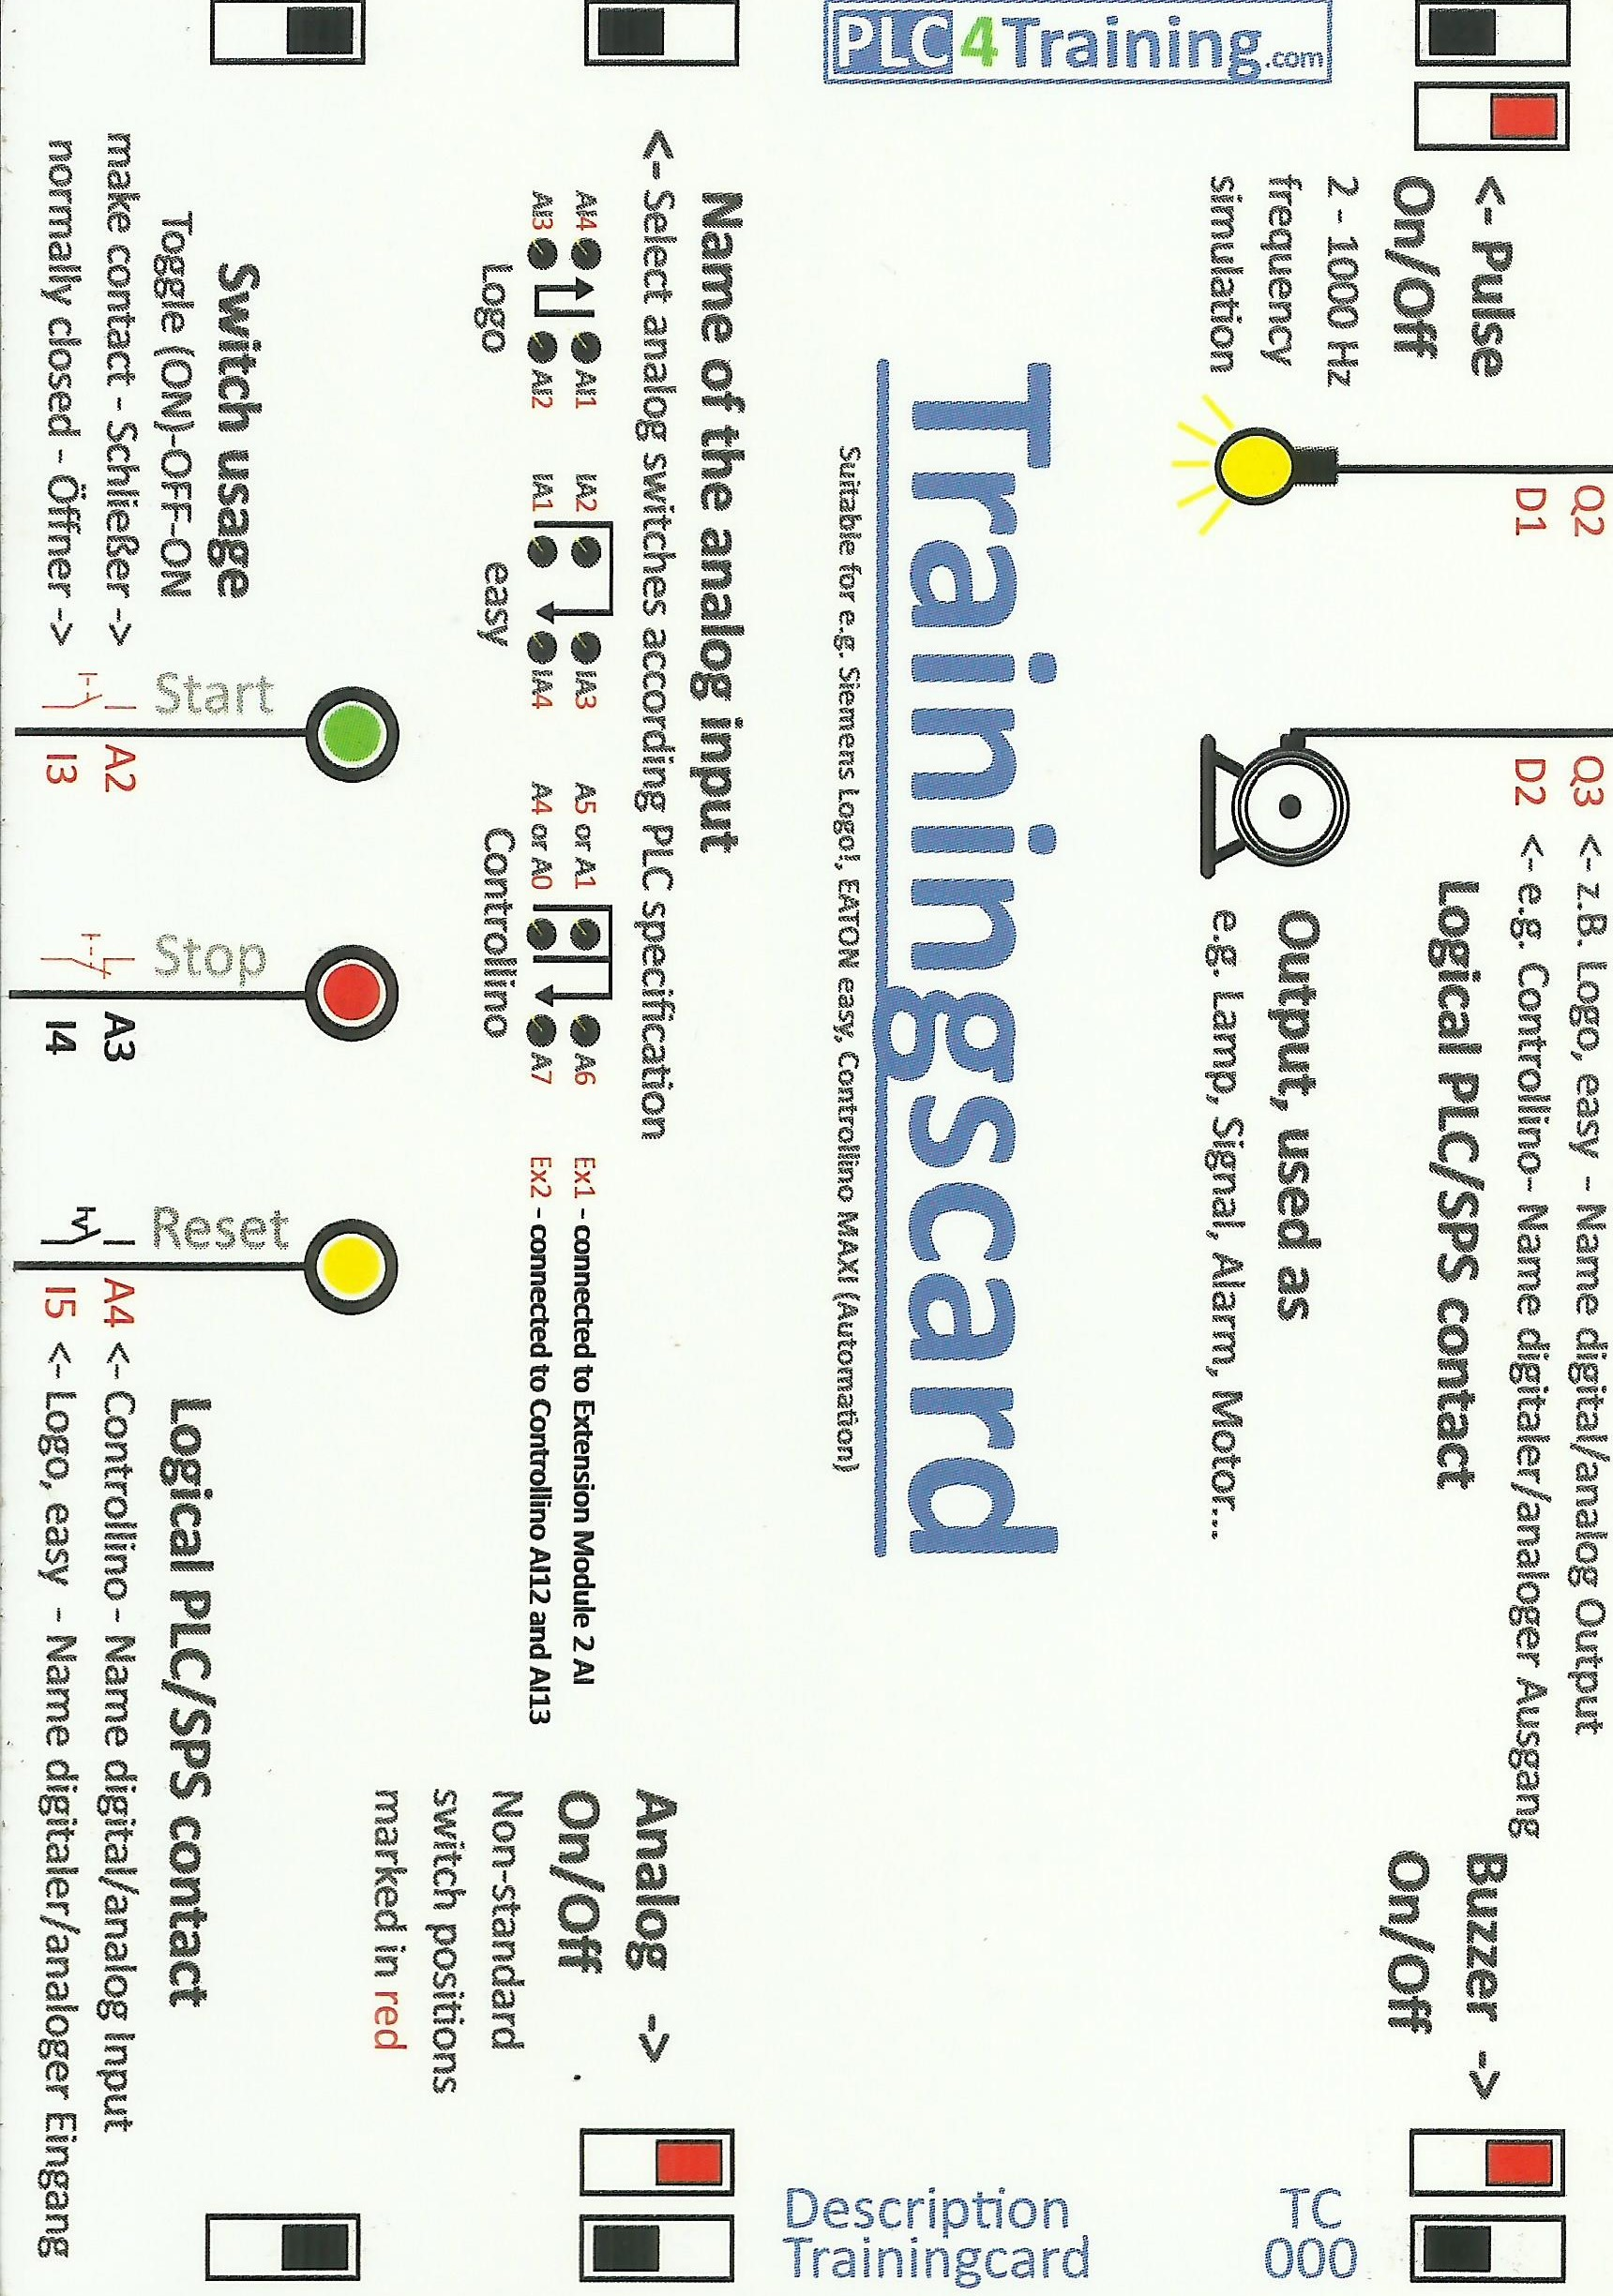
\includegraphics[height=13cm]{000.jpg}}
\captionof{figure}{\texttt{Training Cart}}\label{}
\end{center}
Les formateurs PLC de PLC4Training.com offrent un environnement de formation idéal pour les écoles ou les professionnels de l'éducation. Le PLC-Trainingsboard peut être utilisé à diverses fins, telles que l'enseignement ou la formation scolaire ou professionnelle, la préparation aux examens de la CHAMBRE DE COMMERCE, l'étude, l'apprentissage par la pratique, ainsi que comme dispositif de formation dans les formations pour tester et simuler des solutions. De même, le Controllino Training Kit de Controllino est un kit d’entraînement pour la programmation d’automates programmables. Il est conçu pour être facile à utiliser et convient tant aux débutants qu'aux utilisateurs plus avancés. Compatible avec les automates programmables Controllino, ce kit est parfaitement adapté aux écoles, aux universités, aux entreprises et aux particuliers désireux d'apprendre la programmation d'automates programmables.
\subsection{STRUCTURE DES CARTES DE FORMATION}
\begin{center}
\rotatebox[origin=c]{360}{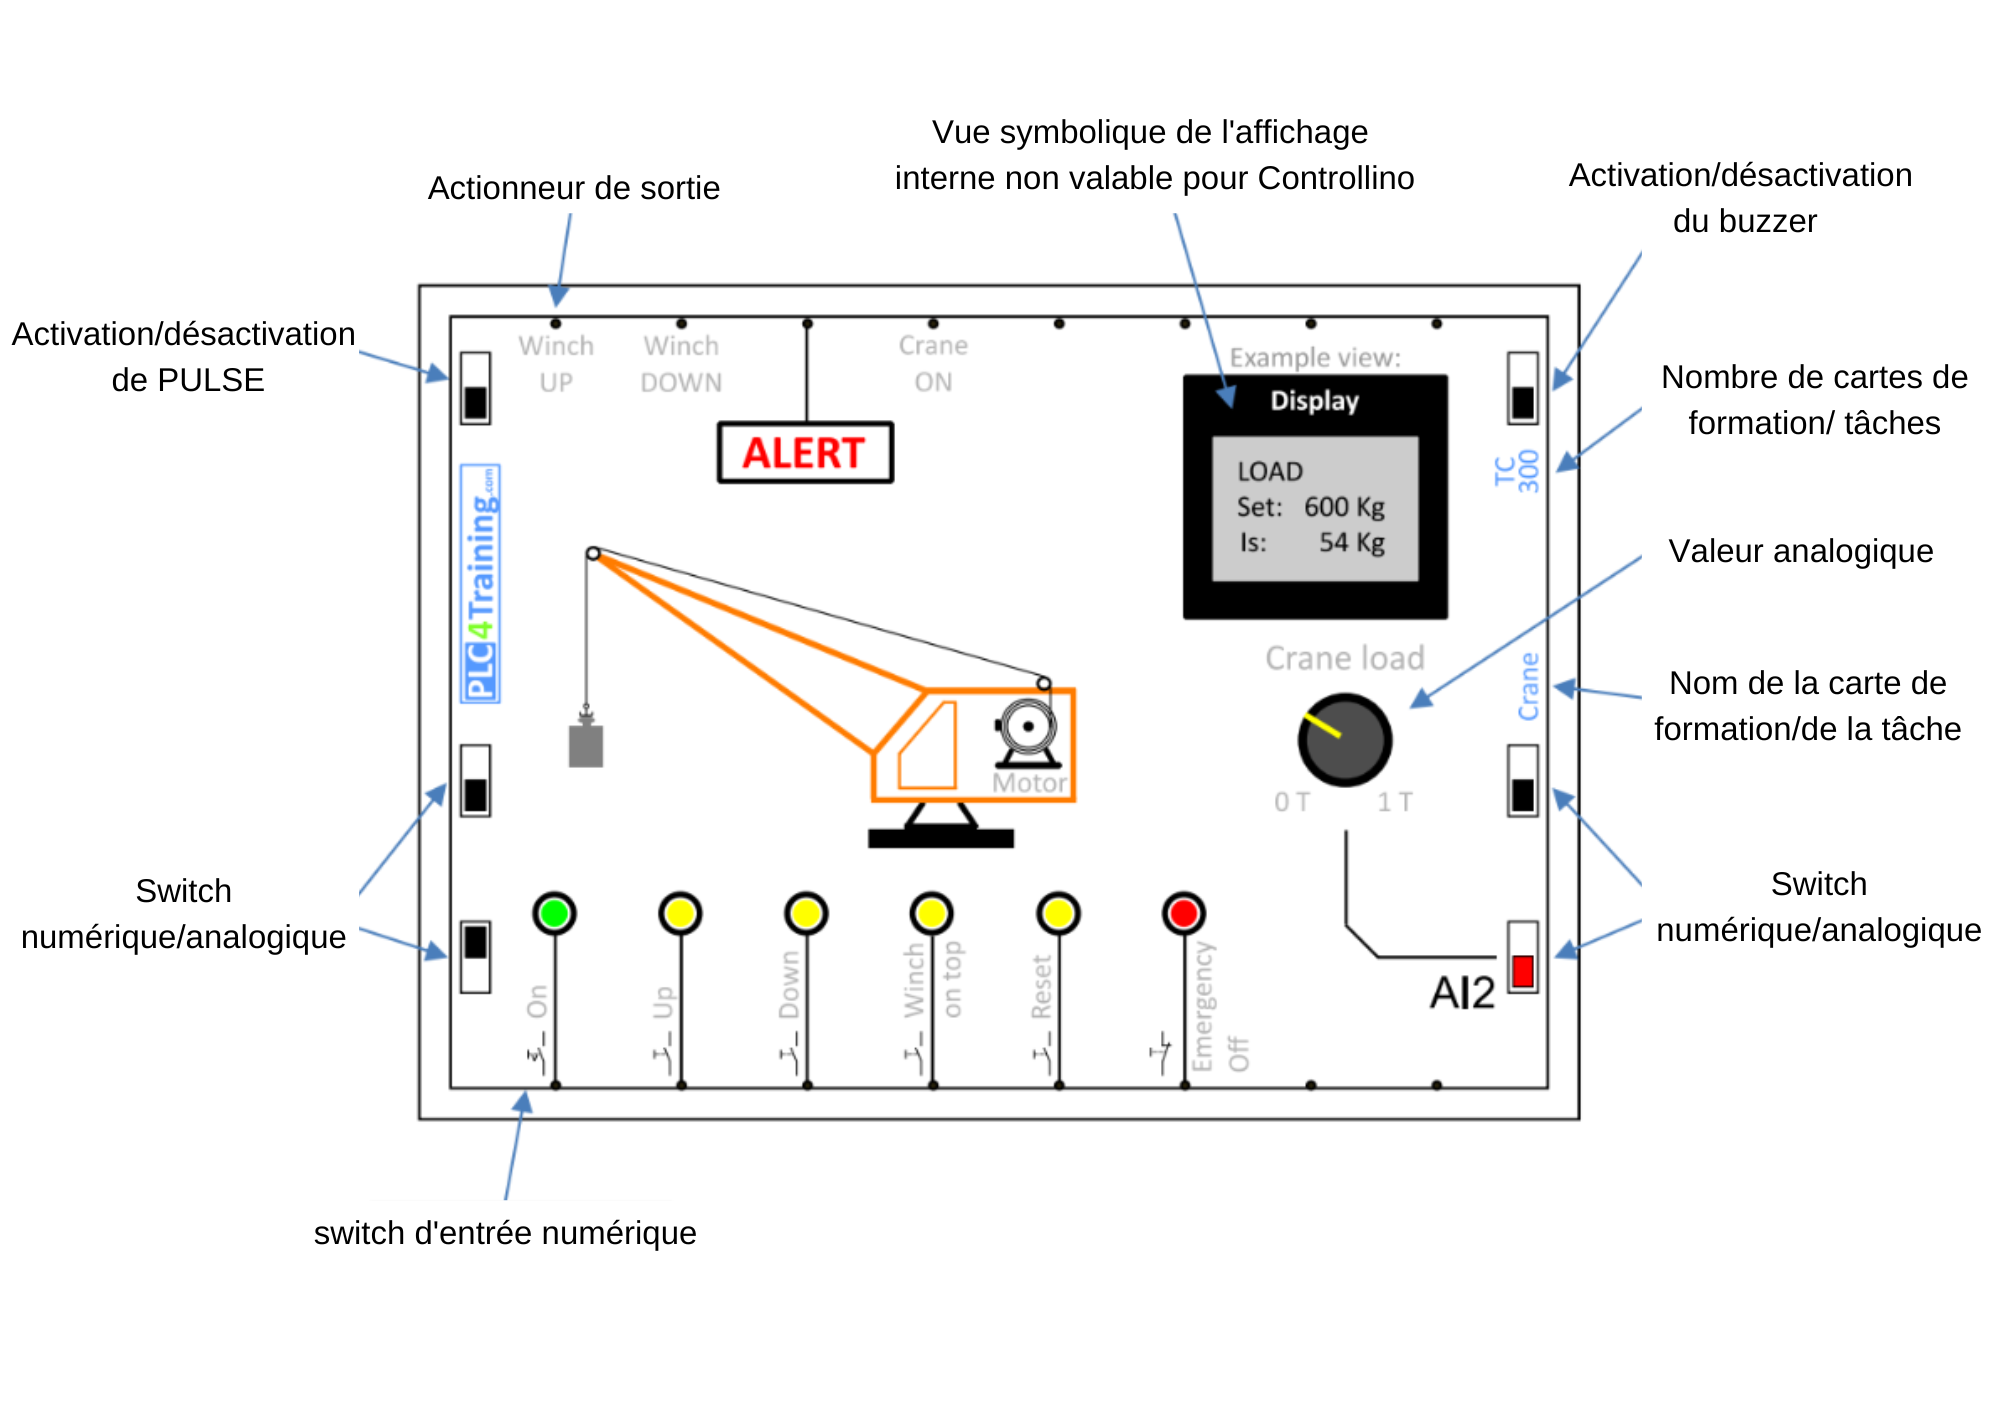
\includegraphics[height=13cm]{STRUCTURE DES CARTES DE FORMATION.png}}
\captionof{figure}{\texttt{STRUCTURE DES CARTES DE FORMATION}}\label{}
\end{center}
\newpage


%Chapitre4--------------------------------------------------------------------------
\loadgeometry{4}
\chapter{\textbf{Controllino-PLC-Sample}}
%TC100--------------------------------------------------------------------------
\section{TC100}

Niveau de difficulté 100 :\\

Les tâches et les cartes de formation du niveau 100 sont très simples. Une esquisse de tâche peut être programmée dans l'IDE Arduino IDE avec quelques lignes de code. Avec les connaissances de base appropriées, une solution peut être élaborée en 45 minutes. Les tâches et les cartes de formation sont marquées comme suit : TC 100, TC 101, TC 102, etc.

%TC100\_ET\_OU\_NON--------------------------------------------------------------------------
\newpage
\subsection{TC100\_ET\_OU\_NON}
\begin{center}
\rotatebox[origin=c]{360}{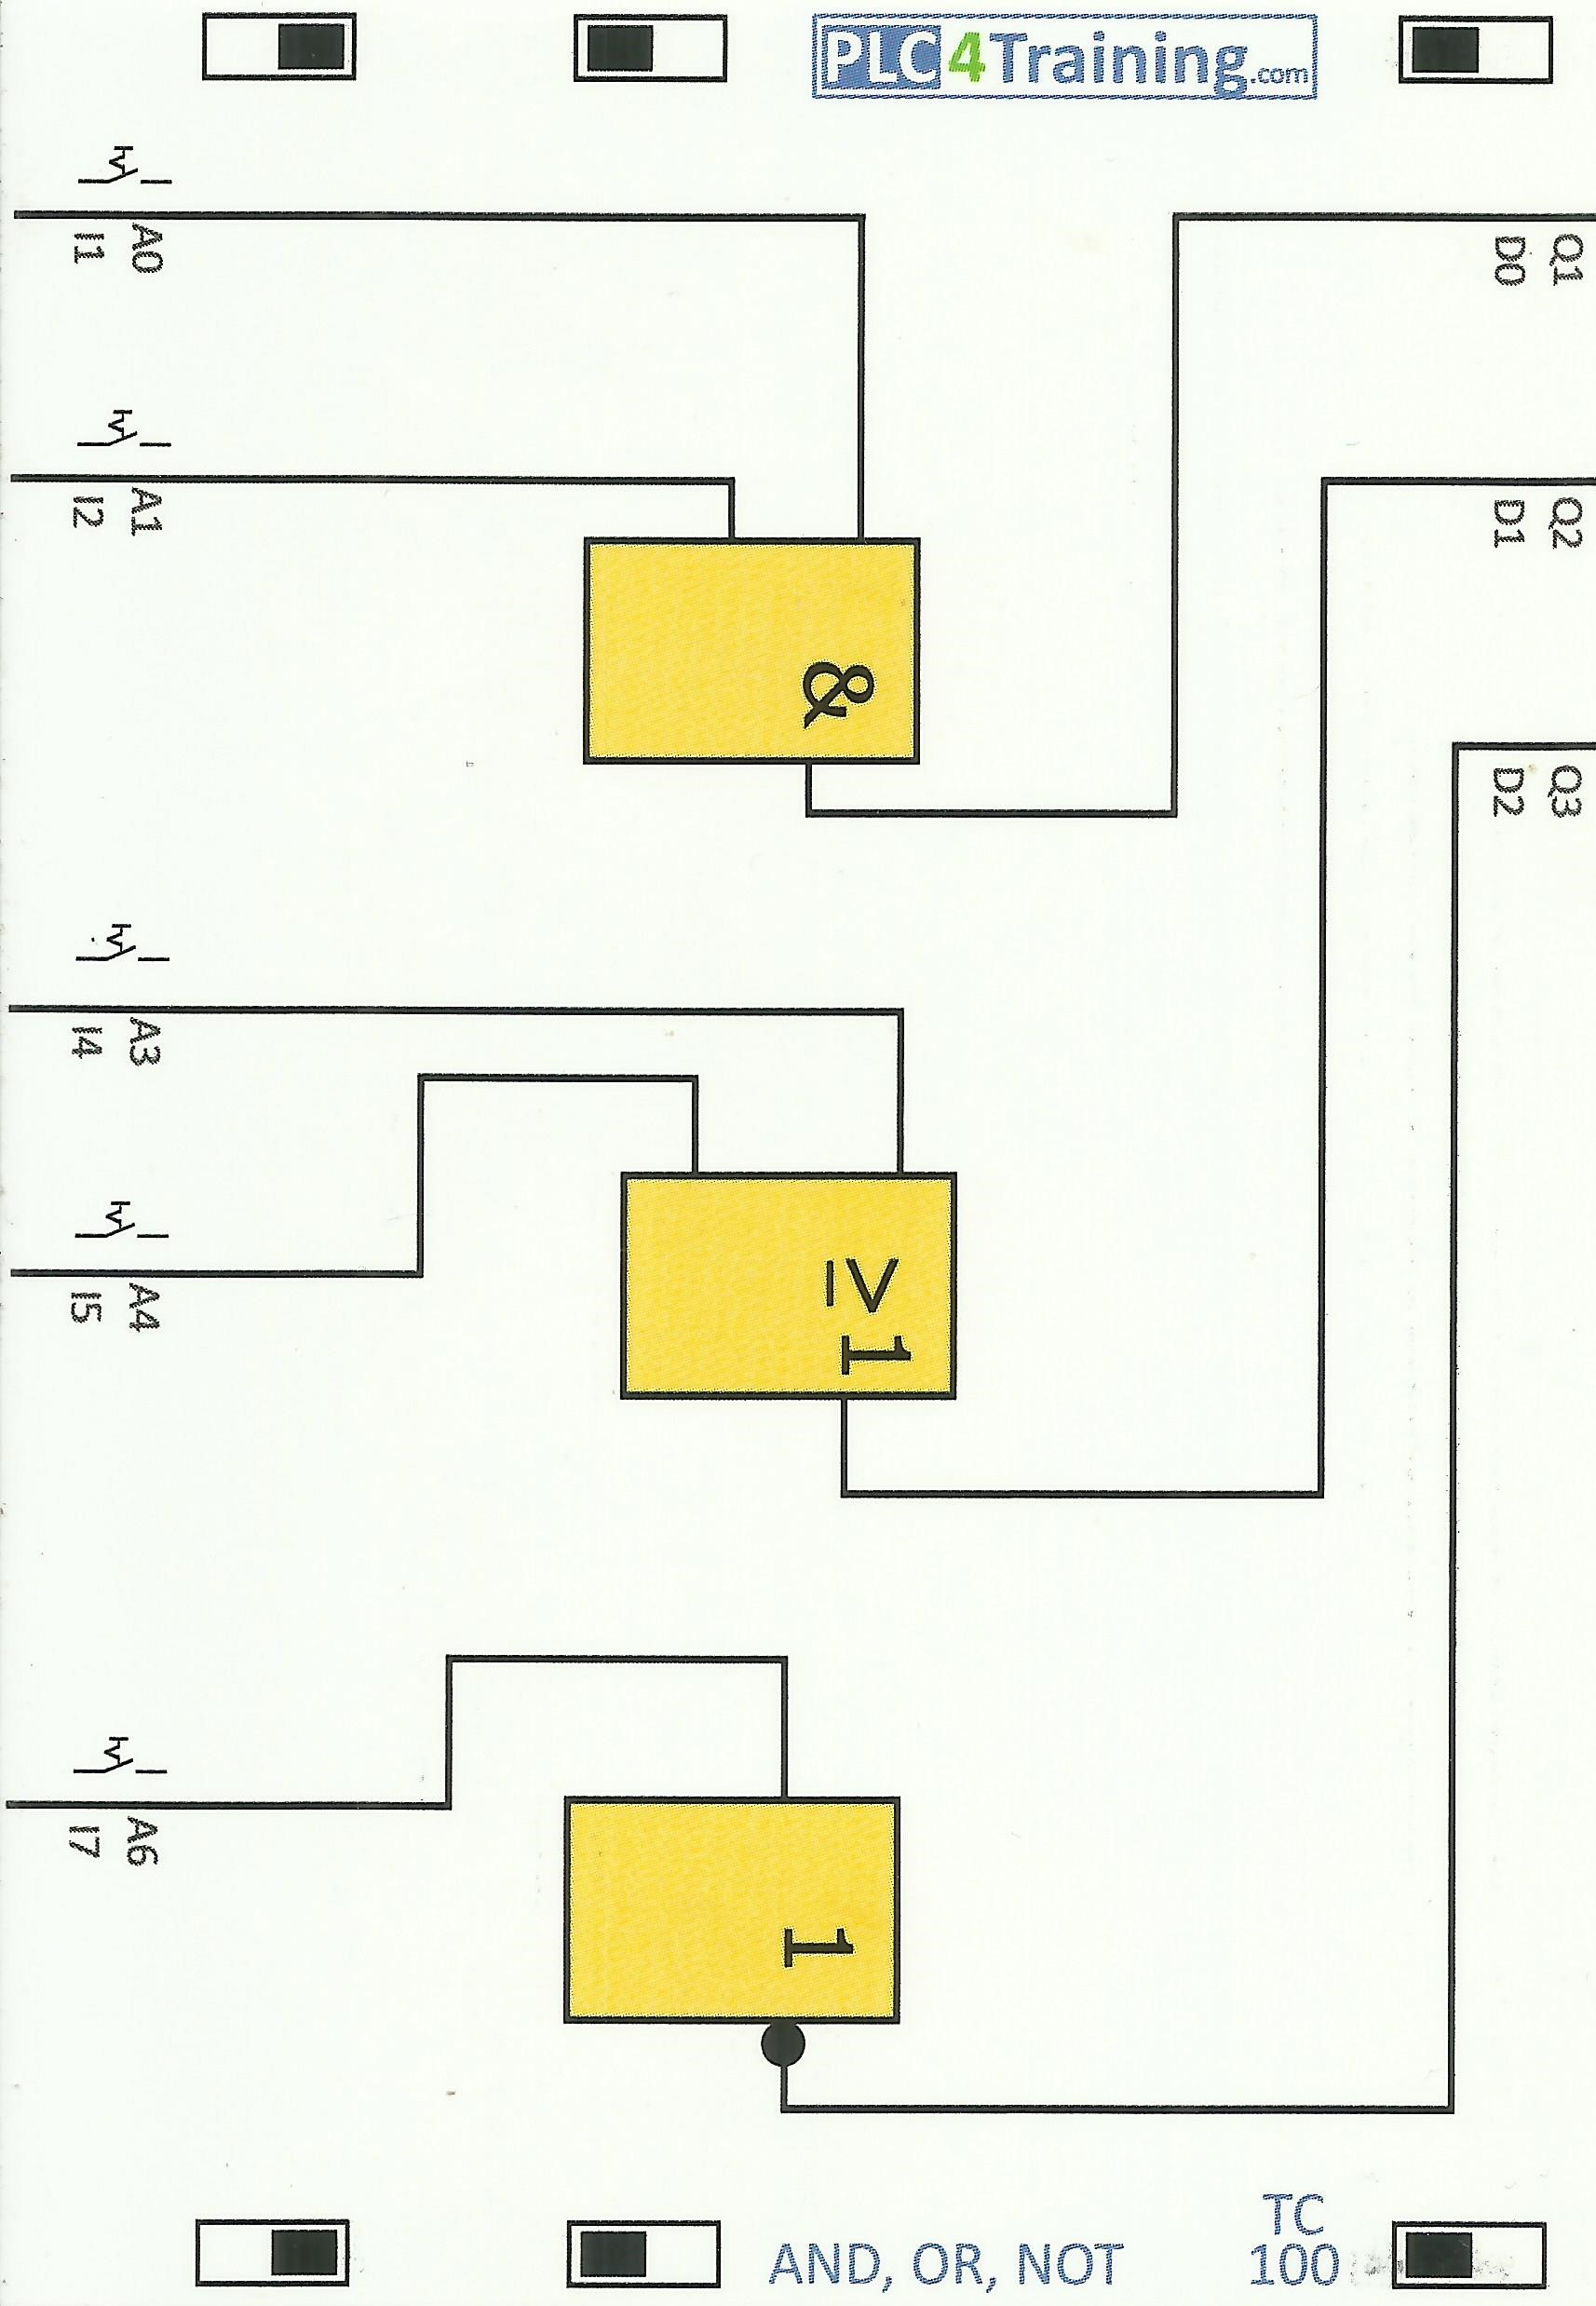
\includegraphics[height=23cm]{100.jpg}}
\captionof{figure}{\texttt{Training Cart 100}}\label{}
\end{center}
\subsubsection{Description du Projet}
Le projet TC 100 a été conçu dans le but de fournir une compréhension approfondie des opérations logiques de base, notamment les opérations AND, OR et  NOT. Chaque tâche de niveau 100 se concentre sur la structure et le fonctionnement de ces opérations logiques, offrant une expérience pratique de programmation pour les débutants dans le domaine.

\subsubsection{Tâches Spécifiques}

\begin{enumerate}
    \item \textbf{Opération AND:} Les tâches liées à l'opération AND impliquent la création d'une structure où les entrées \(A_0\) et \(A_1\) contrôlent la sortie \(D_0\) à l'aide de l'opération logique AND.
    
    \item \textbf{Opération OR:} Les tâches liées à l'opération OR se concentrent sur la configuration où les entrées \(A_3\) et \(A_4\) contrôlent la sortie \(D_1\) à travers l'opération logique OR.
    
    \item \textbf{Opération NOT:} Pour l'opération NOT, la tâche consiste à utiliser l'entrée \(A_6\) pour contrôler la sortie \(D_2\) à l'aide de l'opération logique NOT
\end{enumerate}

\subsubsection{Capteurs/Actionneurs}
Les entrées et sorties du projet sont définies à travers des commutateurs (switches) pour les entrées \(A_0\), \(A_1\), \(A_3\), \(A_4\) et \(A_6\), tandis que les sorties \(D_0\), \(D_1\) et \(D_2\) sont associées à des LEDs. Ces composants permettent une visualisation immédiate des résultats des opérations logiques.

\subsubsection{Code du projet}

\begin{minipage}{0.5\textwidth}
    
\includegraphics[height=3cm]{Code TC100.png}
\end{minipage}%
\begin{minipage}{0.5\textwidth}
    Cliquez sur \href{https://github.com/DexterTaha/Controllino-PLC-Sample/blob/main/TC100/TC100_ET_OU_NON/TC100_ET_OU_NON.ino}{Code} pour obtenir le code.
\end{minipage}

%TC101\_NAND\_NOR\_XOR--------------------------------------------------------------------------
\newpage
\subsection{TC101\_NAND\_NOR\_XOR}
\begin{center}
\rotatebox[origin=c]{360}{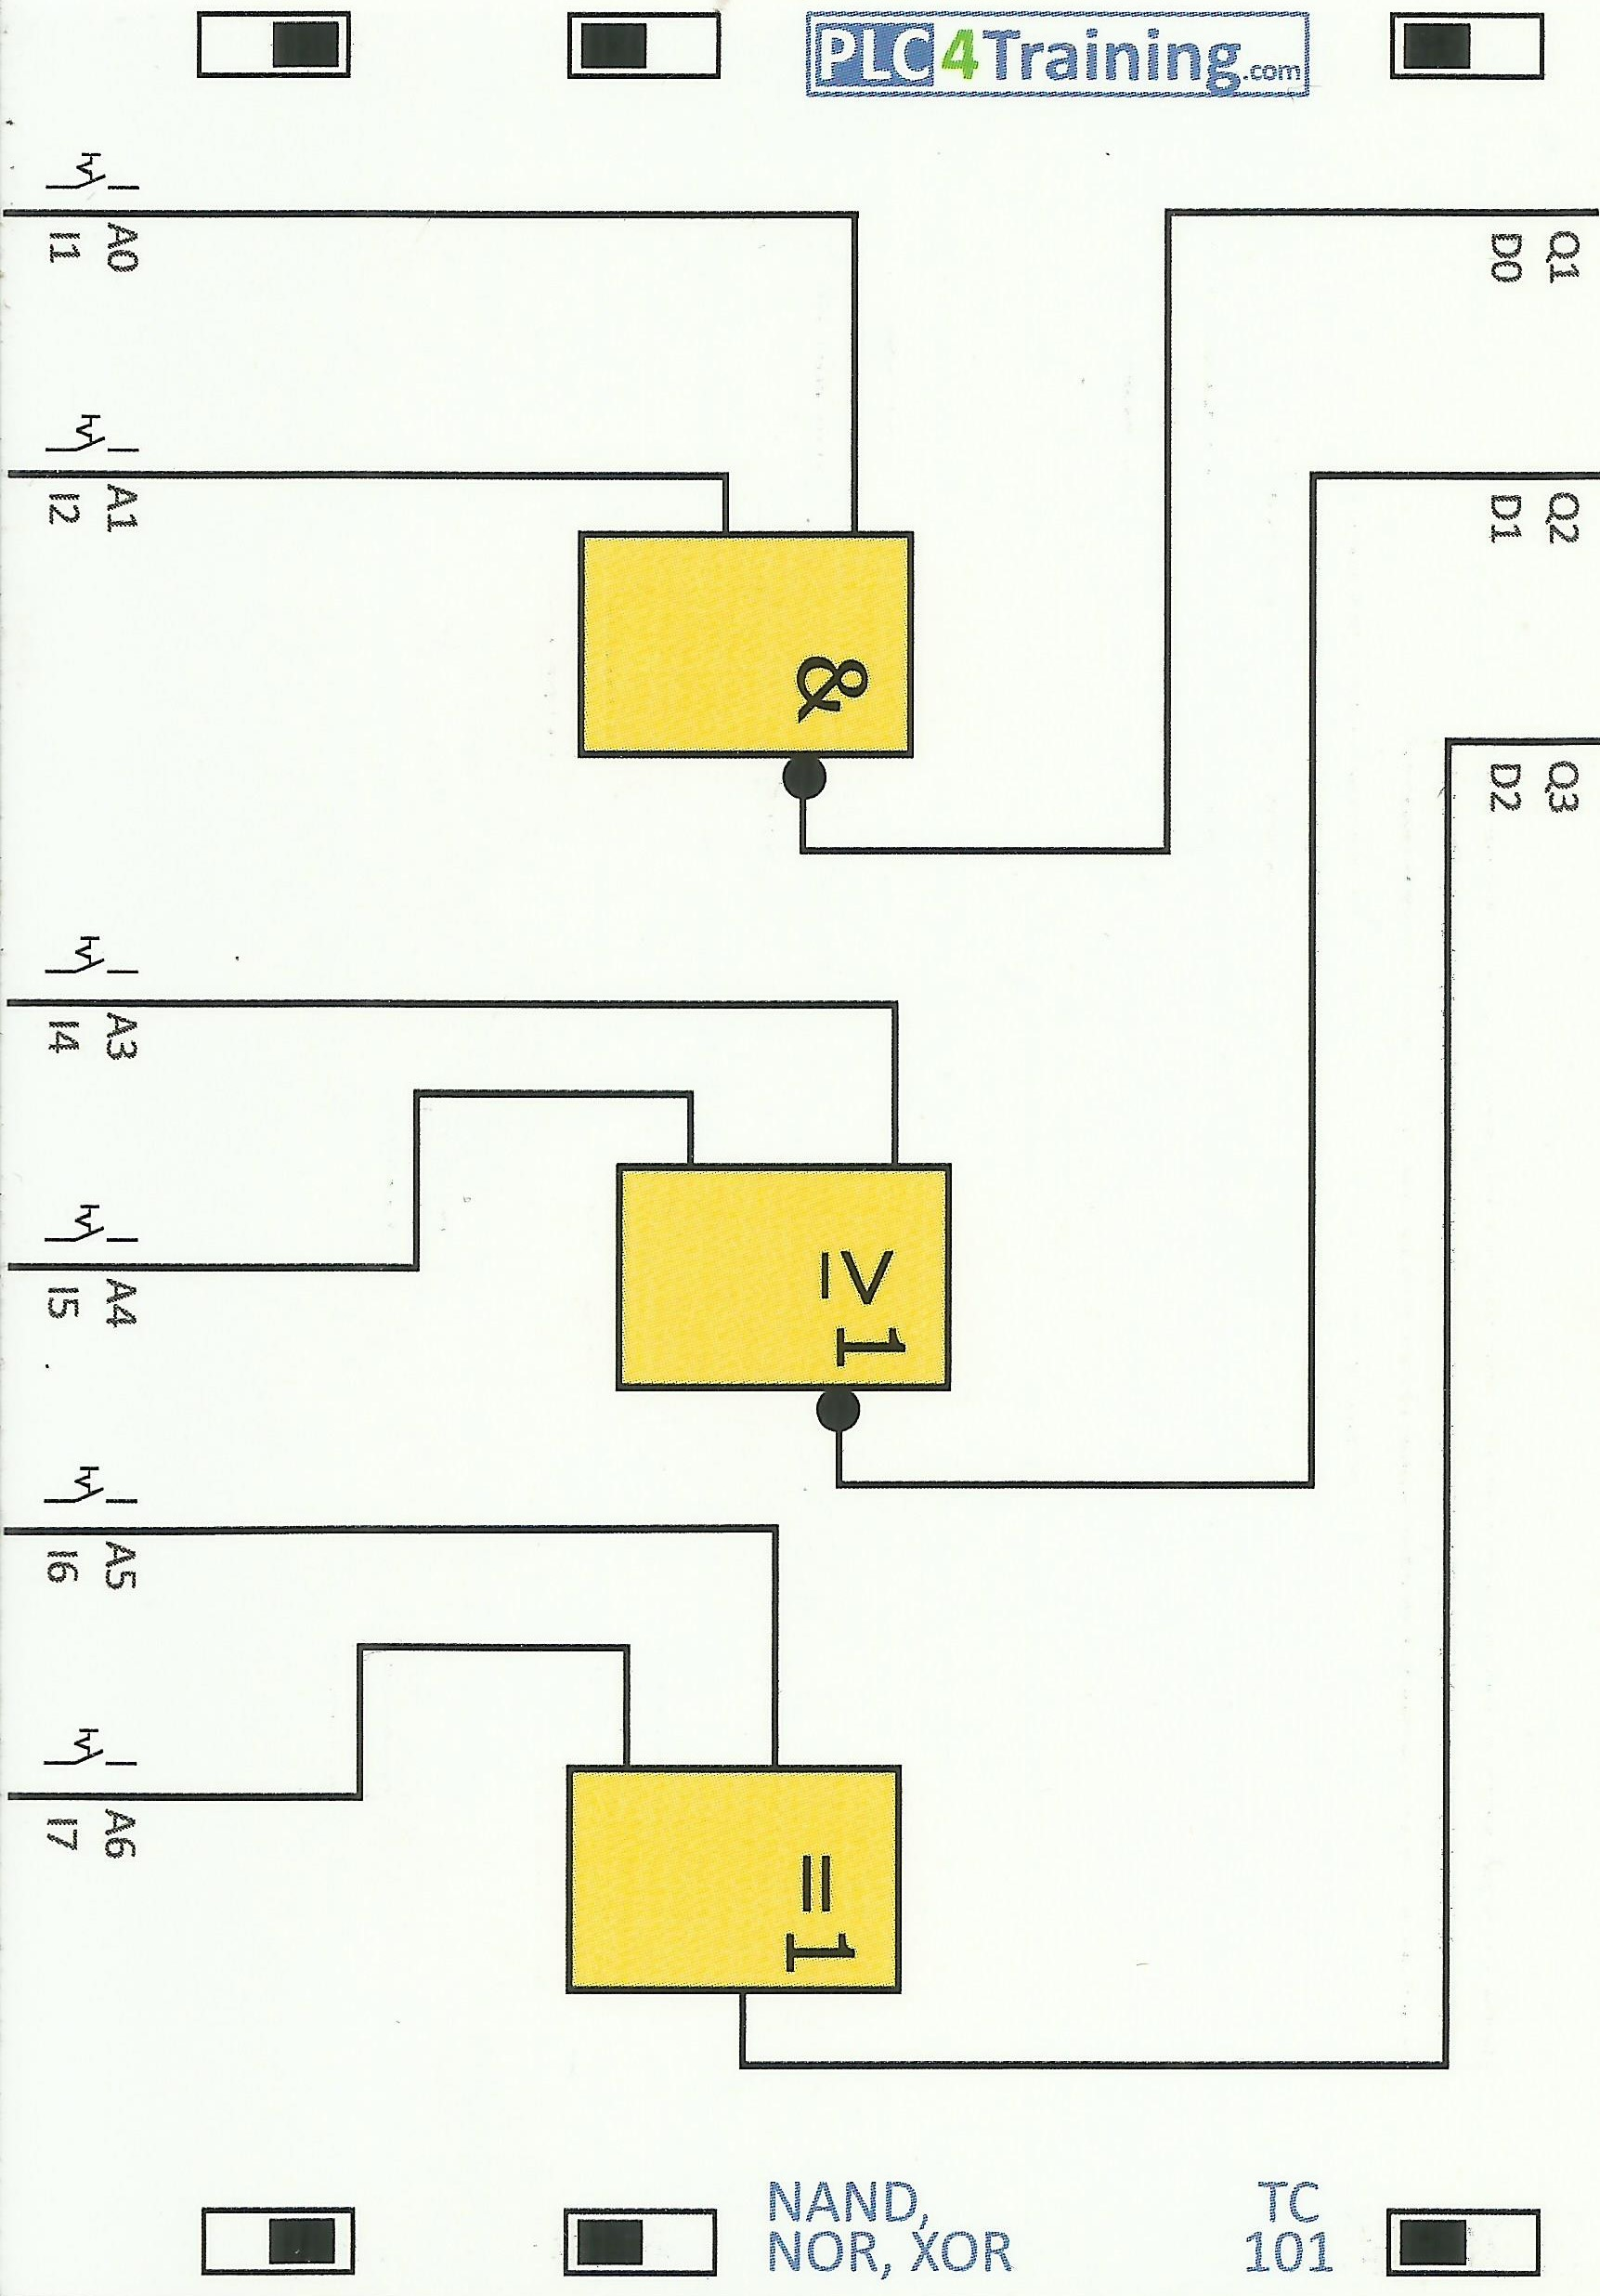
\includegraphics[height=23cm]{101.jpg}}
\captionof{figure}{\texttt{Training Cart 101}}\label{}
\end{center}
\subsubsection{Description du Projet}

Le projet TC 101 a été développé dans le but de présenter et d'approfondir la compréhension des opérations logiques avancées, notamment NAND, NOR et XOR. Chaque tâche de niveau 101 est dédiée à la création et à la compréhension de la structure de ces opérations, fournissant ainsi une expérience pratique pour les participants.

\subsubsection{Tâches Spécifiques}

\begin{enumerate}
   \item \textbf{Opération NAND:} Les tâches associées à l'opération NAND impliquent la configuration où les entrées \(A_0\) et \(A_1\) contrôlent la sortie \(D_0\) à travers l'opération logique NAND.
    
    \item \textbf{Opération NOR:} Les tâches associées à l'opération NOR se concentrent sur la configuration où les entrées \(A_3\) et \(A_4\) contrôlent la sortie \(D_1\) à travers l'opération logique NOR.
    
    \item \textbf{Opération XOR:} Pour l'opération XOR, les tâches consistent à utiliser les entrées \(A_5\) et \(A_6\) pour contrôler la sortie \(D_2\) à travers l'opération logique XOR. 
\end{enumerate}

\subsubsection{Capteurs/Actionneurs}

Les composants du projet incluent des commutateurs pour les entrées \(A_0\), \(A_1\), \(A_3\), \(A_4\), \(A_5\) et \(A_6\), tandis que les sorties \(D_0\), \(D_1\) et \(D_2\) sont associées à des LEDs. Ces éléments permettent une visualisation immédiate des résultats des opérations logiques, renforçant ainsi la compréhension des participants.

\subsubsection{Code du projet}

\begin{minipage}{0.5\textwidth}
    
\includegraphics[height=3cm]{Code TC101.png}
\end{minipage}%
\begin{minipage}{0.5\textwidth}
    Cliquez sur \href{https://github.com/DexterTaha/Controllino-PLC-Sample/blob/main/TC100/TC101_NAND_NOR_XOR/TC101_NAND_NOR_XOR.ino}{Code} pour obtenir le code.
\end{minipage}

%TC102\_Bascule\_RelayTempête--------------------------------------------------------------------------
\newpage
\subsection{TC102\_Bascule\_RelayTempête}
\begin{center}
\rotatebox[origin=c]{360}{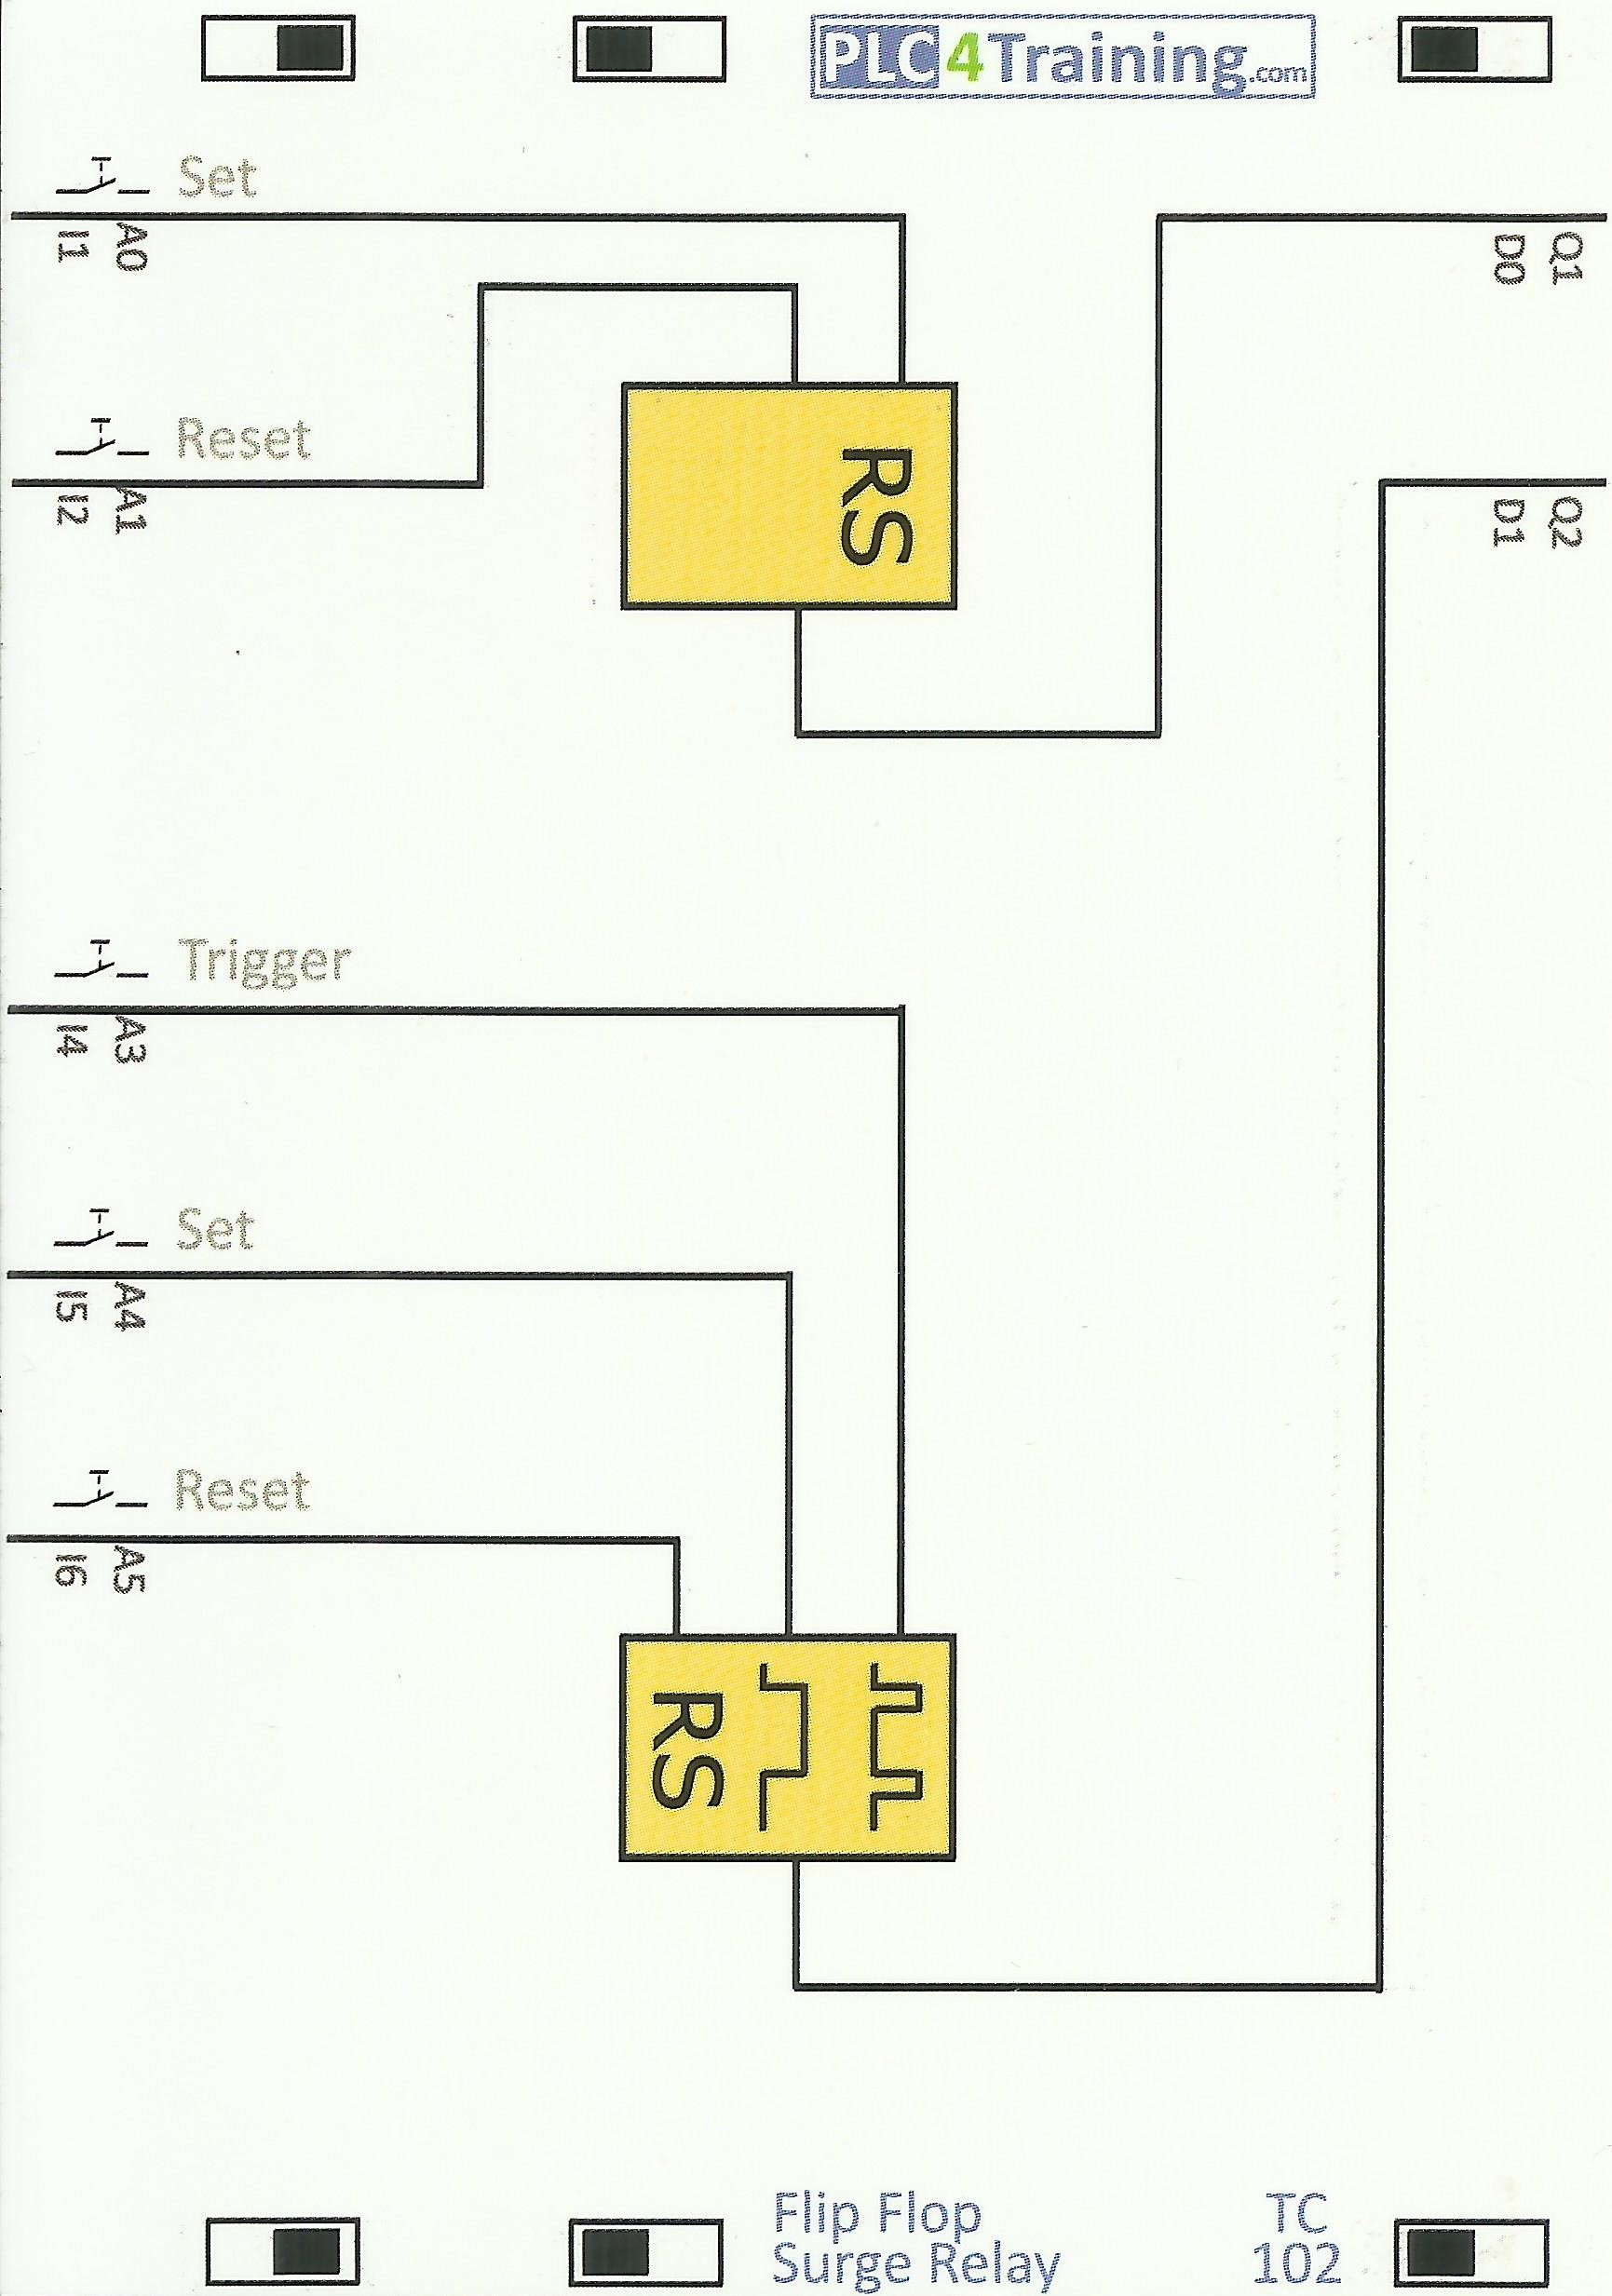
\includegraphics[height=23cm]{102.jpg}}
\captionof{figure}{\texttt{Training Cart 102}}\label{}
\end{center}
\subsubsection{Description du Projet}

Le projet TC 102 a été conçu dans le but d'explorer les concepts avancés de circuits logiques, en mettant l'accent sur le Flip Flop et le Relais d'impulsion (Surge Relay). Chaque tâche de niveau 102 se concentre sur la création de la structure de ces composants, offrant ainsi une expérience pratique et instructive pour les participants.

\subsubsection{Tâches Spécifiques}

\begin{enumerate}
    \item \textbf{Flip Flop:} Les tâches associées au Flip Flop impliquent la configuration où les entrées \(A_0\) et \(A_1\) contrôlent la sortie \(D_0\) en tant que bascule. Le bouton \(A_0\) active la sortie \(D_0\), tandis que le bouton \(A_1\) désactive la sortie \(D_0\).
    
    \item \textbf{Relais d'Impulsion:} La description détaillée du Relais d'Impulsion spécifie que le bouton \(A_3\) doit contrôler le relais d'impulsion et ainsi la sortie \(D_1\). Le bouton \(A_4\) est destiné à régler la sortie de manière sécurisée, tandis que le bouton \(A_5\) est destiné à réinitialiser la sortie de manière sécurisée.
\end{enumerate}

\subsubsection{Capteurs/Actionneurs}

Les composants du projet incluent des boutons pour les entrées \(A_0\), \(A_1\), \(A_3\), \(A_4\) et \(A_5\), tandis que les sorties \(D_0\) et \(D_1\) sont associées à des LEDs. Ces éléments permettent une visualisation immédiate des résultats des opérations, offrant aux participants une expérience concrète dans la manipulation de circuits logiques avancés.

\subsubsection{Code du projet}

\begin{minipage}{0.5\textwidth}
    
\includegraphics[height=3cm]{Code TC102.png}
\end{minipage}%
\begin{minipage}{0.5\textwidth}
    Cliquez sur \href{https://github.com/DexterTaha/Controllino-PLC-Sample/blob/main/TC100/TC102_Bascule_RelayTemp%C3%AAte/TC102_Bascule_RelayTemp%C3%AAte.ino}{Code} pour obtenir le code.
\end{minipage}

%TC103\_Interrupteur\_marche\_arret\_retard--------------------------------------------------------------------------
\newpage
\subsection{TC103\_Interrupteur\_marche\_arret\_retard}
\begin{center}
\rotatebox[origin=c]{360}{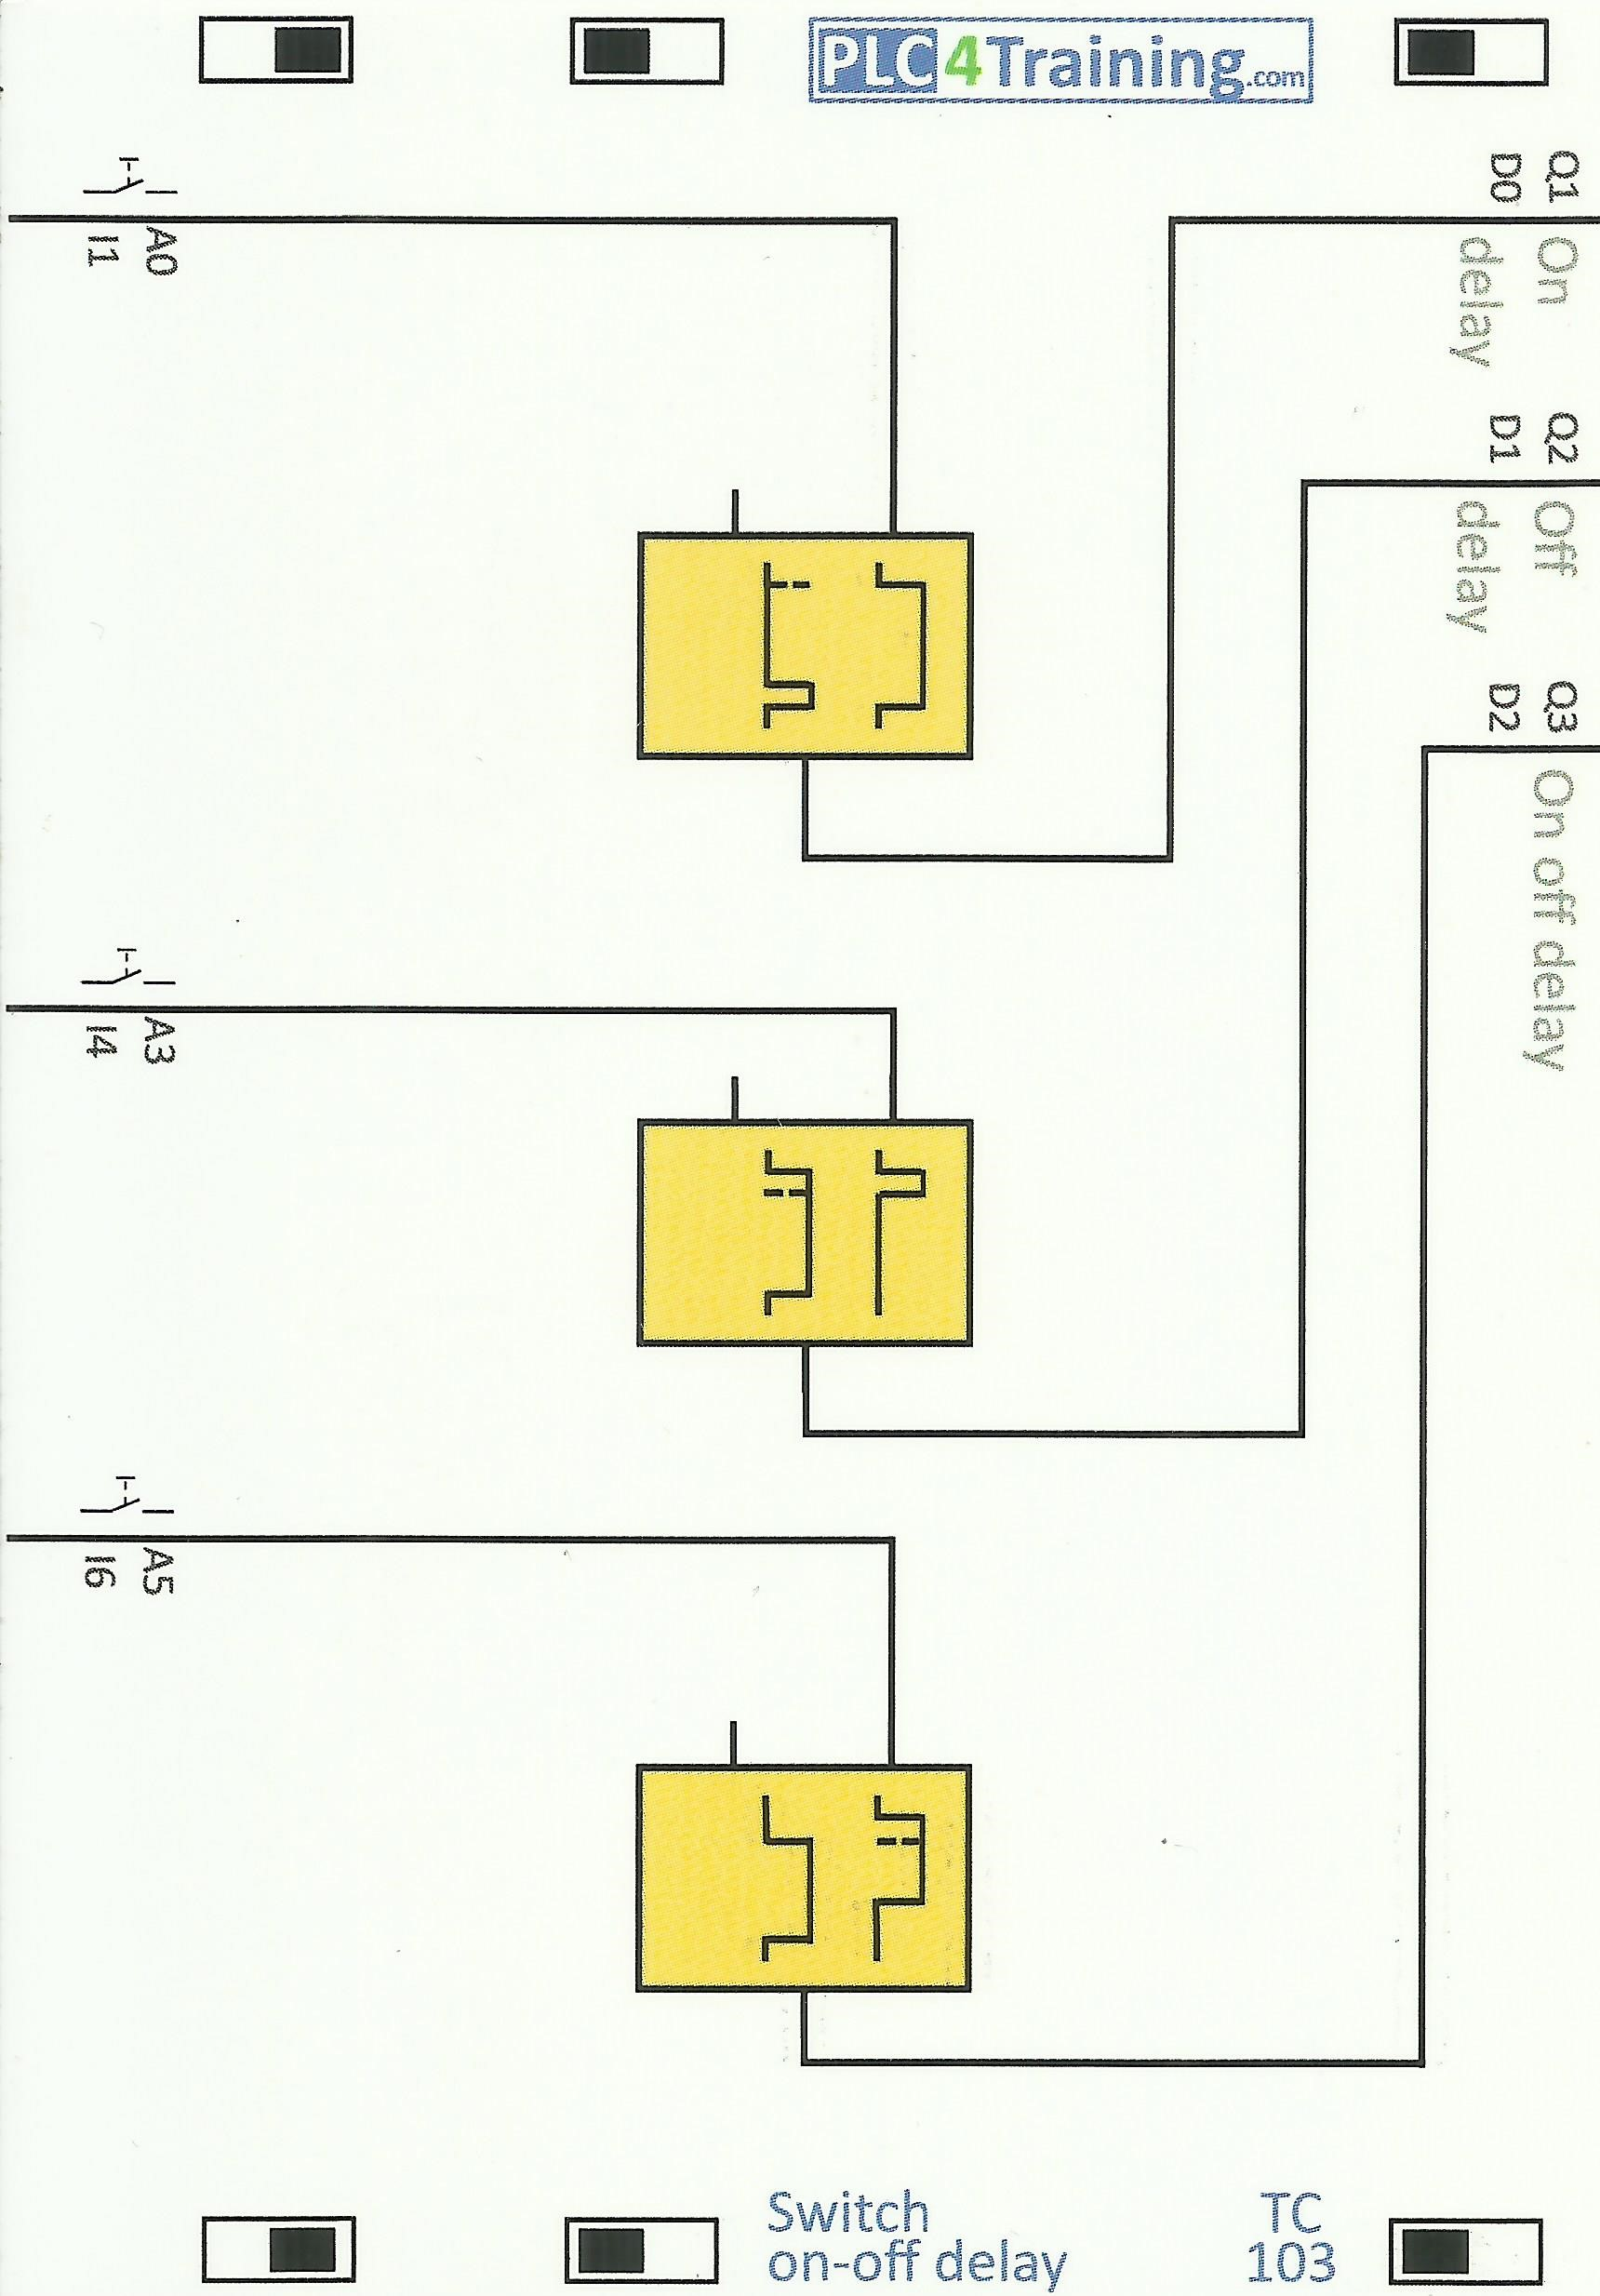
\includegraphics[height=23cm]{103.jpg}}
\captionof{figure}{\texttt{Training Cart 103}}\label{}
\end{center}
\subsubsection{Description du Projet}

Le projet TC 103 a été développé dans le but d'explorer et de comprendre les fonctionnalités avancées des retards de commutation, notamment les retards à l'allumage, à l'extinction et à l'allumage/à l'extinction. Chaque tâche de niveau 103 vise à créer une structure pour ces composants, offrant ainsi une expérience pratique pour les participants.

\subsubsection{Tâches Spécifiques}

\begin{enumerate}
    \item \textbf{Retard à l'Allumage:} La description détaillée du retard à l'allumage spécifie que le bouton \(A_0\) doit contrôler la sortie \(D_0\) avec un retard à l'allumage.
    
    \item \textbf{Retard à l'Extinction:} La tâche associée au retard à l'extinction implique que le bouton \(A_3\) contrôle la sortie \(D_1\) avec un retard à l'extinction.
    
    \item \textbf{Retard à l'Allumage/à l'Extinction:} La description de la tâche pour le retard à l'allumage/à l'extinction indique que le bouton \(A_5\) doit contrôler la sortie \(D_2\).
\end{enumerate}

\subsubsection{Capteurs/Actionneurs}

Les composants du projet incluent des boutons pour les entrées \(A_0\), \(A_3\) et \(A_5\), tandis que les sorties \(D_0\), \(D_1\) et \(D_2\) sont associées à des LEDs. Ces éléments permettent une visualisation immédiate des résultats des retards de commutation, offrant aux participants une expérience pratique dans la manipulation de ces composants avancés.

\subsubsection{Code du projet}

\begin{minipage}{0.5\textwidth}
    
\includegraphics[height=3cm]{Code TC103.png}
\end{minipage}%
\begin{minipage}{0.5\textwidth}
    Cliquez sur \href{https://github.com/DexterTaha/Controllino-PLC-Sample/blob/main/TC100/TC103_Interrupteur_marche_arret_retard/TC103_Interrupteur_marche_arret_retard.ino}{Code} pour obtenir le code.
\end{minipage}

%TC104\_Générateur\_d'impulsions--------------------------------------------------------------------------
\newpage
\subsection{TC104\_Générateur\_d'impulsions}
\begin{center}
\rotatebox[origin=c]{360}{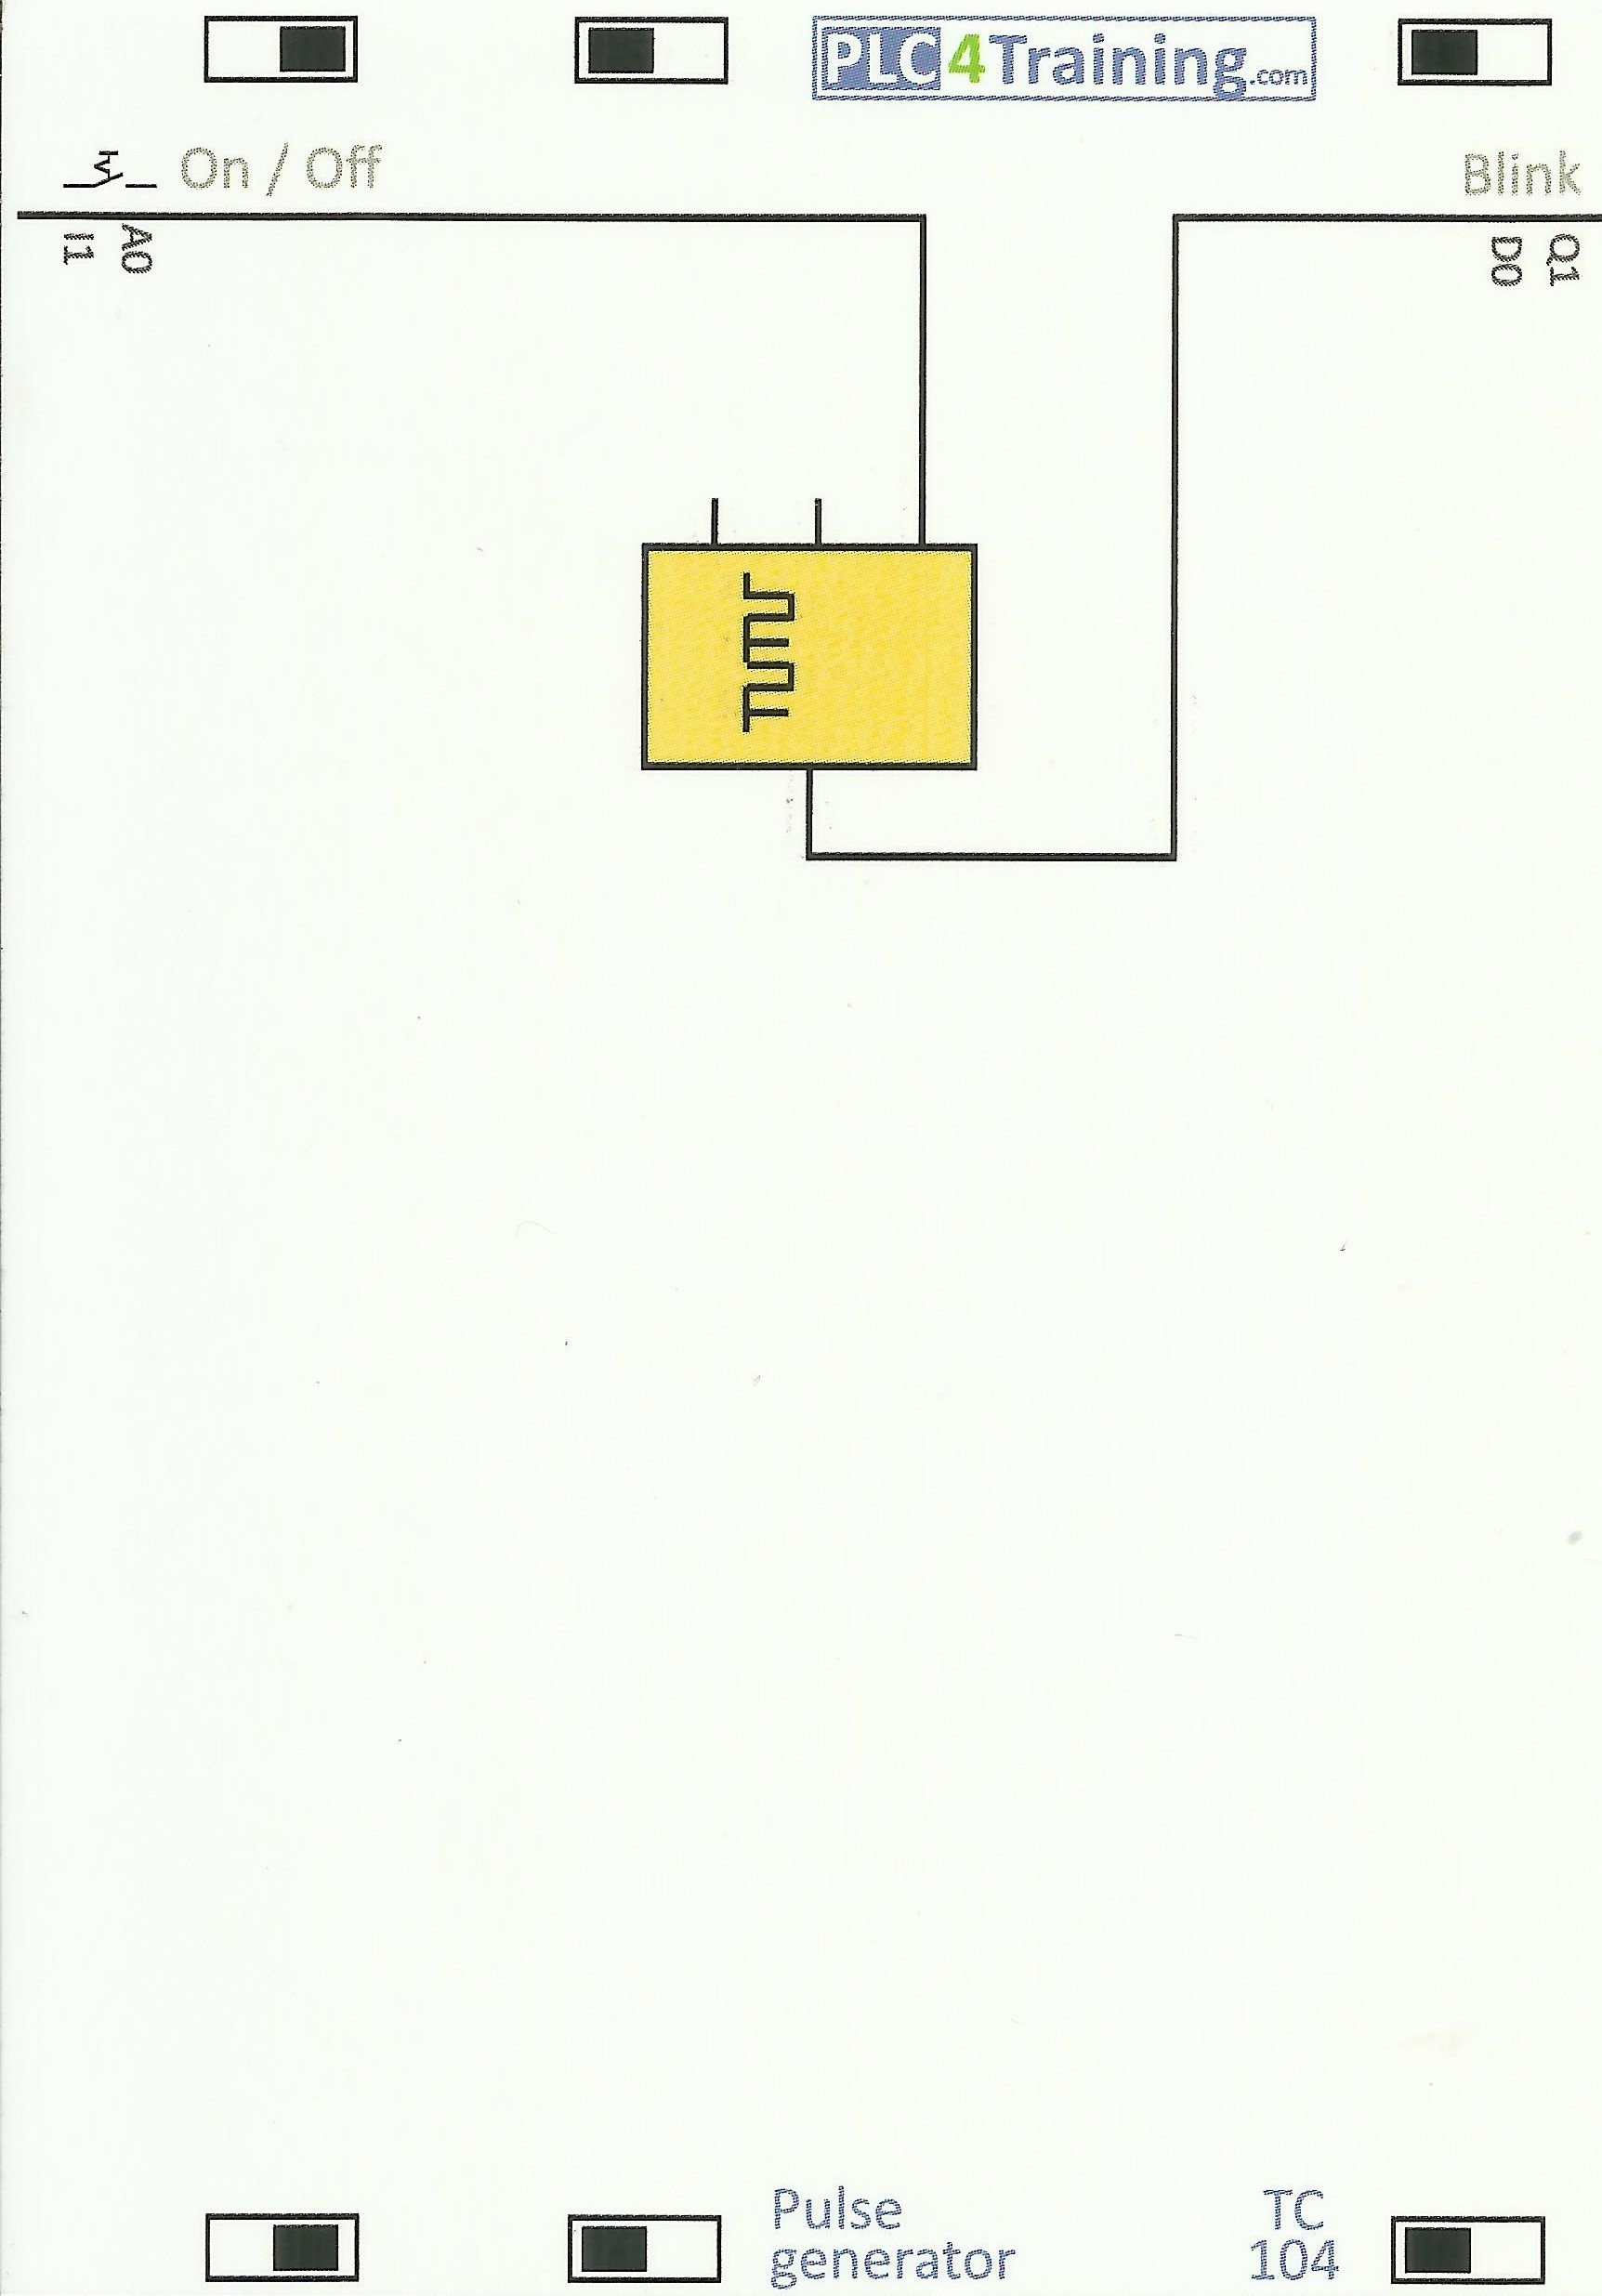
\includegraphics[height=23cm]{104.jpg}}
\captionof{figure}{\texttt{Training Cart 104}}\label{}
\end{center}
\subsubsection{Description du Projet}

Le projet TC 104 a été élaboré dans le but de familiariser les participants avec la structure et le fonctionnement d'un générateur d'impulsions, en mettant l'accent sur la création d'une lumière clignotante. La tâche de niveau 104 vise à fournir une expérience pratique permettant de comprendre la génération d'impulsions, avec une durée d'impulsion et une durée de pause de chaque impulsion fixées à 1 seconde.

\subsubsection{Tâches Spécifiques}

\begin{enumerate}
    \item \textbf{Générateur d'Impulsions:} La description détaillée de la tâche spécifie que le bouton \(A_0\) est utilisé pour activer le générateur d'impulsions, produisant ainsi une lumière clignotante à la sortie \(D_0\). La durée d'impulsion et la durée de pause de chaque impulsion sont définies à 1 seconde.
\end{enumerate}

\subsubsection{Capteurs/Actionneurs}

Les composants du projet incluent un bouton pour l'entrée \(A_0\), tandis que la sortie \(D_0\) est associée à une LED qui clignote. Ces éléments permettent une visualisation immédiate du générateur d'impulsions, offrant aux participants une expérience pratique dans la manipulation de ce composant spécifique.

\subsubsection{Code du projet}

\begin{minipage}{0.5\textwidth}
    
\includegraphics[height=3cm]{Code TC104.png}
\end{minipage}%
\begin{minipage}{0.5\textwidth}
    Cliquez sur \href{https://github.com/DexterTaha/Controllino-PLC-Sample/blob/main/TC100/TC104_G%C3%A9n%C3%A9rateur_d'impulsions/TC104_G%C3%A9n%C3%A9rateur_d'impulsions.ino}{Code} pour obtenir le code.
\end{minipage}

%TC105\_Circuit\_de\_croisement--------------------------------------------------------------------------
\newpage
\subsection{TC105\_Circuit\_de\_croisement}
\begin{center}
\rotatebox[origin=c]{360}{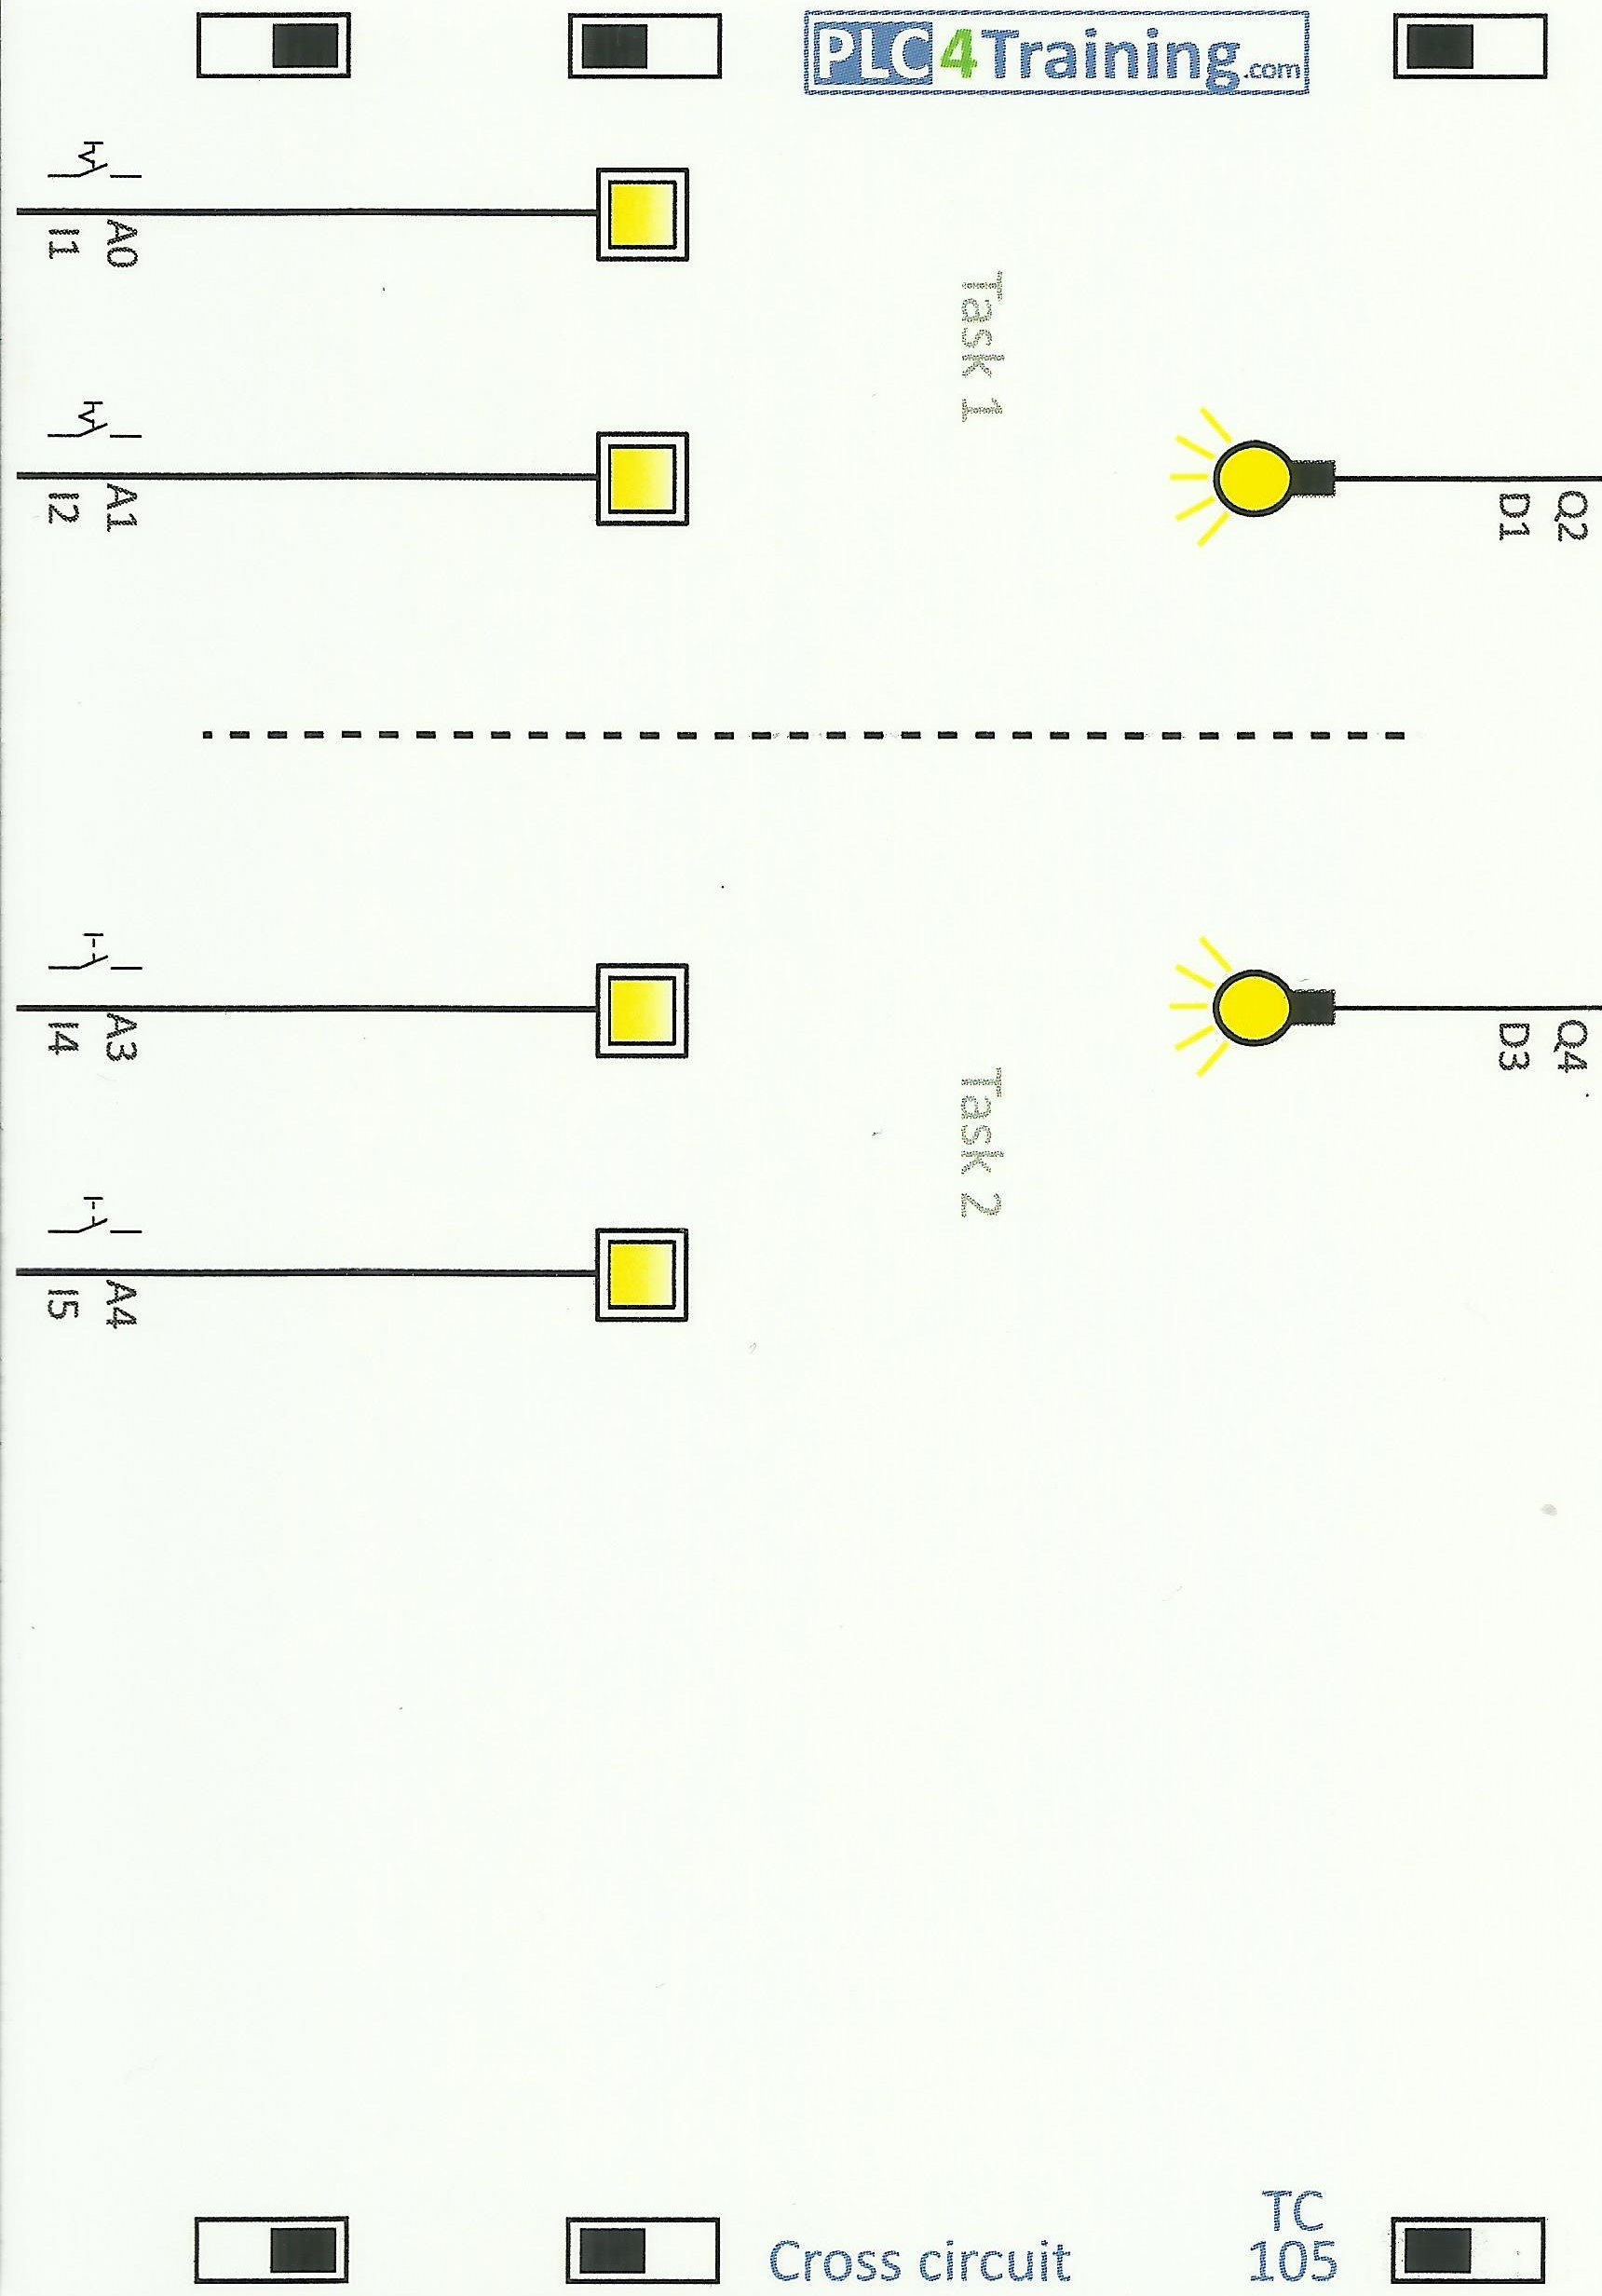
\includegraphics[height=23cm]{105.jpg}}
\captionof{figure}{\texttt{Training Cart 105}}\label{}
\end{center}
\subsubsection{Description du Projet}

Le projet TC 105 a été développé dans le but de présenter deux approches différentes pour la commande d'un éclairage, illustrant un circuit croisé dans la construction électrique conventionnelle. La tâche 1 consiste en une construction électrique conventionnelle avec des interrupteurs, tandis que la tâche 2 propose une implémentation typique avec un automate programmable industriel (PLC) utilisant des boutons comme alternative aux interrupteurs. Chaque tâche vise à offrir une expérience pratique pour les participants.

\subsubsection{Tâches Spécifiques}

\begin{enumerate}
    \item \textbf{Construction Électrique Conventionnelle (Tâche 1):} La première tâche implique la commutation de l'éclairage via deux interrupteurs, reproduisant ainsi un circuit croisé dans la construction électrique conventionnelle. L'utilisation de n'importe quel interrupteur aux entrées \(A_0\) ou \(A_1\) doit permettre d'allumer ou d'éteindre la sortie \(D_1\).
    
    \item \textbf{Implémentation PLC Typique (Tâche 2):} La deuxième tâche propose une solution typique avec un automate programmable industriel (PLC), utilisant des boutons comme alternative aux interrupteurs. L'utilisation de n'importe quel bouton aux entrées \(A_3\) ou \(A_4\) doit permettre d'allumer ou d'éteindre la sortie \(D_3\).
\end{enumerate}

\subsubsection{Capteurs/Actionneurs}

Les composants du projet comprennent des interrupteurs pour les entrées \(A_0\) et \(A_1\) (tâche 1) ainsi que des boutons pour les entrées \(A_3\) et \(A_4\) (tâche 2). Les sorties \(D_1\) et \(D_3\) sont associées à des visualisations d'éclairage, offrant une expérience concrète dans la manipulation de différentes configurations de circuits.

\subsubsection{Code du projet}

\begin{minipage}{0.5\textwidth}
    
\includegraphics[height=3cm]{Code TC105.png}
\end{minipage}%
\begin{minipage}{0.5\textwidth}
    Cliquez sur \href{https://github.com/DexterTaha/Controllino-PLC-Sample/blob/main/TC100/TC105_Circuit_de_croisement/TC105_Circuit_de_croisement.ino}{Code} pour obtenir le code.
\end{minipage}

%TC106\_Connection\_logique--------------------------------------------------------------------------
\newpage
\subsection{TC106\_Connection\_logique}
\begin{center}
\rotatebox[origin=c]{90}{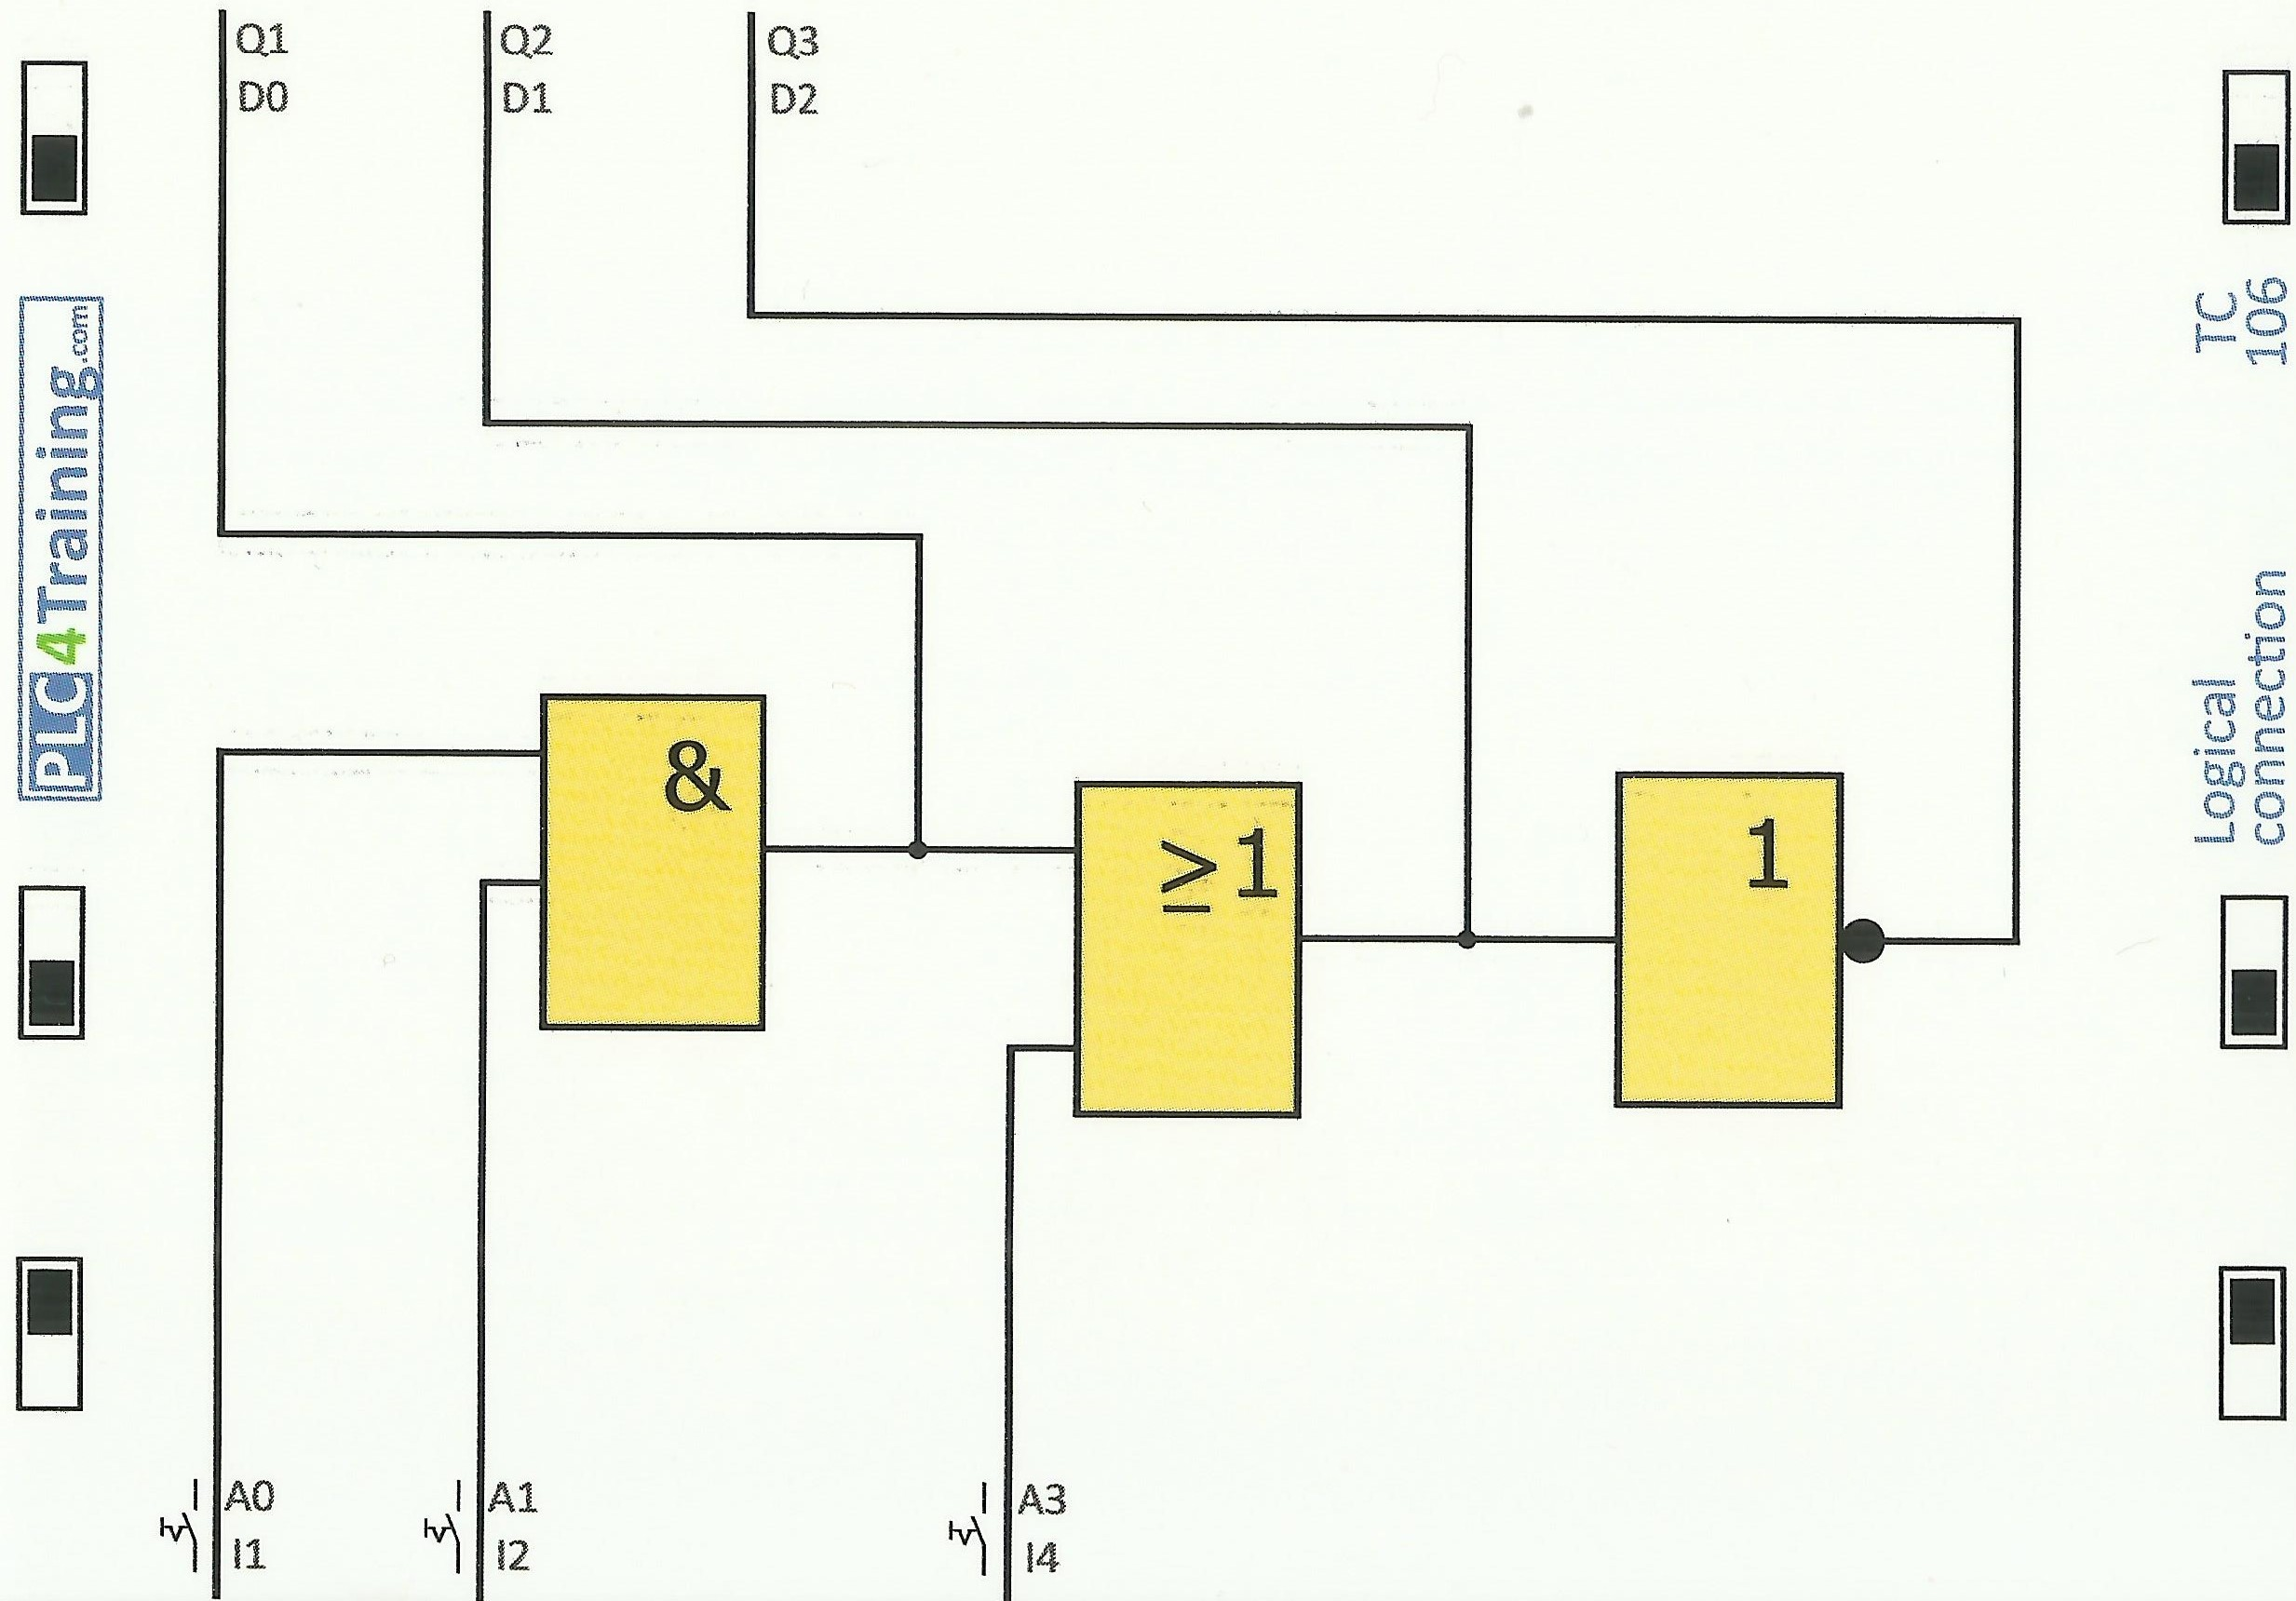
\includegraphics[height=16cm]{106.jpg}}
\captionof{figure}{\texttt{Training Cart 105}}\label{}
\end{center}
\subsubsection{Description du Projet}

Le projet TC 106 a été conçu dans le but de démontrer la création d'une logique complexe à partir de plusieurs blocs logiques distincts. Chaque composant du circuit contribue à la réalisation d'une opération logique globale. La tâche vise à fournir une expérience pratique pour les participants, illustrant la construction d'une logique complexe.

\subsubsection{Tâches Spécifiques}

\begin{enumerate}
    \item \textbf{Connexion Logique (Tâche unique):} La tâche implique que la sortie \(D_0\) ne doit devenir active que si les entrées \(A_0\) et \(A_1\) sont actives simultanément. De plus, la sortie \(D_1\) doit être active si la sortie \(D_0\) ou l'entrée \(A_3\) est active. La sortie \(D_2\) doit représenter une opération NOT de la sortie \(D_1\). Le code \texttt{TC106\_Connection\_logique.ino} fournit une solution complète pour cette tâche.
\end{enumerate}

\subsubsection{Capteurs/Actionneurs}

Les composants du projet comprennent des interrupteurs pour les entrées \(A_0\), \(A_1\) et \(A_3\). Les sorties \(D_0\), \(D_1\) et \(D_2\) sont associées à des LEDs, permettant une visualisation immédiate des résultats des opérations logiques. Cette configuration offre aux participants une expérience concrète dans la manipulation de blocs logiques et la création d'une logique complexe.

\subsubsection{Code du projet}

\begin{minipage}{0.5\textwidth}
    
\includegraphics[height=3cm]{Code TC106.png}
\end{minipage}%
\begin{minipage}{0.5\textwidth}
    Cliquez sur \href{https://github.com/DexterTaha/Controllino-PLC-Sample/blob/main/TC100/TC106_Connection_logique/TC106_Connection_logique.ino}{Code} pour obtenir le code.
\end{minipage}
%TC200--------------------------------------------------------------------------
\newpage
\section{TC200}

Niveau de difficulté 200 :\\

Les tâches et les cartes de formation du niveau 200 sont un peu plus complexes. Une esquisse de tâche peut être programmée dans l'IDE l'IDE Arduino avec quelques lignes de code supplémentaires. Avec un peu de pratique et des connaissances de base, une solution peut être élaborée en 90 minutes. une solution en 90 minutes. Les tâches et les cartes de formation sont numérotées consécutivement : TC 200, TC 201, TC 202 etc.

%TC200\_Alerte\_infirmière--------------------------------------------------------------------------
\newpage
\subsection{TC200\_Alerte\_infirmière}
\begin{center}
\rotatebox[origin=c]{360}{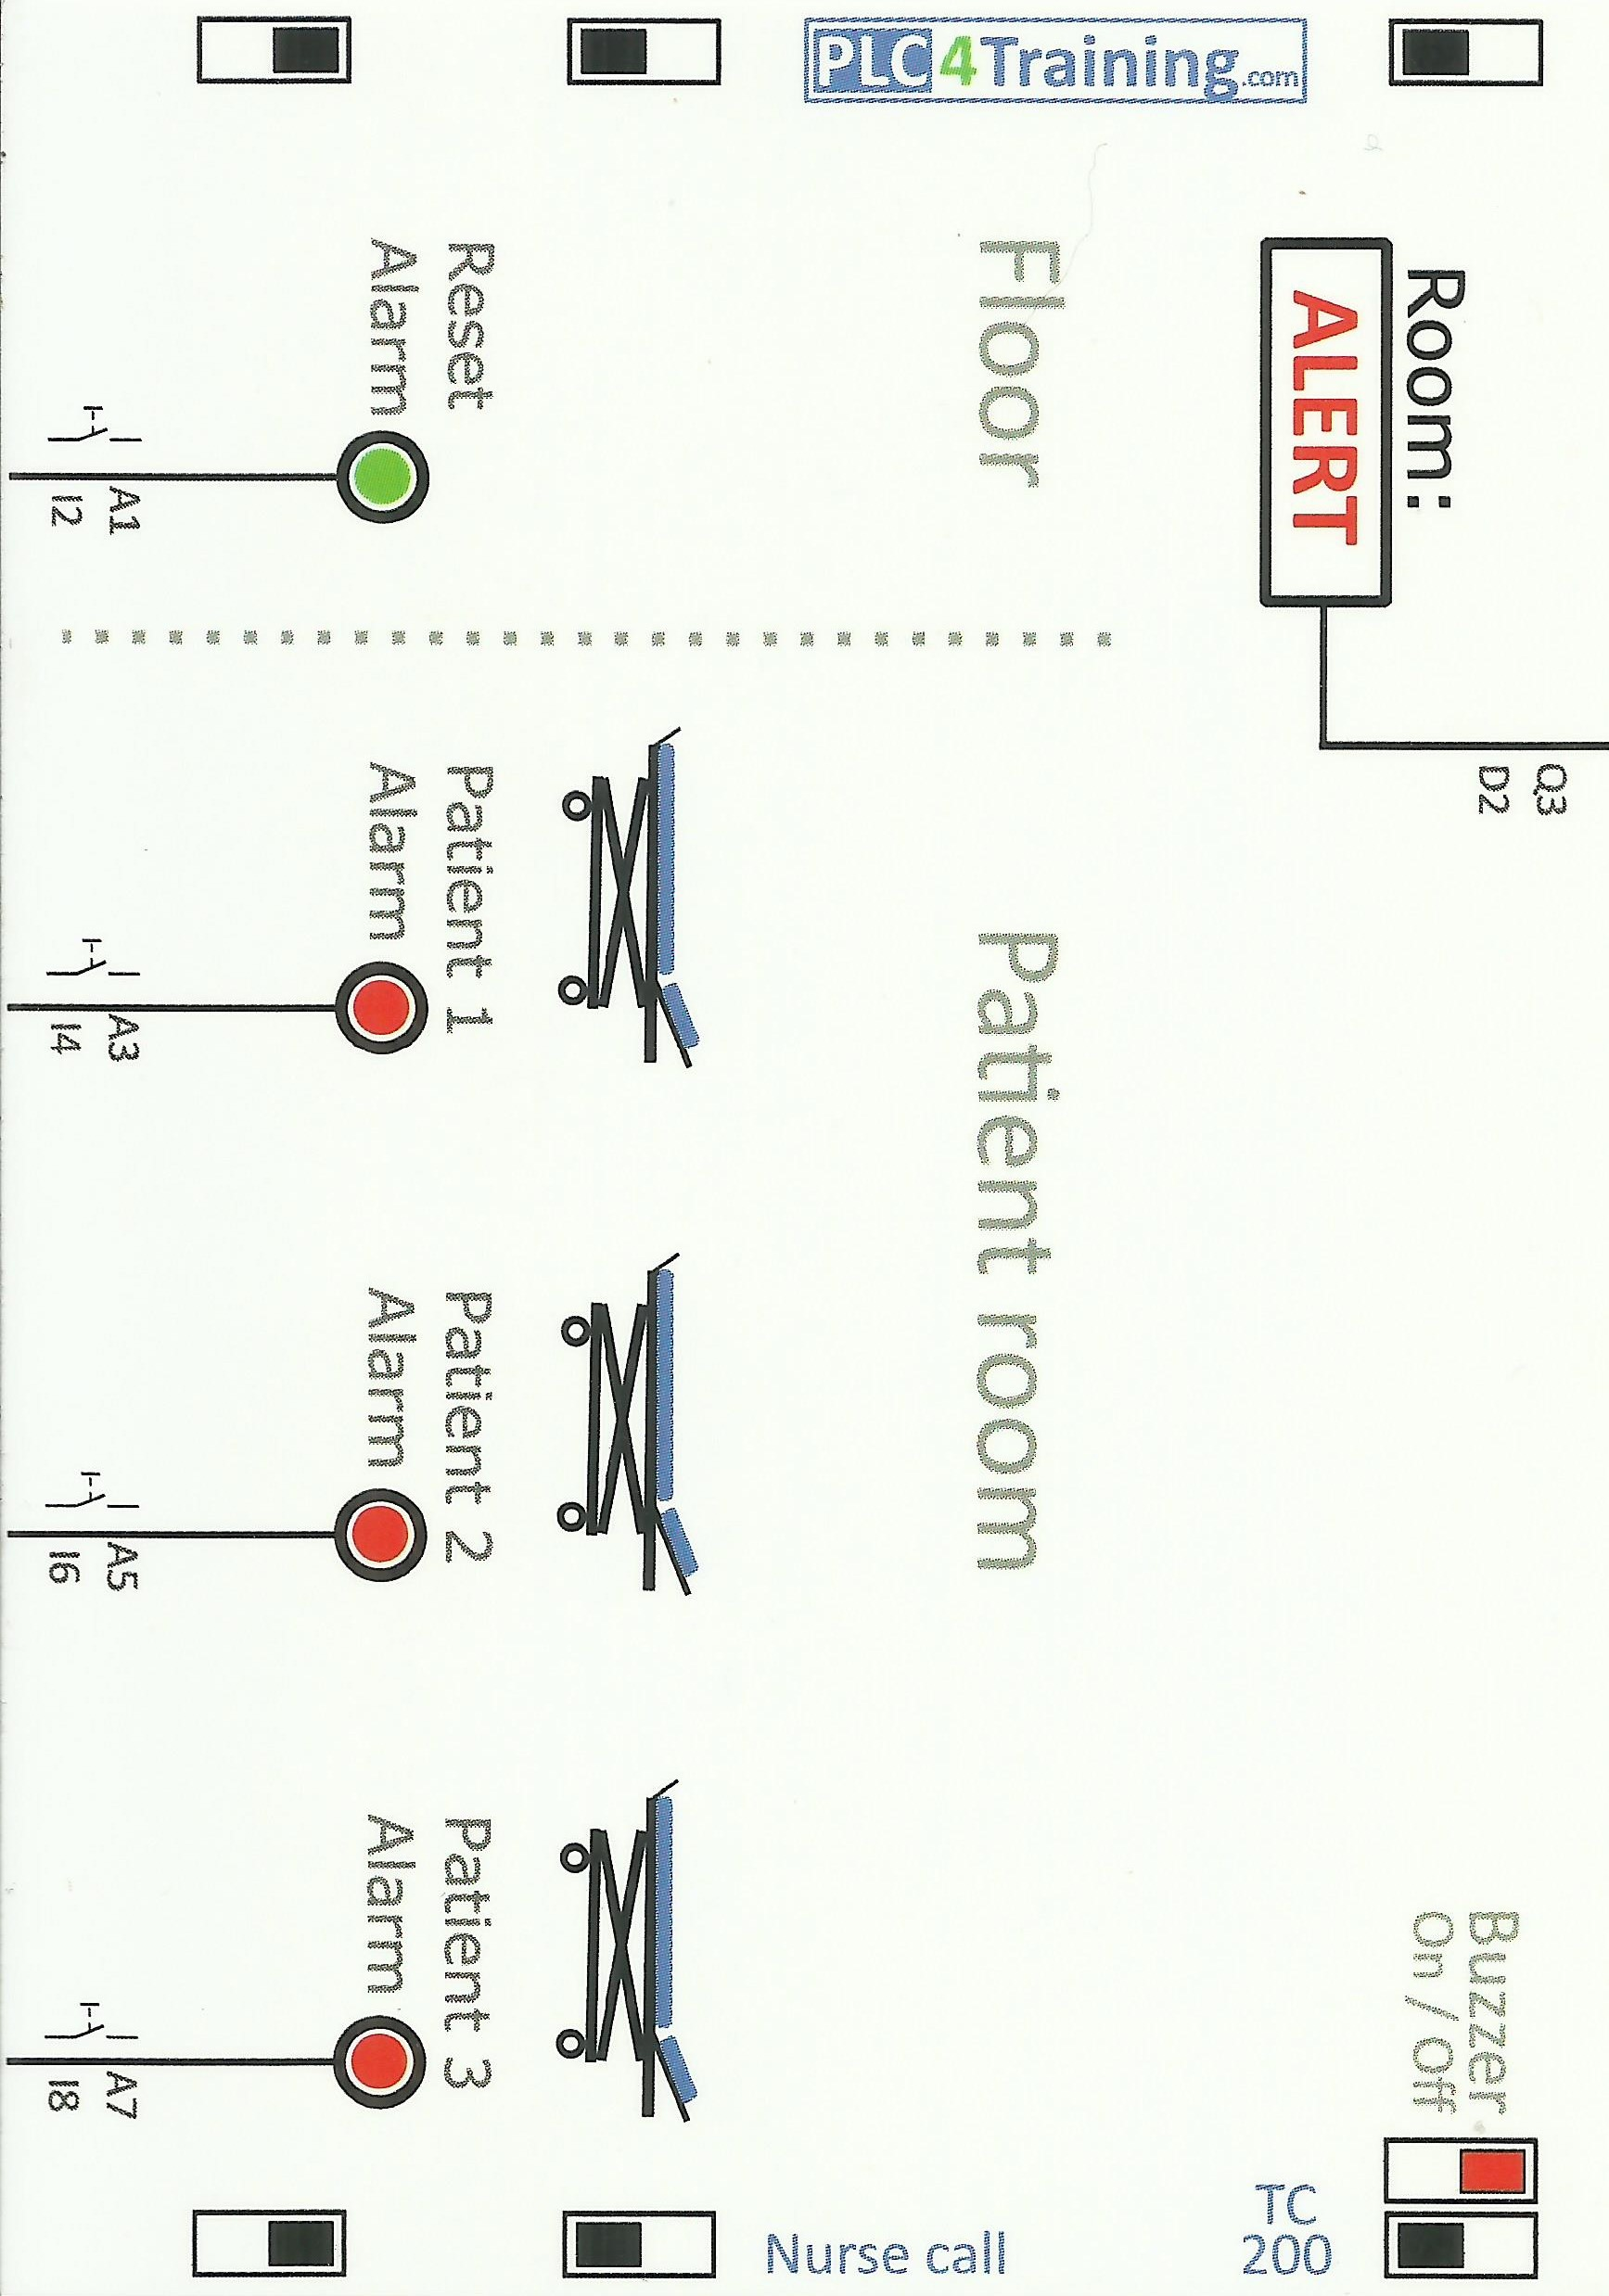
\includegraphics[height=23cm]{200.jpg}}
\captionof{figure}{\texttt{Training Cart 200}}\label{}
\end{center}
\subsubsection{Description du Projet}

Le projet TC 200 a été élaboré dans le but de simuler un système d'appel infirmier pour une chambre de trois lits dans un hôpital. Chaque patient peut déclencher une alarme depuis son lit, et un message d'alarme est émis dans le couloir. La tâche de niveau 200 vise à fournir une expérience pratique de la mise en œuvre d'un système d'appel infirmier.

\subsubsection{Tâches Spécifiques}

\begin{enumerate}
    \item \textbf{Appel Infirmier (Tâche unique):} La tâche consiste à générer une alarme à la sortie \(D_2\) en utilisant trois boutons d'entrée (\(A_3\), \(A_5\), \(A_7\)), chacun associé à un patient spécifique dans la chambre. L'alarme reste active jusqu'à ce qu'elle soit réinitialisée via le bouton \(A_1\) à l'entrée de la chambre. 
\end{enumerate}

\subsubsection{Capteurs/Actionneurs}

Les composants du projet comprennent des boutons pour les entrées \(A_1\), \(A_3\), \(A_5\) et \(A_7\), ainsi que la sortie \(D_2\) qui visualise le message d'alarme. En plus de l'alarme visuelle, un buzzer peut également être activé pour une alarme acoustique. Cette configuration permet aux participants de comprendre la mise en œuvre d'un système d'appel infirmier.

\subsubsection{Code du projet}

\begin{minipage}{0.5\textwidth}
    
\includegraphics[height=3cm]{Code TC200.png}
\end{minipage}%
\begin{minipage}{0.5\textwidth}
    Cliquez sur \href{https://github.com/DexterTaha/Controllino-PLC-Sample/blob/main/TC200/TC200_Alerte_infirmi%C3%A8re/TC200_Alerte_infirmi%C3%A8re.ino}{Code} pour obtenir le code.
\end{minipage}

%TC201\_Lumière\_du\_couloir--------------------------------------------------------------------------
\newpage
\subsection{TC201\_Lumière\_du\_couloir}
\begin{center}
\rotatebox[origin=c]{360}{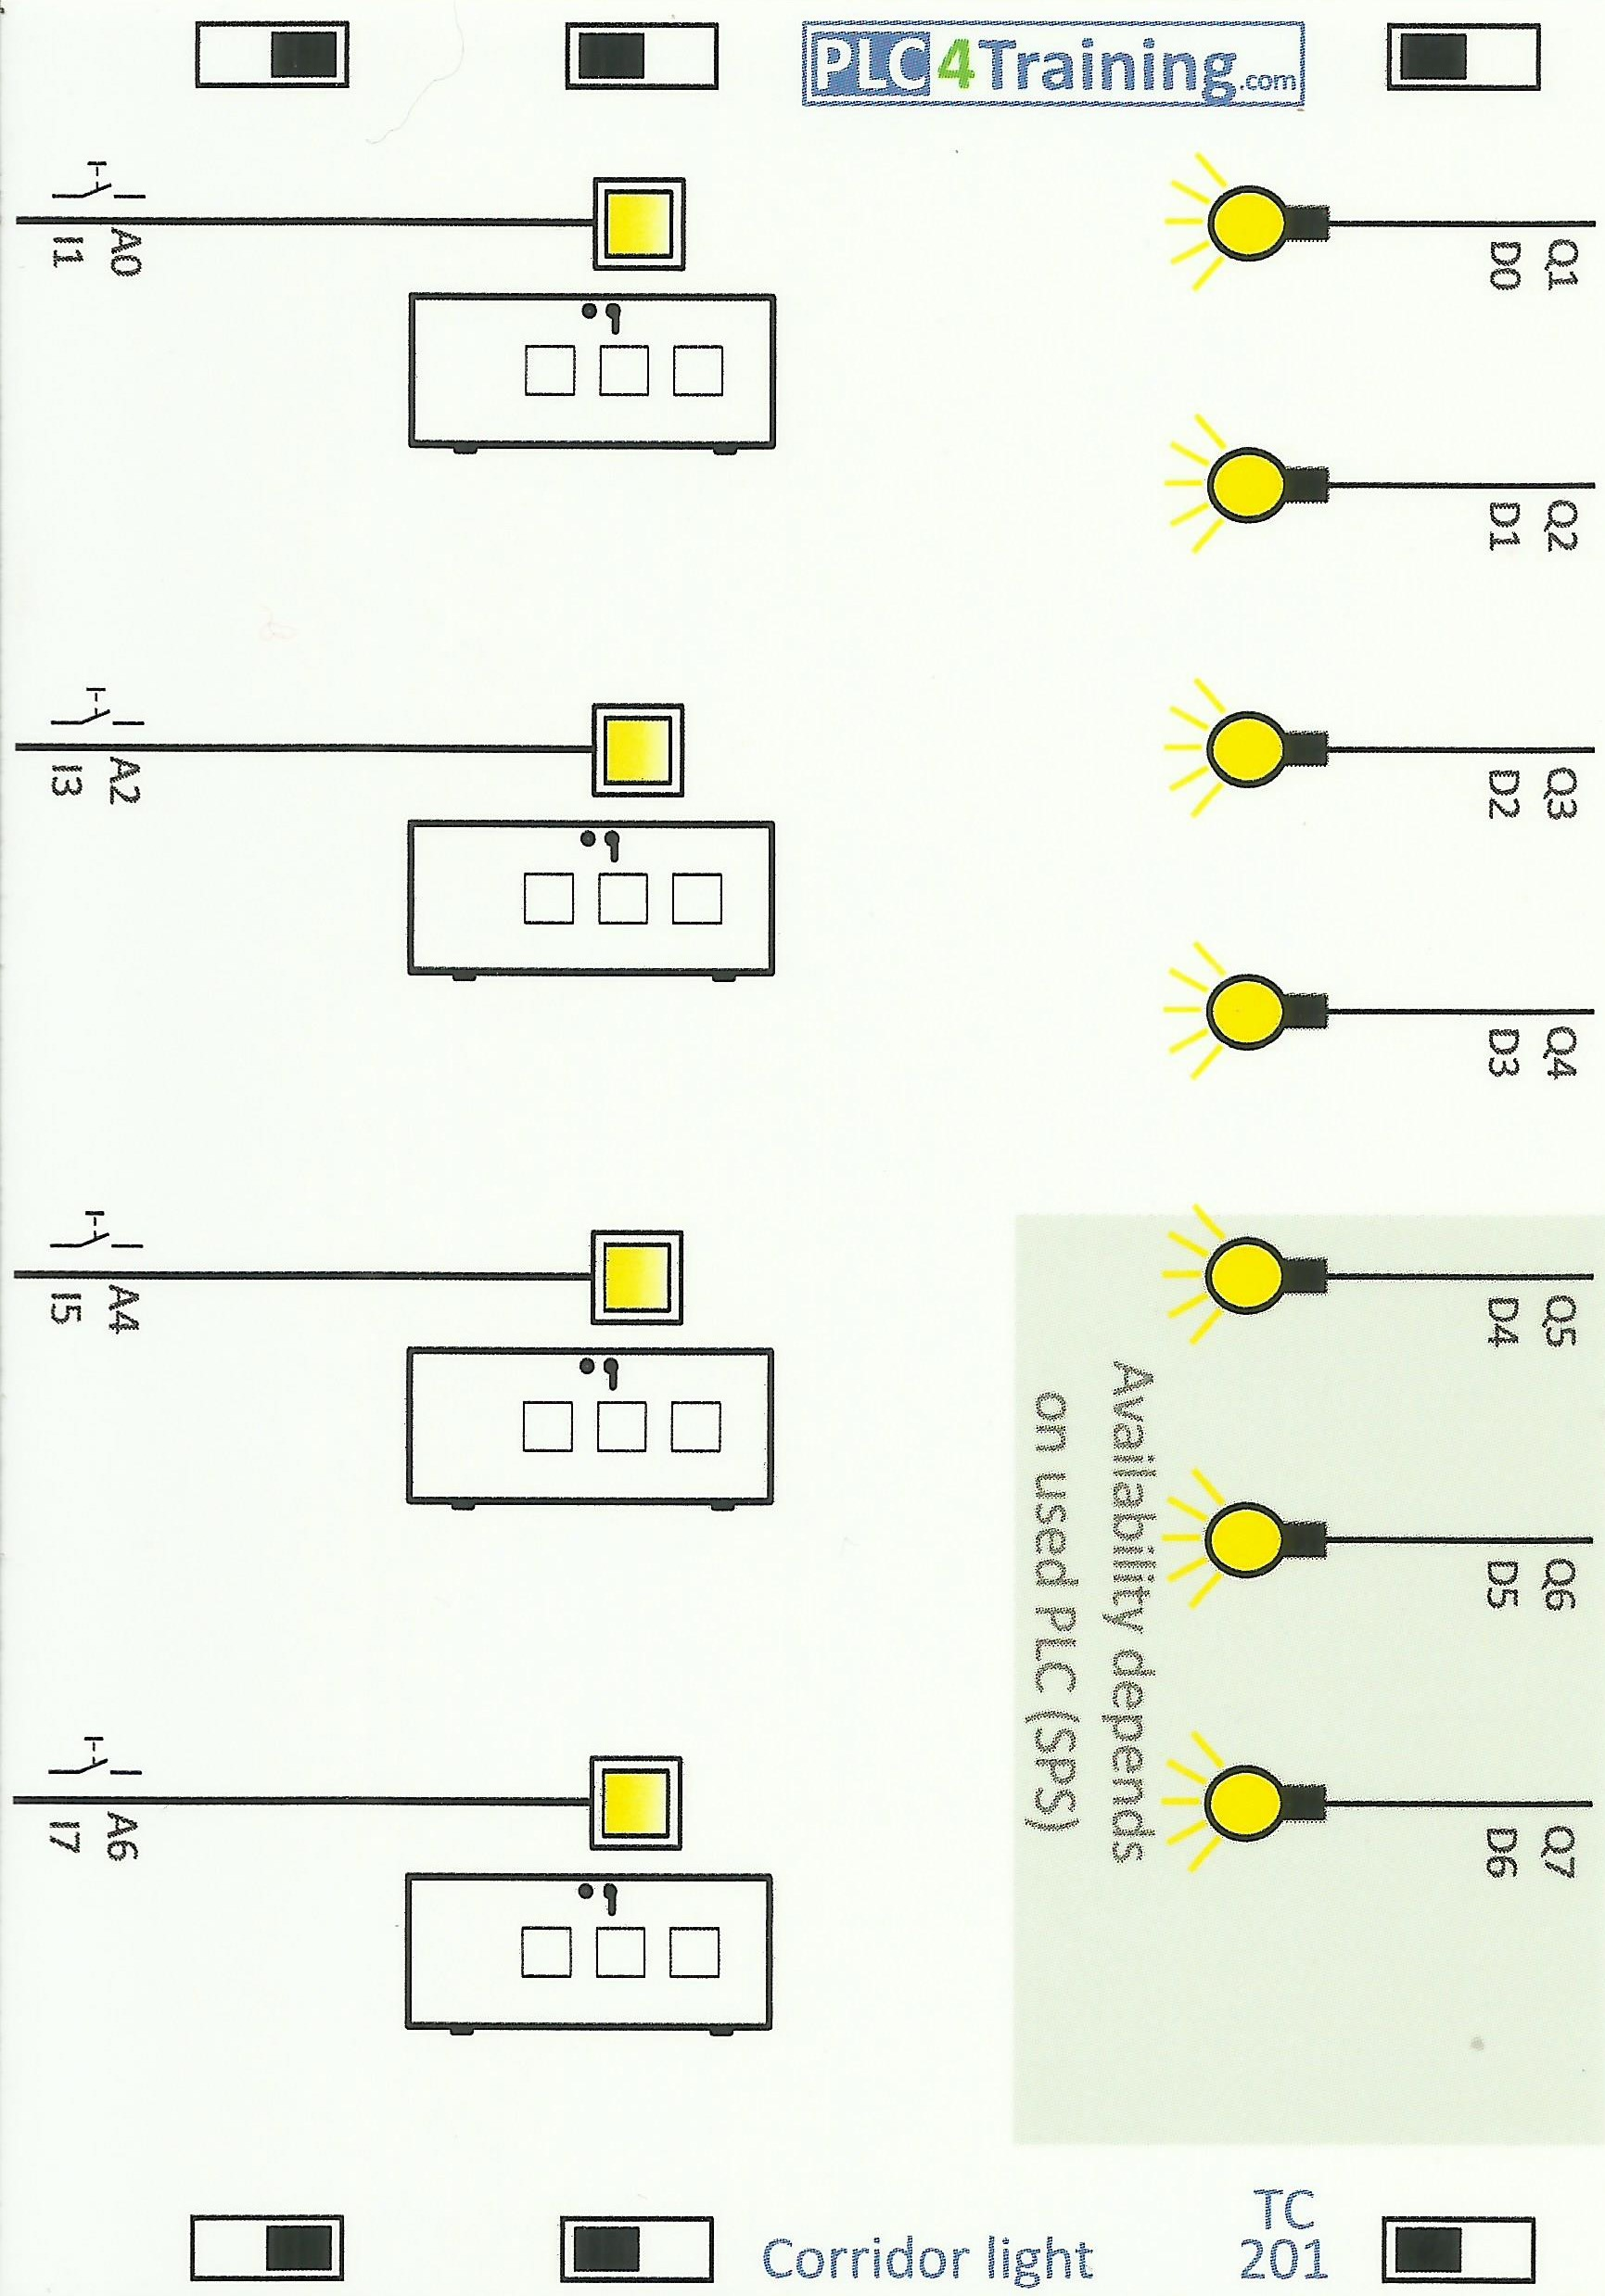
\includegraphics[height=23cm]{201.jpg}}
\captionof{figure}{\texttt{Training Cart 201}}\label{}
\end{center}
\subsubsection{Description du Projet}

Le projet TC 201 a été élaboré dans le but de construire un système de commande d'éclairage pour un long couloir, avec la possibilité d'allumer les lumières à chaque porte d'appartement via un bouton-poussoir. Après un laps de temps spécifié, deux lampes doivent rester allumées brièvement en tant qu'éclairage d'urgence. La tâche de niveau 201 vise à fournir une expérience pratique de la création d'un système de contrôle d'éclairage complexe pour un couloir.

\subsubsection{Tâches Spécifiques}

\begin{enumerate}
    \item \textbf{Contrôle d'Éclairage du Couloir (Tâche unique):} La tâche implique que les boutons aux entrées \(A_0\), \(A_2\), \(A_4\) et \(A_6\) activent l'éclairage du couloir aux sorties \(D_0\) à \(D_3\), simulant ainsi l'éclairage du couloir. Après 10 secondes, seules les sorties \(D_1\) et \(D_5\) doivent être activées pendant 5 secondes en tant qu'éclairage d'urgence. Ensuite, toutes les lampes doivent être éteintes.
\end{enumerate}

\subsubsection{Capteurs/Actionneurs}

Les composants du projet comprennent des boutons pour les entrées \(A_0\), \(A_2\), \(A_4\) et \(A_6\), ainsi que des sorties \(D_0\) à \(D_3\) pour visualiser l'éclairage du couloir. Les sorties \(D_1\) et \(D_5\) sont utilisées pour visualiser l'éclairage d'urgence. Cette configuration permet aux participants de comprendre la mise en œuvre d'un système de contrôle d'éclairage complexe avec des fonctionnalités d'éclairage d'urgence.

\subsubsection{Code du projet}

\begin{minipage}{0.5\textwidth}
    
\includegraphics[height=3cm]{Code TC201.png}
\end{minipage}%
\begin{minipage}{0.5\textwidth}
    Cliquez sur \href{https://github.com/DexterTaha/Controllino-PLC-Sample/blob/main/TC200/TC201_Lumi%C3%A8re_du_couloir/TC201_Lumi%C3%A8re_du_couloir.ino}{Code} pour obtenir le code.
\end{minipage}

%TC202\_Rampe\_élévatrice--------------------------------------------------------------------------
\newpage
\subsection{TC202\_Rampe\_élévatrice}
\begin{center}
\rotatebox[origin=c]{360}{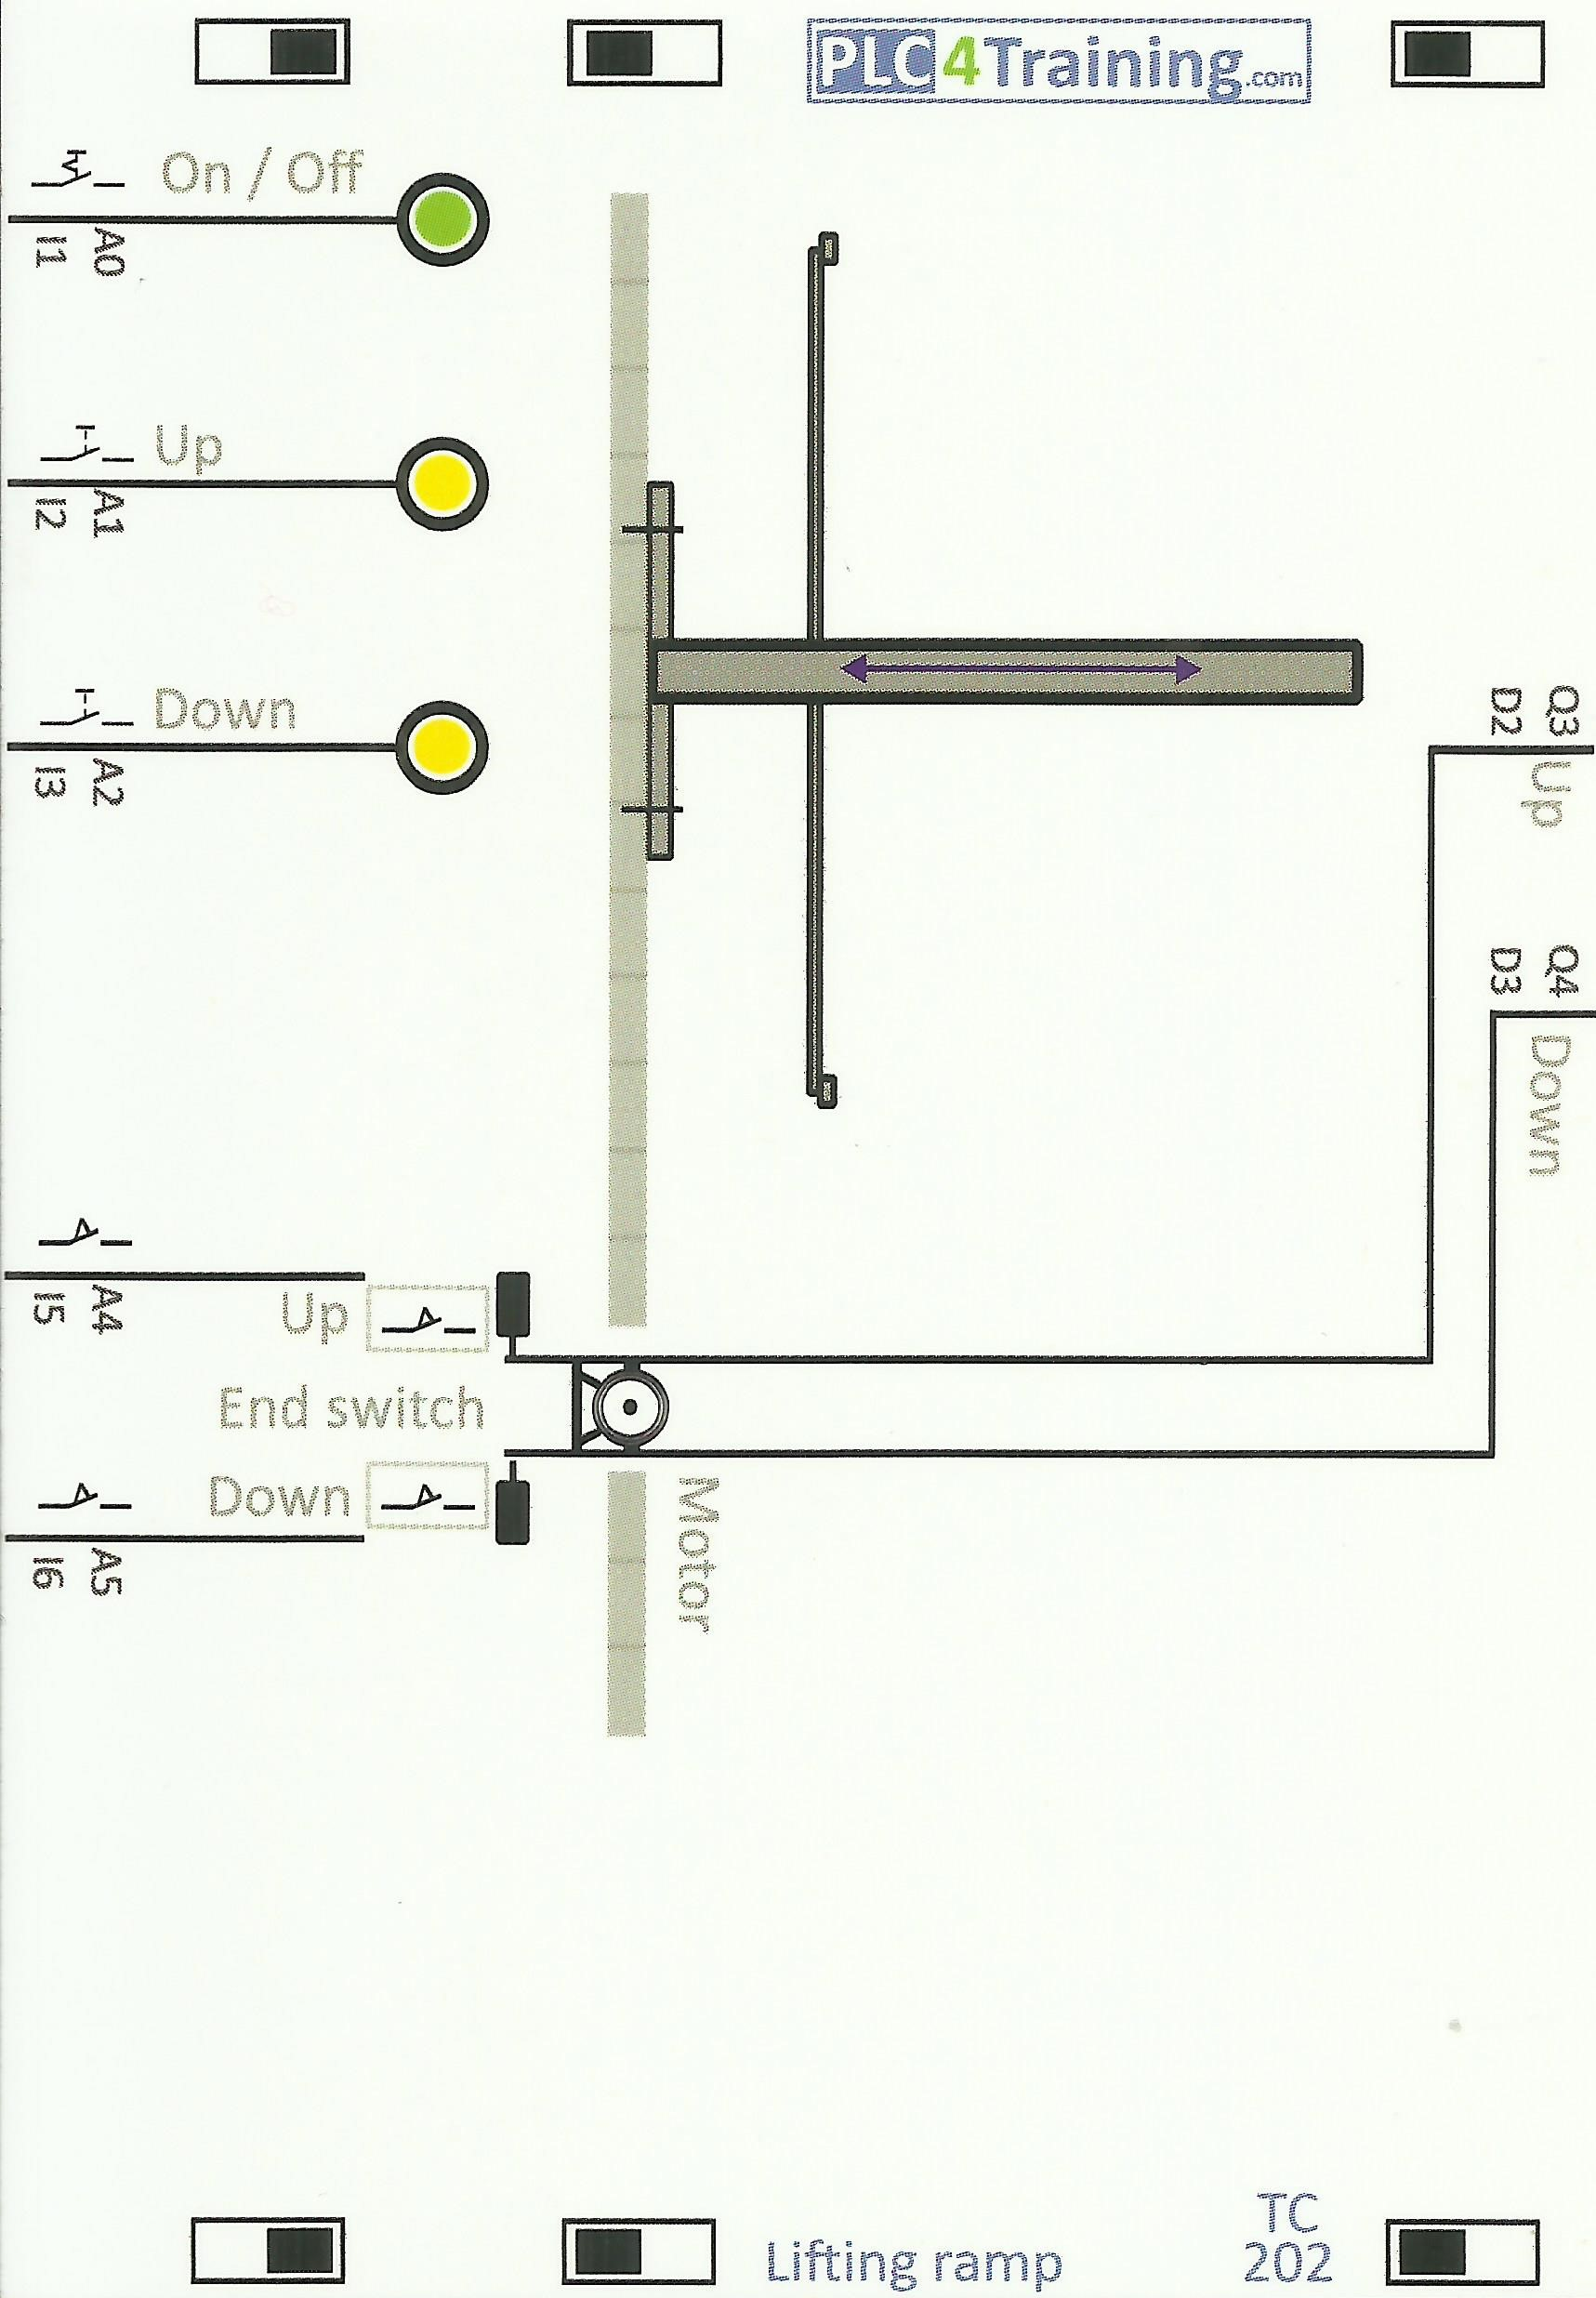
\includegraphics[height=23cm]{202.jpg}}
\captionof{figure}{\texttt{Training Cart 202}}\label{}
\end{center}
\subsubsection{Description du Projet}

Le projet TC 202 a été développé dans le but de simuler la fonction d'une plateforme élévatrice, par exemple, dans un atelier de réparation automobile. La tâche vise à fournir une expérience pratique de la simulation du fonctionnement d'une plateforme élévatrice, avec des fonctionnalités pour allumer/éteindre, monter et descendre la plateforme. Le projet intègre également des interrupteurs de fin de course pour limiter les déplacements de la plateforme.

\subsubsection{Tâches Spécifiques}

\begin{enumerate}
    \item \textbf{Simulation de la Plateforme Élévatrice (Tâche unique):} La tâche consiste à mettre la plateforme élévatrice en service avec l'interrupteur \(A_0\). La plateforme peut être allumée ou éteinte avec cet interrupteur. Lorsque le bouton \(A_1\) est enfoncé, la plateforme monte, et lorsqu'on appuie sur le bouton \(A_2\), elle descend à nouveau. Le moteur est contrôlé avec les sorties \(D_2\) ou \(D_3\), où \(D_2\) signifie "la plateforme monte" et \(D_3\) "la plateforme descend". Les interrupteurs de fin de course \(A_4\) et \(A_5\) limitent les déplacements de la plateforme vers le haut et vers le bas respectivement.
\end{enumerate}

\subsubsection{Capteurs/Actionneurs}

Les composants du projet comprennent des interrupteurs pour les entrées \(A_0\), \(A_1\), \(A_2\), \(A_4\) et \(A_5\), ainsi que des sorties \(D_2\) et \(D_3\) pour visualiser le contrôle du moteur, indiquant si la plateforme monte ou descend. Cette configuration permet aux participants de comprendre la mise en œuvre de la simulation d'une plateforme élévatrice avec des fonctionnalités de contrôle détaillées.

\subsubsection{Code du projet}

\begin{minipage}{0.5\textwidth}
    
\includegraphics[height=3cm]{Code TC202.png}
\end{minipage}%
\begin{minipage}{0.5\textwidth}
    Cliquez sur \href{https://github.com/DexterTaha/Controllino-PLC-Sample/blob/main/TC200/TC202_Rampe_%C3%A9l%C3%A9vatrice/TC202_Rampe_%C3%A9l%C3%A9vatrice.ino}{Code} pour obtenir le code.
\end{minipage}

%TC203\_Sens\_de\_rotation--------------------------------------------------------------------------
\newpage
\subsection{TC203\_Sens\_de\_rotation}
\begin{center}
\rotatebox[origin=c]{360}{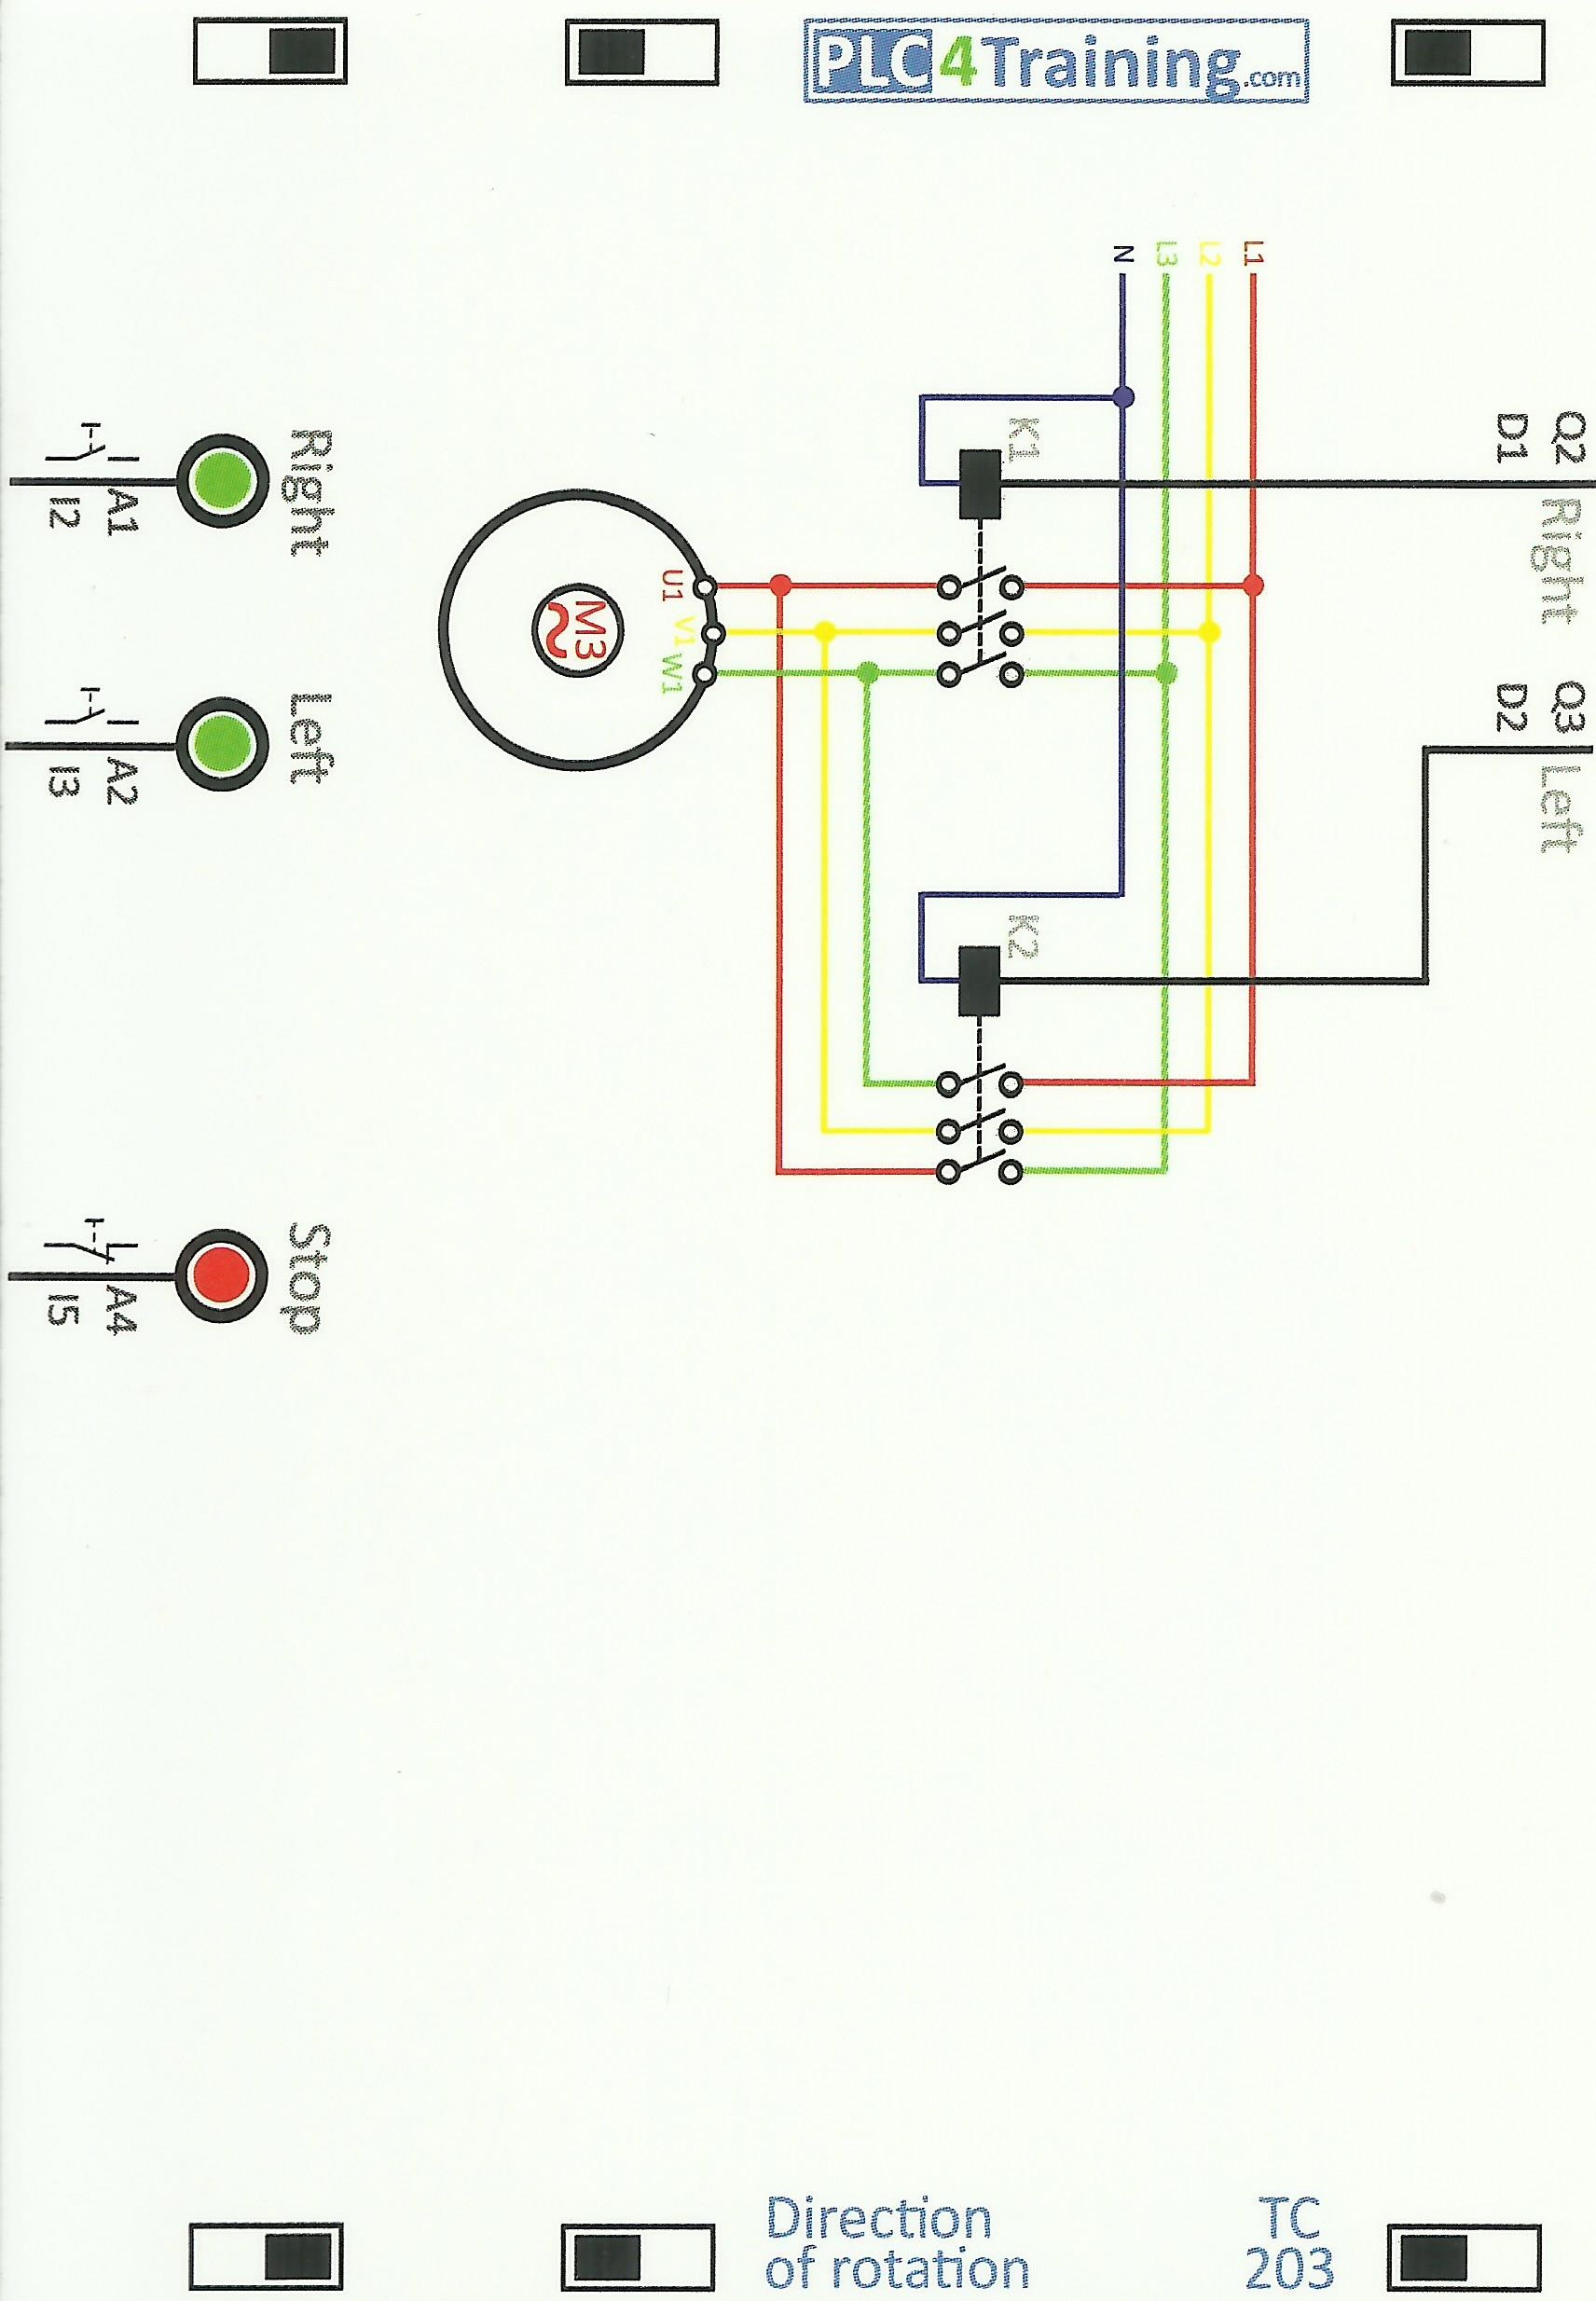
\includegraphics[height=23cm]{203.jpg}}
\captionof{figure}{\texttt{Training Cart 203}}\label{}
\end{center}
\subsubsection{Description du Projet}

Le projet TC 203 a été développé dans le but de simuler le fonctionnement d'un moteur triphasé en rotation horaire ou antihoraire. La tâche vise à fournir une expérience pratique de la mise en œuvre du contrôle de la direction de rotation d'un moteur, avec des fonctionnalités pour démarrer, arrêter et changer la direction de rotation après une pause spécifiée.

\subsubsection{Tâches Spécifiques}

\begin{enumerate}
    \item \textbf{Commande de la Direction de Rotation (Tâche unique):} La tâche implique que le moteur soit démarré en direction horaire avec le bouton \(A_1\) et en direction antihoraire avec le bouton \(A_2\). Le moteur peut être arrêté avec le bouton \(A_4\) (contact normalement fermé). La direction de rotation ne peut être modifiée qu'après l'arrêt du moteur via le bouton-poussoir \(A_4\) et après une pause de 5 secondes. Cela garantit que le moteur ne peut pas être commuté directement d'une direction de rotation à l'autre.
\end{enumerate}

\subsubsection{Capteurs/Actionneurs}

Les composants du projet comprennent des boutons pour les entrées \(A_1\), \(A_2\) et \(A_4\), ainsi que des sorties \(D_1\) et \(D_2\) pour visualiser la direction de rotation dans les sens horaire et antihoraire. Cette configuration permet aux participants de comprendre la mise en œuvre du contrôle de la direction de rotation d'un moteur triphasé, y compris les fonctionnalités de démarrage, d'arrêt et de changement de direction.

\subsubsection{Code du projet}

\begin{minipage}{0.5\textwidth}
    
\includegraphics[height=3cm]{Code TC203.png}
\end{minipage}%
\begin{minipage}{0.5\textwidth}
    Cliquez sur \href{https://github.com/DexterTaha/Controllino-PLC-Sample/blob/main/TC200/TC203_Sens_de_rotation/TC203_Sens_de_rotation.ino}{Code} pour obtenir le code.
\end{minipage}

%TC204\_Circuit\_étoile\_triangle--------------------------------------------------------------------------
\newpage
\subsection{TC204\_Circuit\_étoile\_triangle}
\begin{center}
\rotatebox[origin=c]{360}{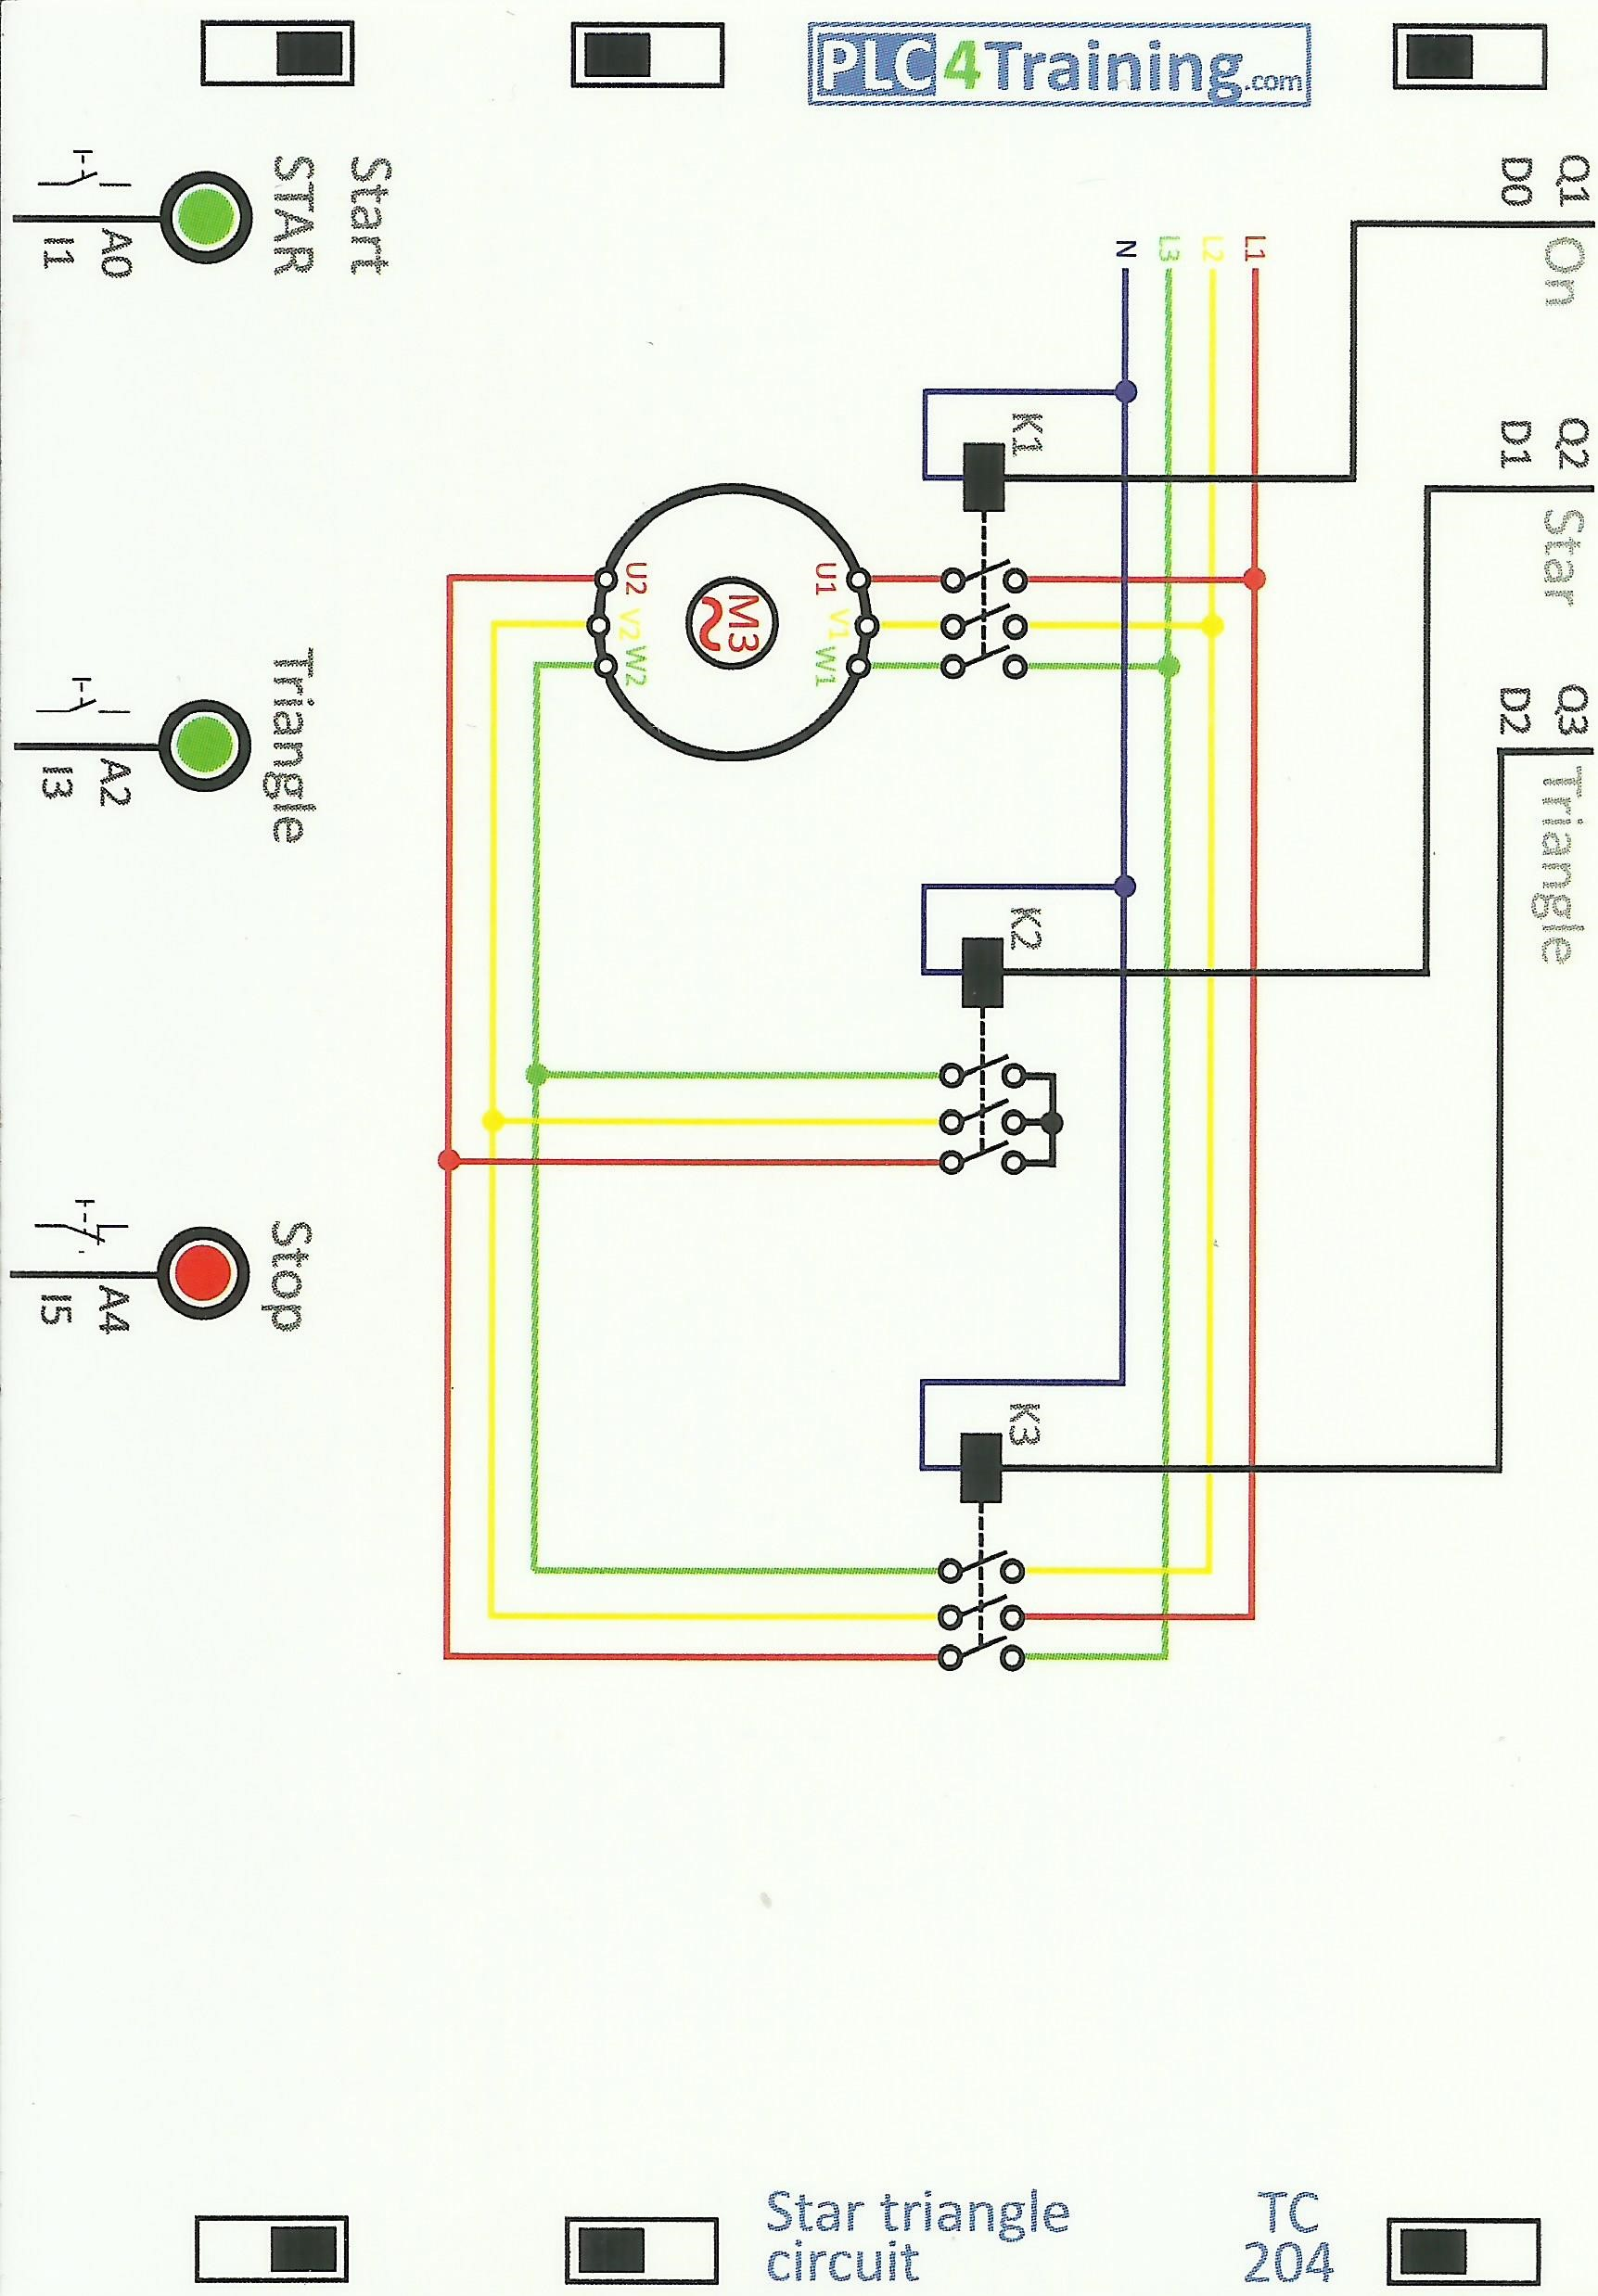
\includegraphics[height=23cm]{204.jpg}}
\captionof{figure}{\texttt{Training Cart 204}}\label{}
\end{center}
\subsubsection{Description du Projet}

Le projet TC 204 a été conçu pour simuler le fonctionnement d'un moteur triphasé dans un circuit étoile-triangle. La tâche vise à fournir une expérience pratique de la mise en œuvre du contrôle de démarrage et d'arrêt d'un moteur triphasé, ainsi que du basculement entre les modes étoile et triangle après une période spécifiée.

\subsubsection{Tâches Spécifiques}

\begin{enumerate}
    \item \textbf{Circuit Étoile-Triangle (Tâche 1):} 
    La première tâche implique de démarrer le moteur triphasé en circuit étoile en appuyant sur le bouton \(A_0\). Cela se fait en contrôlant simultanément les sorties \(D_0\) et \(D_1\). Au plus tôt 3 secondes après, le moteur peut être basculé en mode triangle en appuyant sur le bouton \(A_2\). Pour ce faire, la sortie \(D_1\) doit d'abord être éteinte, et la sortie \(D_2\) doit être allumée seulement après. Le moteur peut être arrêté à tout moment en appuyant sur le bouton \(A_4\), éteignant toutes les sorties.
    
    \item \textbf{Circuit Étoile-Triangle avec Démarrage Automatique (Tâche 2):} 
    La deuxième tâche consiste à démarrer le moteur triphasé en mode étoile en appuyant sur le bouton \(A_0\). Cela se fait en contrôlant simultanément les sorties \(D_0\) et \(D_1\). Après 10 secondes, le moteur doit basculer automatiquement en mode triangle. Pour ce faire, la sortie \(D_1\) doit d'abord être éteinte, et la sortie \(D_2\) doit être allumée seulement après. Le moteur peut être arrêté à tout moment en appuyant sur le bouton \(A_4\), éteignant toutes les sorties.
\end{enumerate}
\subsubsection{Capteurs/Actionneurs}

Les composants du projet comprennent des boutons pour les entrées \(A_0\), \(A_2\) et \(A_4\), ainsi que des sorties \(D_0\), \(D_1\) et \(D_2\) pour visualiser le contrôle des contacteurs principaux, du contacteur étoile et du contacteur triangle. Cette configuration permet aux participants de comprendre la mise en œuvre du contrôle du moteur triphasé dans un circuit étoile-triangle.

\subsubsection{Code du projet}

\begin{minipage}{0.5\textwidth}
    
\includegraphics[height=3cm]{Code TC204.png}
\end{minipage}%
\begin{minipage}{0.5\textwidth}
    Cliquez sur \href{https://github.com/DexterTaha/Controllino-PLC-Sample/blob/main/TC200/TC204_Circuit_%C3%A9toile_triangle/TC204_Circuit_%C3%A9toile_triangle.ino}{Code} pour obtenir le code.
\end{minipage}

%TC205\_Surveillance\_de\_niveau--------------------------------------------------------------------------
\newpage
\subsection{TC205\_Surveillance\_de\_niveau}
\begin{center}
\rotatebox[origin=c]{360}{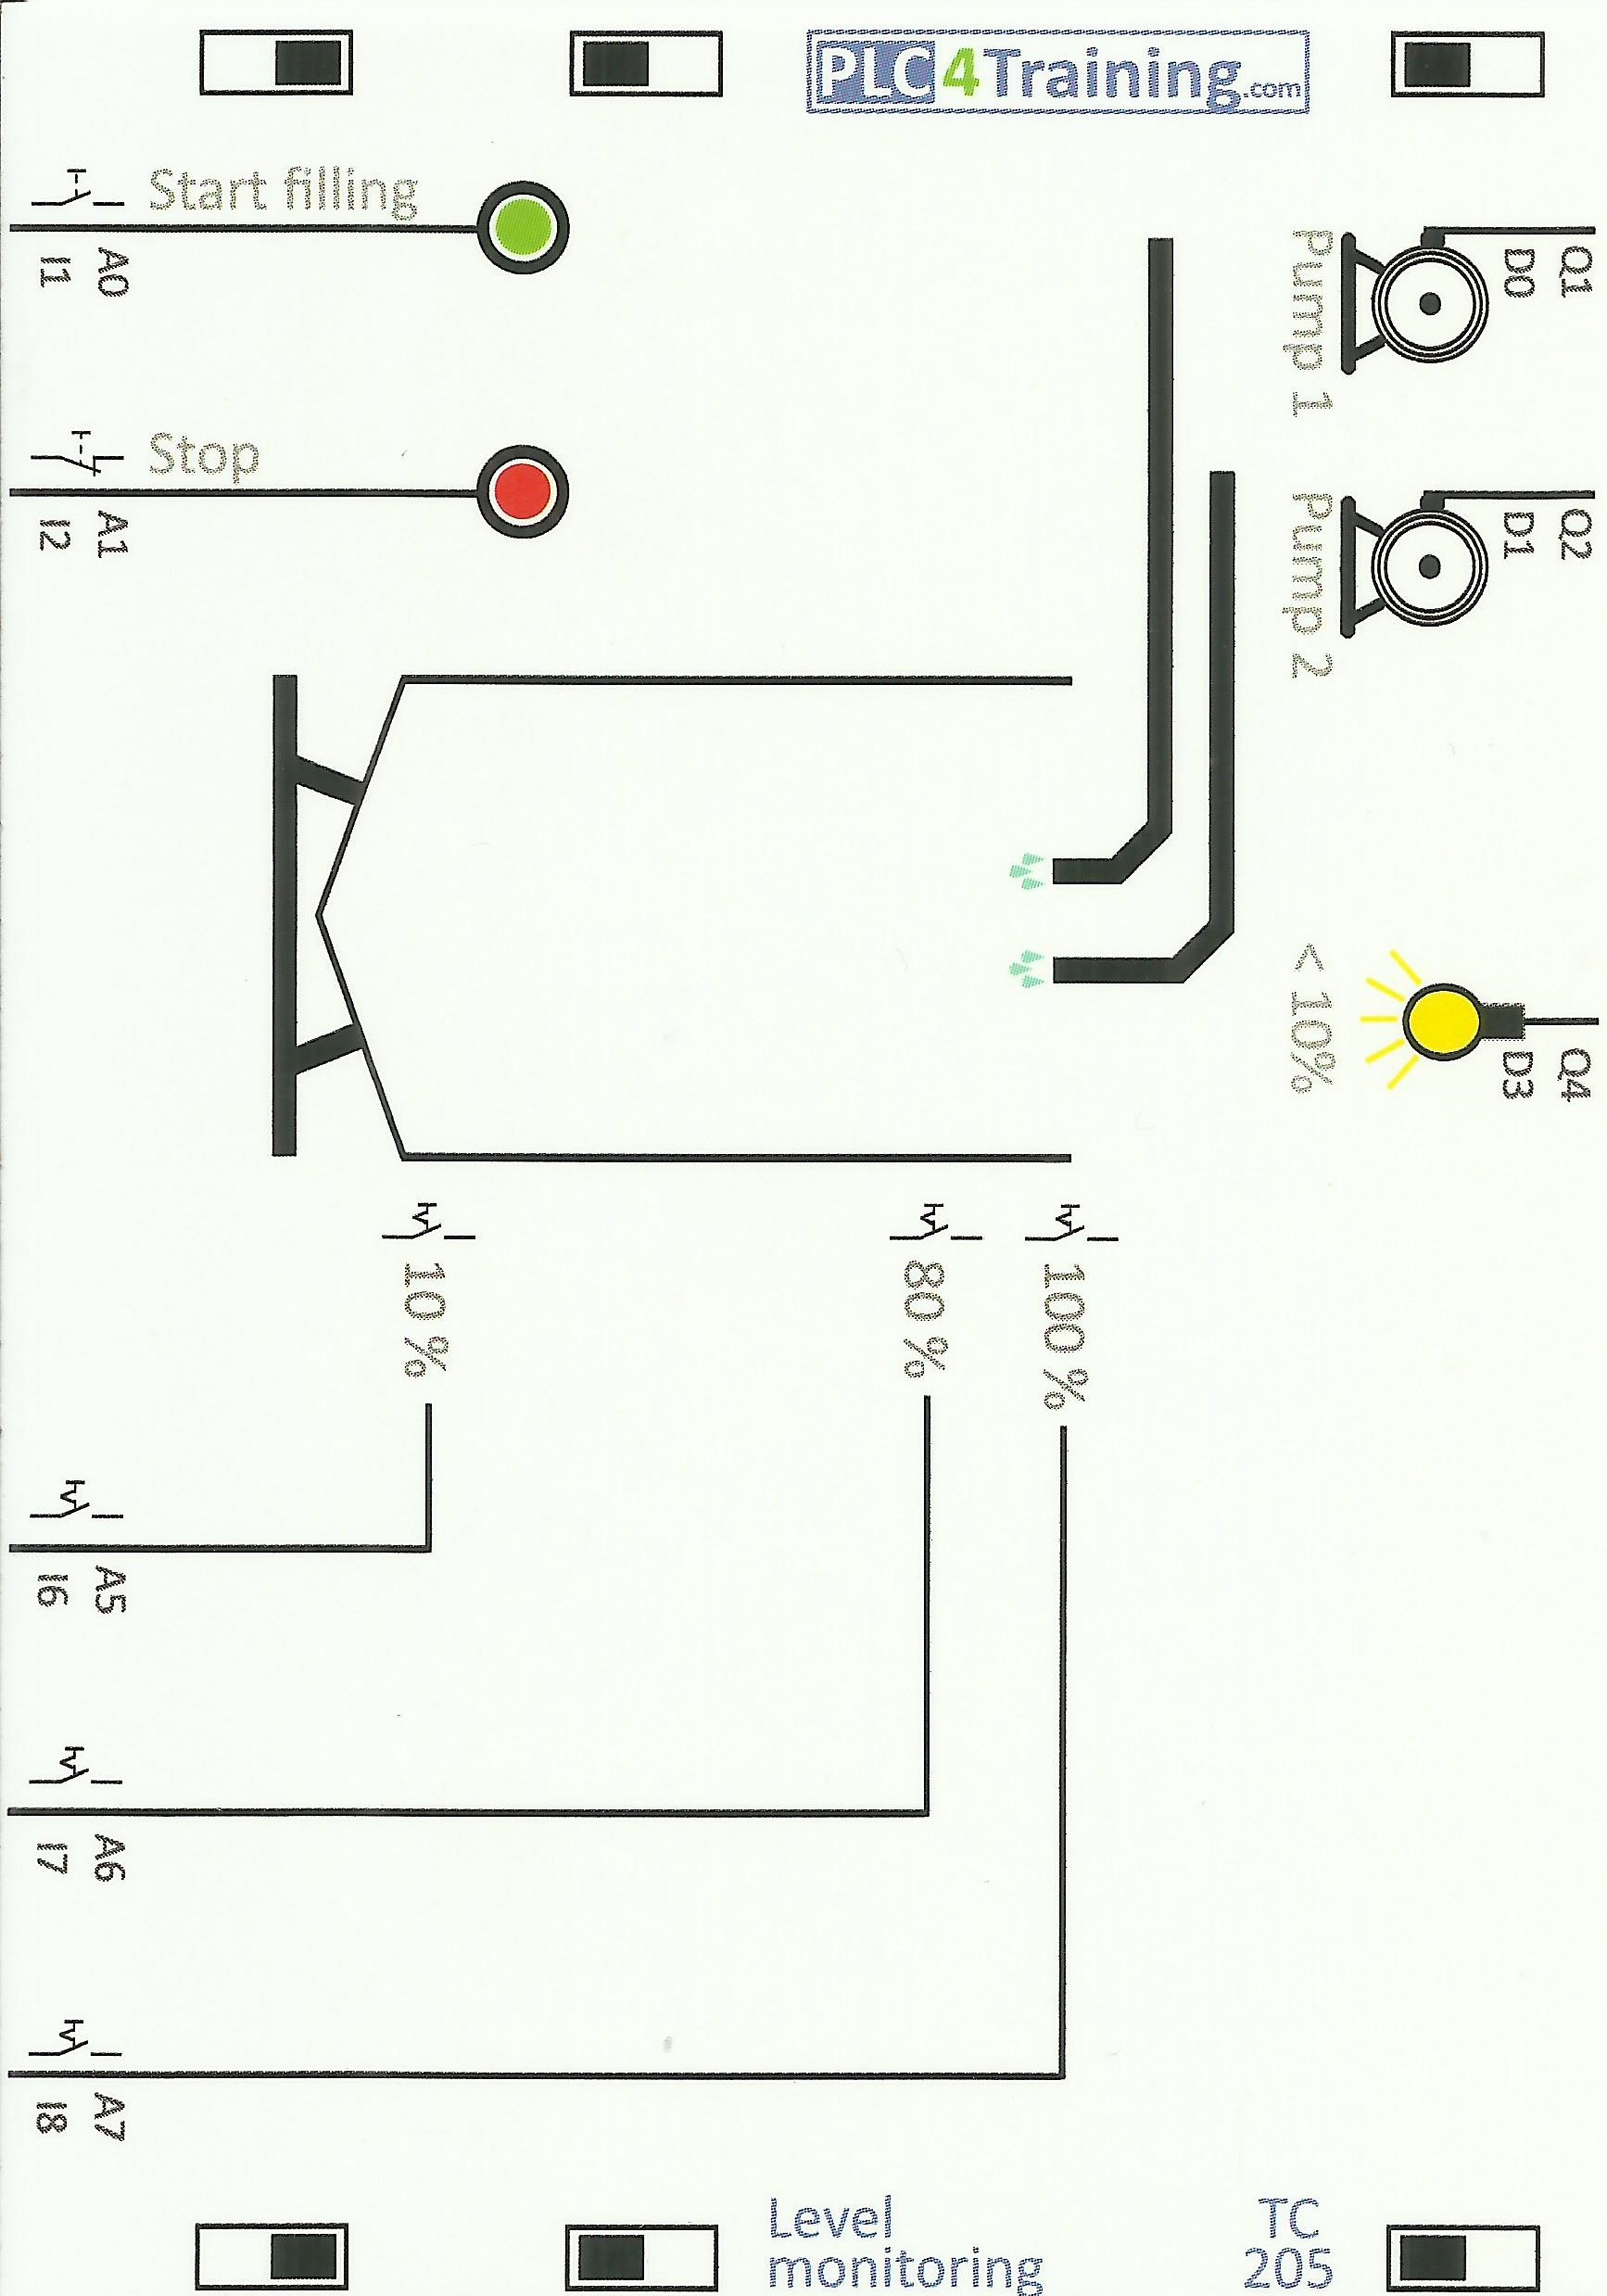
\includegraphics[height=23cm]{205.jpg}}
\captionof{figure}{\texttt{Training Cart 205}}\label{}
\end{center}
\subsubsection{Description du Projet}

Le projet TC 205 a été développé dans le but de simuler le remplissage d'un réservoir à l'aide de deux pompes et d'un interrupteur à flotteur servant de protection contre le débordement. La tâche vise à fournir une expérience pratique de la mise en œuvre du contrôle du niveau de remplissage d'un réservoir, intégrant des fonctionnalités telles que le démarrage et l'arrêt du remplissage, la gestion de deux pompes, et la détection de niveaux critiques.

\subsubsection{Tâches Spécifiques}

\begin{enumerate}
    \item \textbf{Surveillance du Niveau (Tâche unique):} La tâche implique de démarrer le remplissage du réservoir avec le bouton \(A_0\), pouvant être arrêté à tout moment avec le bouton \(A_1\) (contact normalement fermé). Le remplissage est effectué jusqu'à 80\% (capteur \(A_6\)) avec deux pompes (sorties \(D_0\) et \(D_1\)), puis jusqu'à 100\% (capteur \(A_7\)) avec une seule pompe (sortie \(D_0\)). Si le niveau dans le réservoir tombe en dessous de 10\% (capteur \(A_5\)), cela est signalé à la sortie \(D_3\). Un nouveau remplissage du réservoir doit être démarré avec le bouton \(A_0\).
\end{enumerate}

\subsubsection{Capteurs/Actionneurs}

Les composants du projet comprennent des boutons pour les entrées \(A_0\), \(A_1\), \(A_5\), \(A_6\) et \(A_7\), ainsi que des sorties \(D_0\), \(D_1\) et \(D_3\) pour visualiser le fonctionnement des pompes et l'indicateur de niveau. Cette configuration permet aux participants de comprendre la mise en œuvre du contrôle du niveau de remplissage d'un réservoir avec des fonctionnalités détaillées.

\subsubsection{Code du projet}

\begin{minipage}{0.5\textwidth}
    
\includegraphics[height=3cm]{Code TC205.png}
\end{minipage}%
\begin{minipage}{0.5\textwidth}
    Cliquez sur \href{https://github.com/DexterTaha/Controllino-PLC-Sample/blob/main/TC200/TC205_Surveillance_de_niveau/TC205_Surveillance_de_niveau.ino}{Code} pour obtenir le code.
\end{minipage}

%TC206\_Surveillance\_de\_niveau\_2--------------------------------------------------------------------------
\newpage
\subsection{TC206\_Surveillance\_de\_niveau\_2}
\begin{center}
\rotatebox[origin=c]{360}{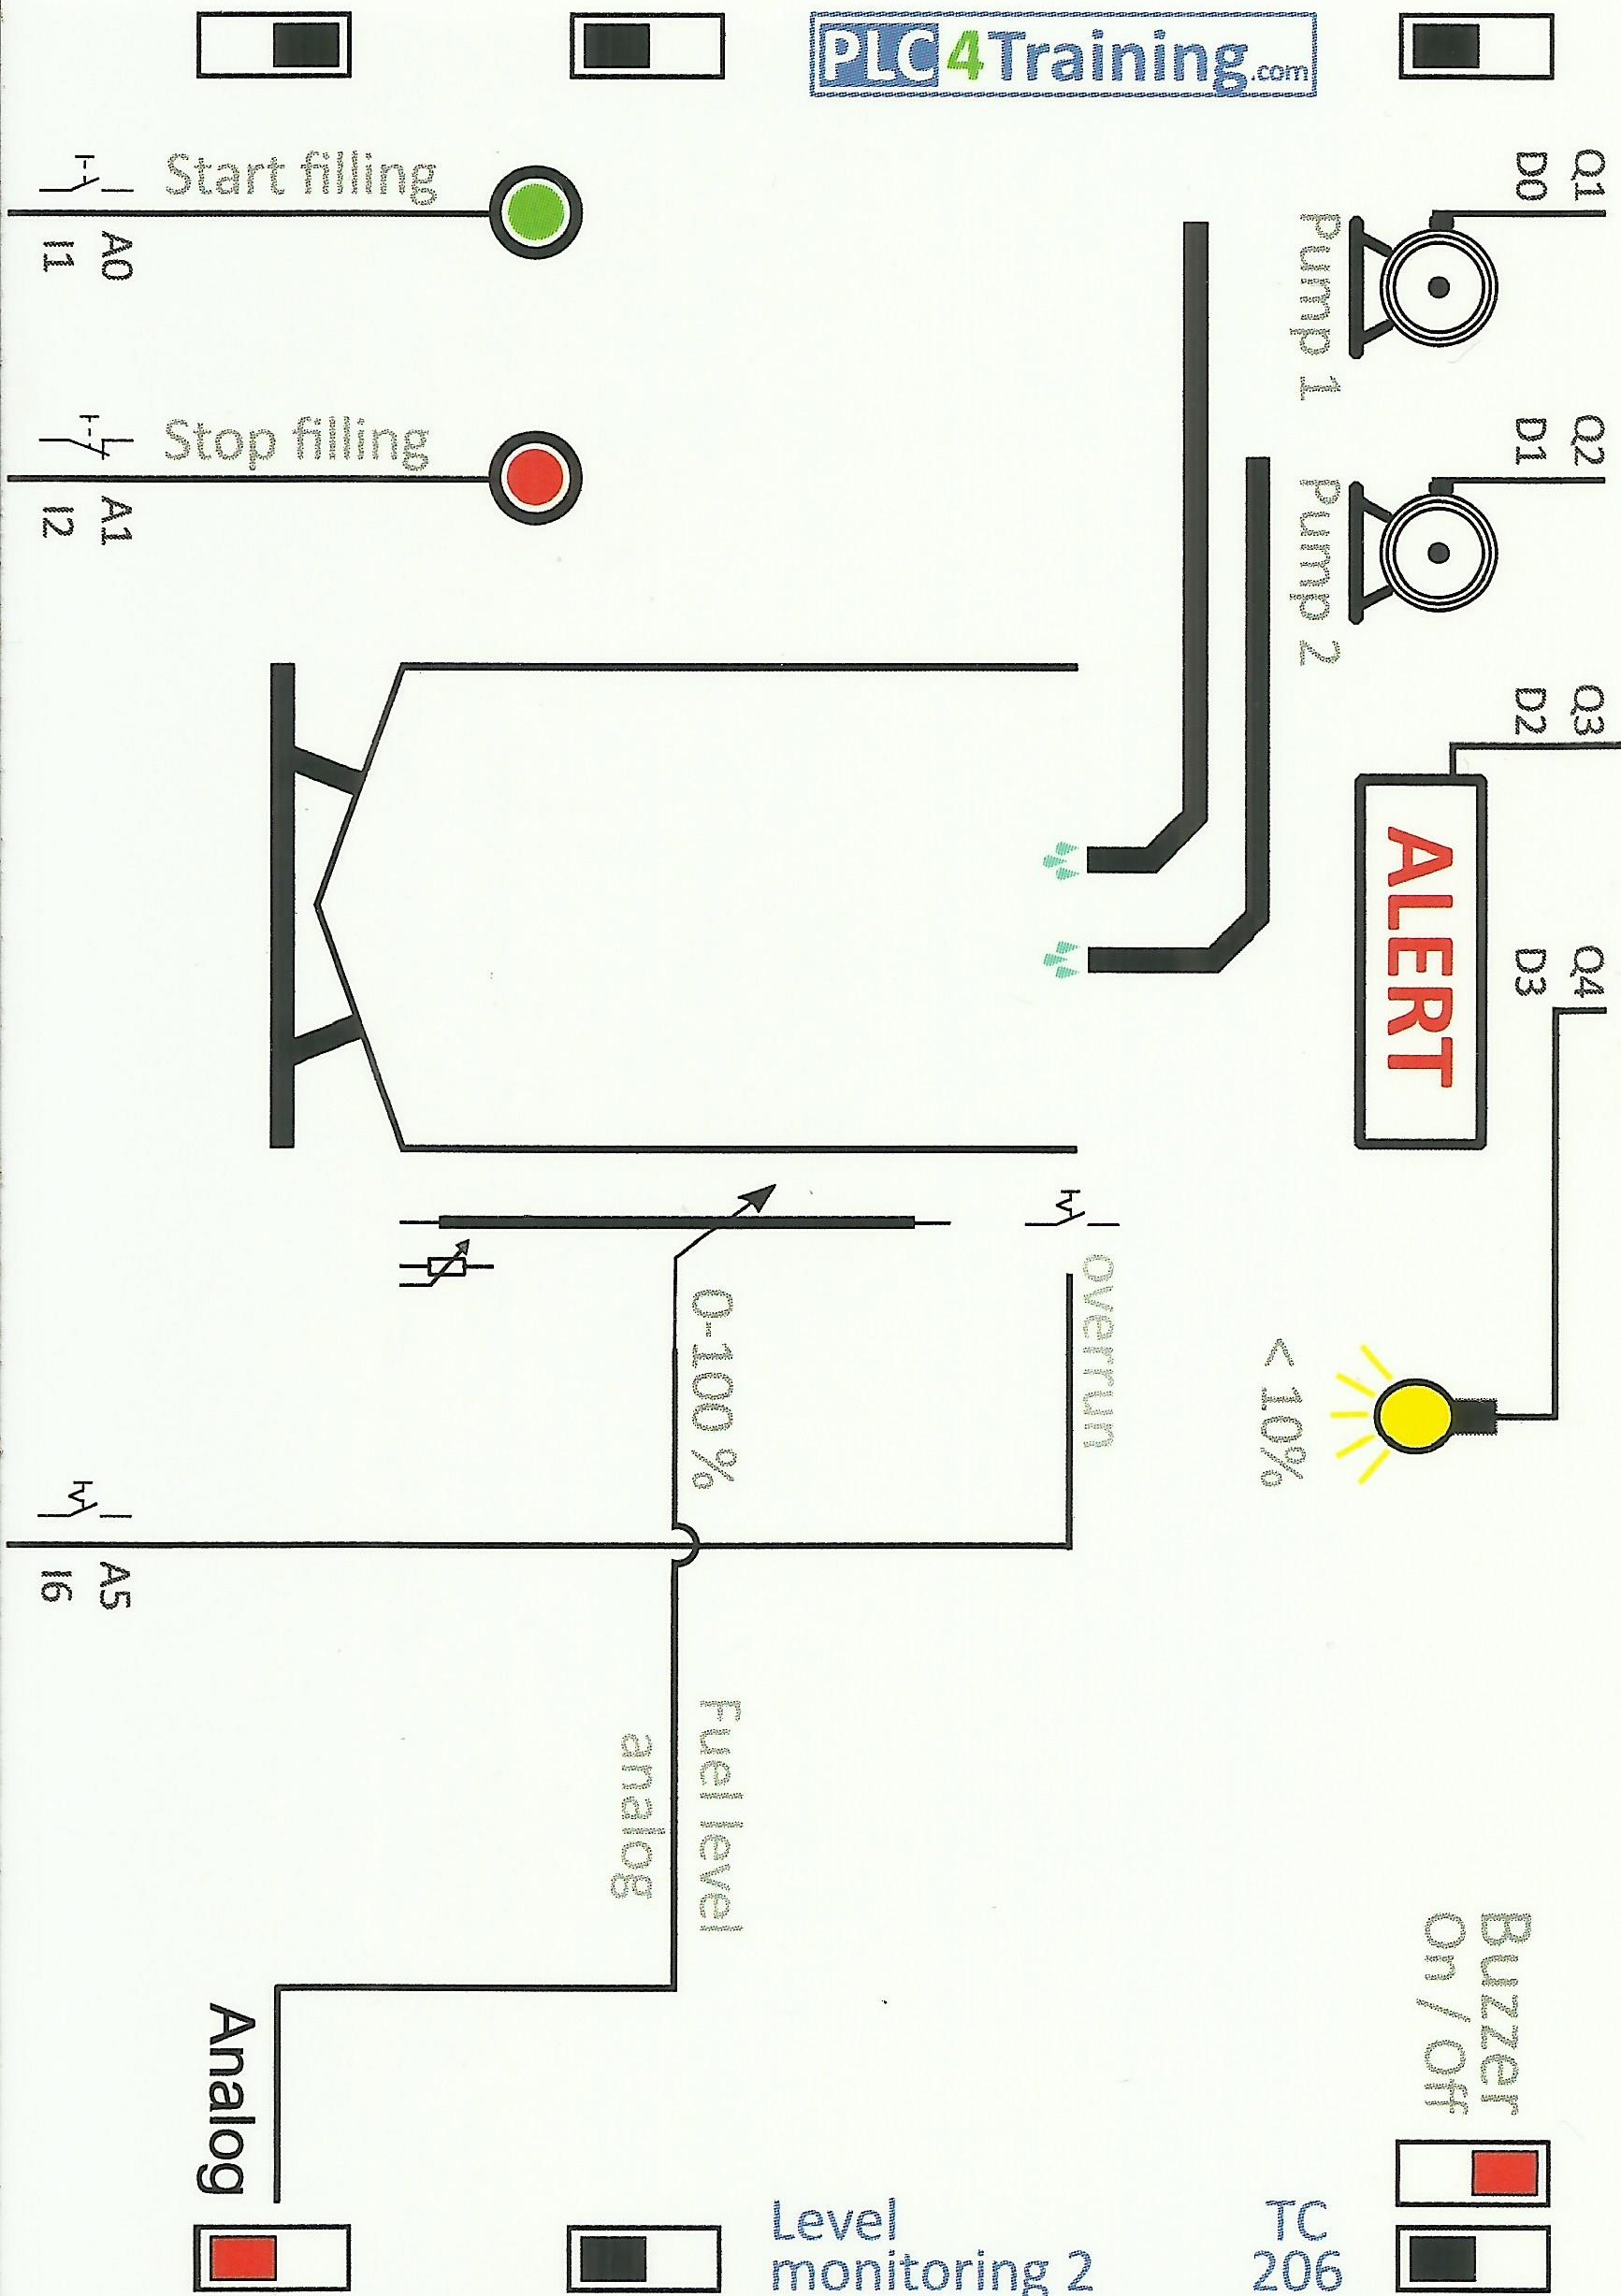
\includegraphics[height=23cm]{206.jpg}}
\captionof{figure}{\texttt{Training Cart 206}}\label{}
\end{center}
\subsubsection{Description du Projet}

Le projet TC 206 a été développé pour simuler le remplissage d'un réservoir à l'aide de deux pompes, avec un émetteur de valeurs analogiques servant de capteur de niveau et un interrupteur à flotteur servant de protection contre le débordement. L'objectif de cette tâche est de fournir une expérience pratique de la mise en œuvre du contrôle du niveau de remplissage d'un réservoir, en utilisant des capteurs analogiques et numériques, ainsi que la gestion des pompes et des alarmes en cas de débordement.

\subsubsection{Tâches Spécifiques}

\begin{enumerate}
    \item \textbf{Surveillance du Niveau avec Capteur Analogique et Interrupteur à Flotteur (Tâche unique):} La tâche implique de démarrer le remplissage du réservoir avec le bouton \(A_0\), pouvant être arrêté à tout moment avec le bouton \(A_1\) (contact normalement fermé). L'émetteur de valeurs analogiques (\(A_7\)) détecte le niveau dans le réservoir. Le remplissage est effectué jusqu'à 80\% avec deux pompes (sorties \(D_0\) et \(D_1\)), puis jusqu'à 100\% avec une seule pompe (sortie \(D_0\)). Si l'interrupteur à flotteur détecte un débordement dans le réservoir, les deux pompes doivent être éteintes. Une alarme est générée à la sortie \(D_2\) jusqu'à ce que l'interrupteur à flotteur ne détecte plus de débordement. Si le niveau dans le réservoir tombe en dessous de 10\%, cela est signalé à la sortie \(D_3\). Un nouveau remplissage du réservoir doit être démarré avec le bouton \(A_0\).
\end{enumerate}

\subsubsection{Capteurs/Actionneurs}

Les composants du projet comprennent des boutons pour les entrées \(A_0\), \(A_1\), l'interrupteur à flotteur pour \(A_5\), l'émetteur de valeurs analogiques pour \(A_7\), ainsi que des sorties \(D_0\), \(D_1\), \(D_2\) et \(D_3\) pour visualiser le fonctionnement des pompes, les alarmes et l'indicateur de niveau. Cette configuration permet aux participants de comprendre la mise en œuvre du contrôle du niveau de remplissage d'un réservoir avec une combinaison de capteurs analogiques et numériques, tout en gérant les pompes et les alarmes associées.

\subsubsection{Code du projet}

\begin{minipage}{0.5\textwidth}
    
\includegraphics[height=3cm]{Code TC206.png}
\end{minipage}%
\begin{minipage}{0.5\textwidth}
    Cliquez sur \href{https://github.com/DexterTaha/Controllino-PLC-Sample/blob/main/TC200/TC206_Surveillance_de_niveau_2/TC206_Surveillance_de_niveau_2.ino}{Code} pour obtenir le code.
\end{minipage}

%TC207\_Display--------------------------------------------------------------------------
\newpage
\subsection{TC207\_Display}
\begin{center}
\rotatebox[origin=c]{360}{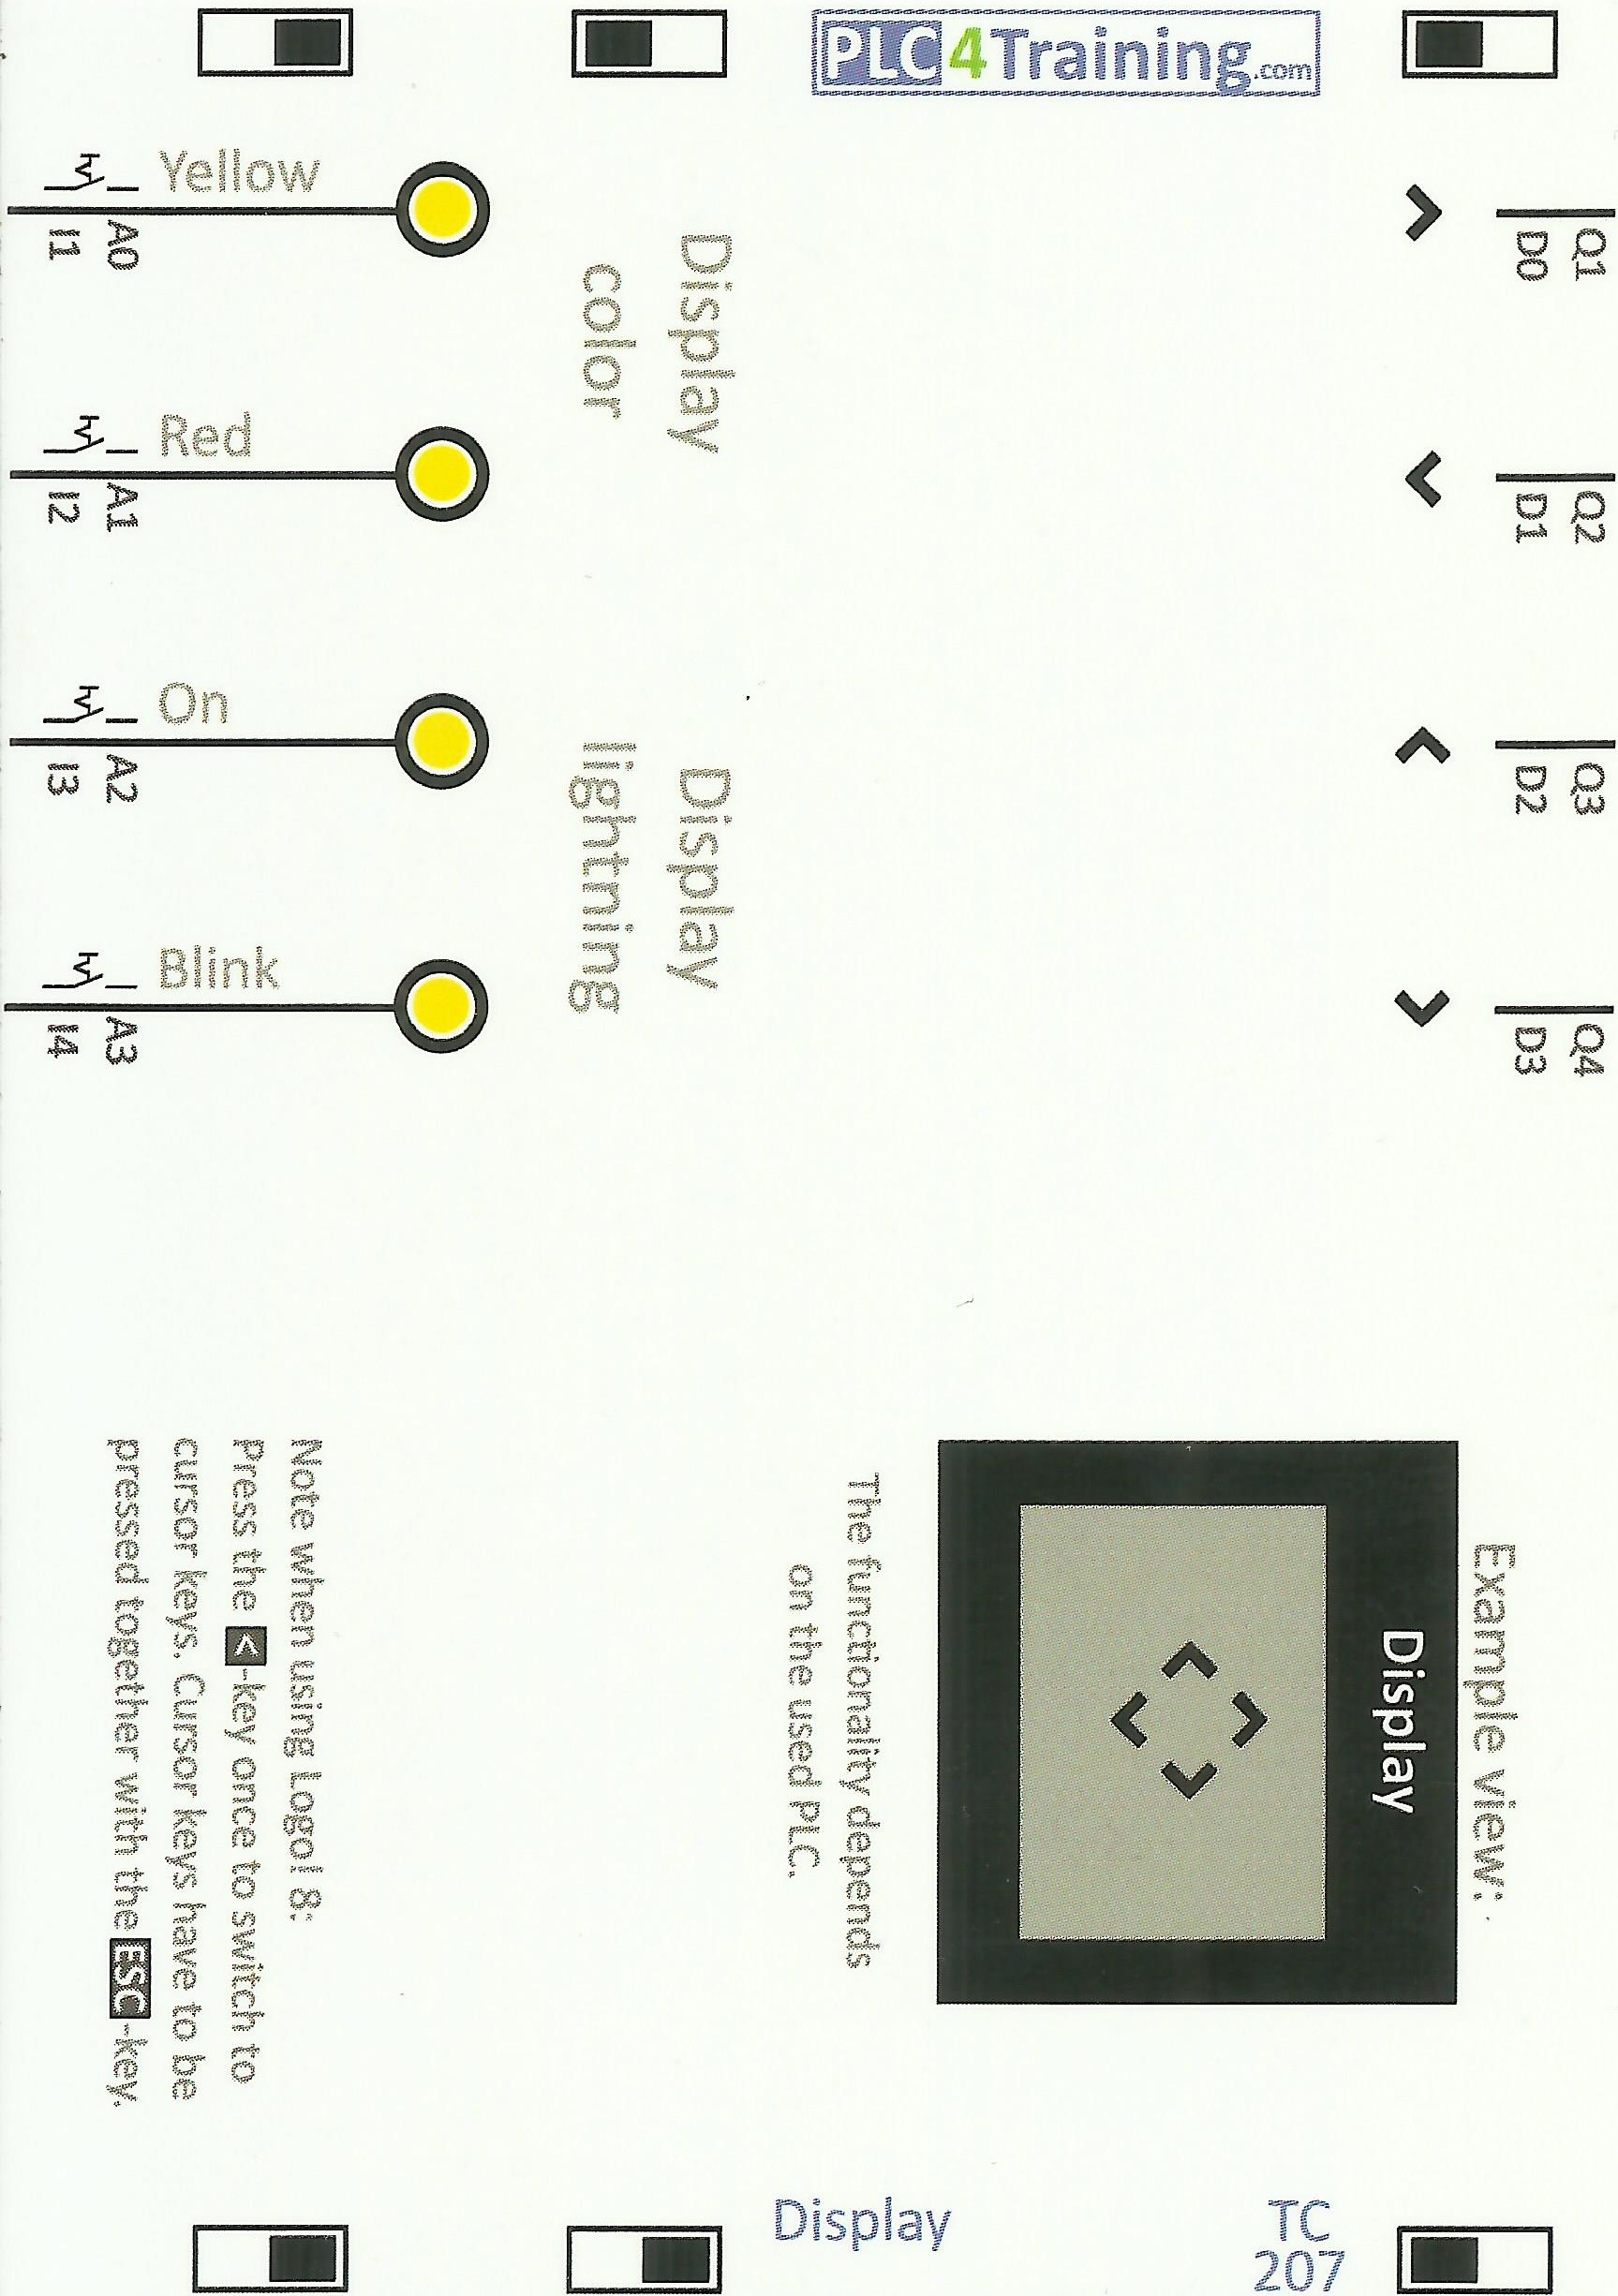
\includegraphics[height=23cm]{207.jpg}}
\captionof{figure}{\texttt{Training Cart 207}}\label{}
\end{center}
\subsubsection{Description du Projet}

Le Controllino n'a pas d'affichage interne. La tâche ne peut donc pas être réalisée.

\subsubsection{Code du projet}

\begin{minipage}{0.5\textwidth}
    
\includegraphics[height=3cm]{Code TC207.png}
\end{minipage}%
\begin{minipage}{0.5\textwidth}
    Cliquez sur \href{https://github.com/DexterTaha/Controllino-PLC-Sample/blob/main/TC200/TC207_Display/TC207_Display.ino}{Code} pour obtenir le code.
\end{minipage}

%TC208\_Valeur\_analogique--------------------------------------------------------------------------
\newpage
\subsection{TC208\_Valeur\_analogique}
\begin{center}
\rotatebox[origin=c]{360}{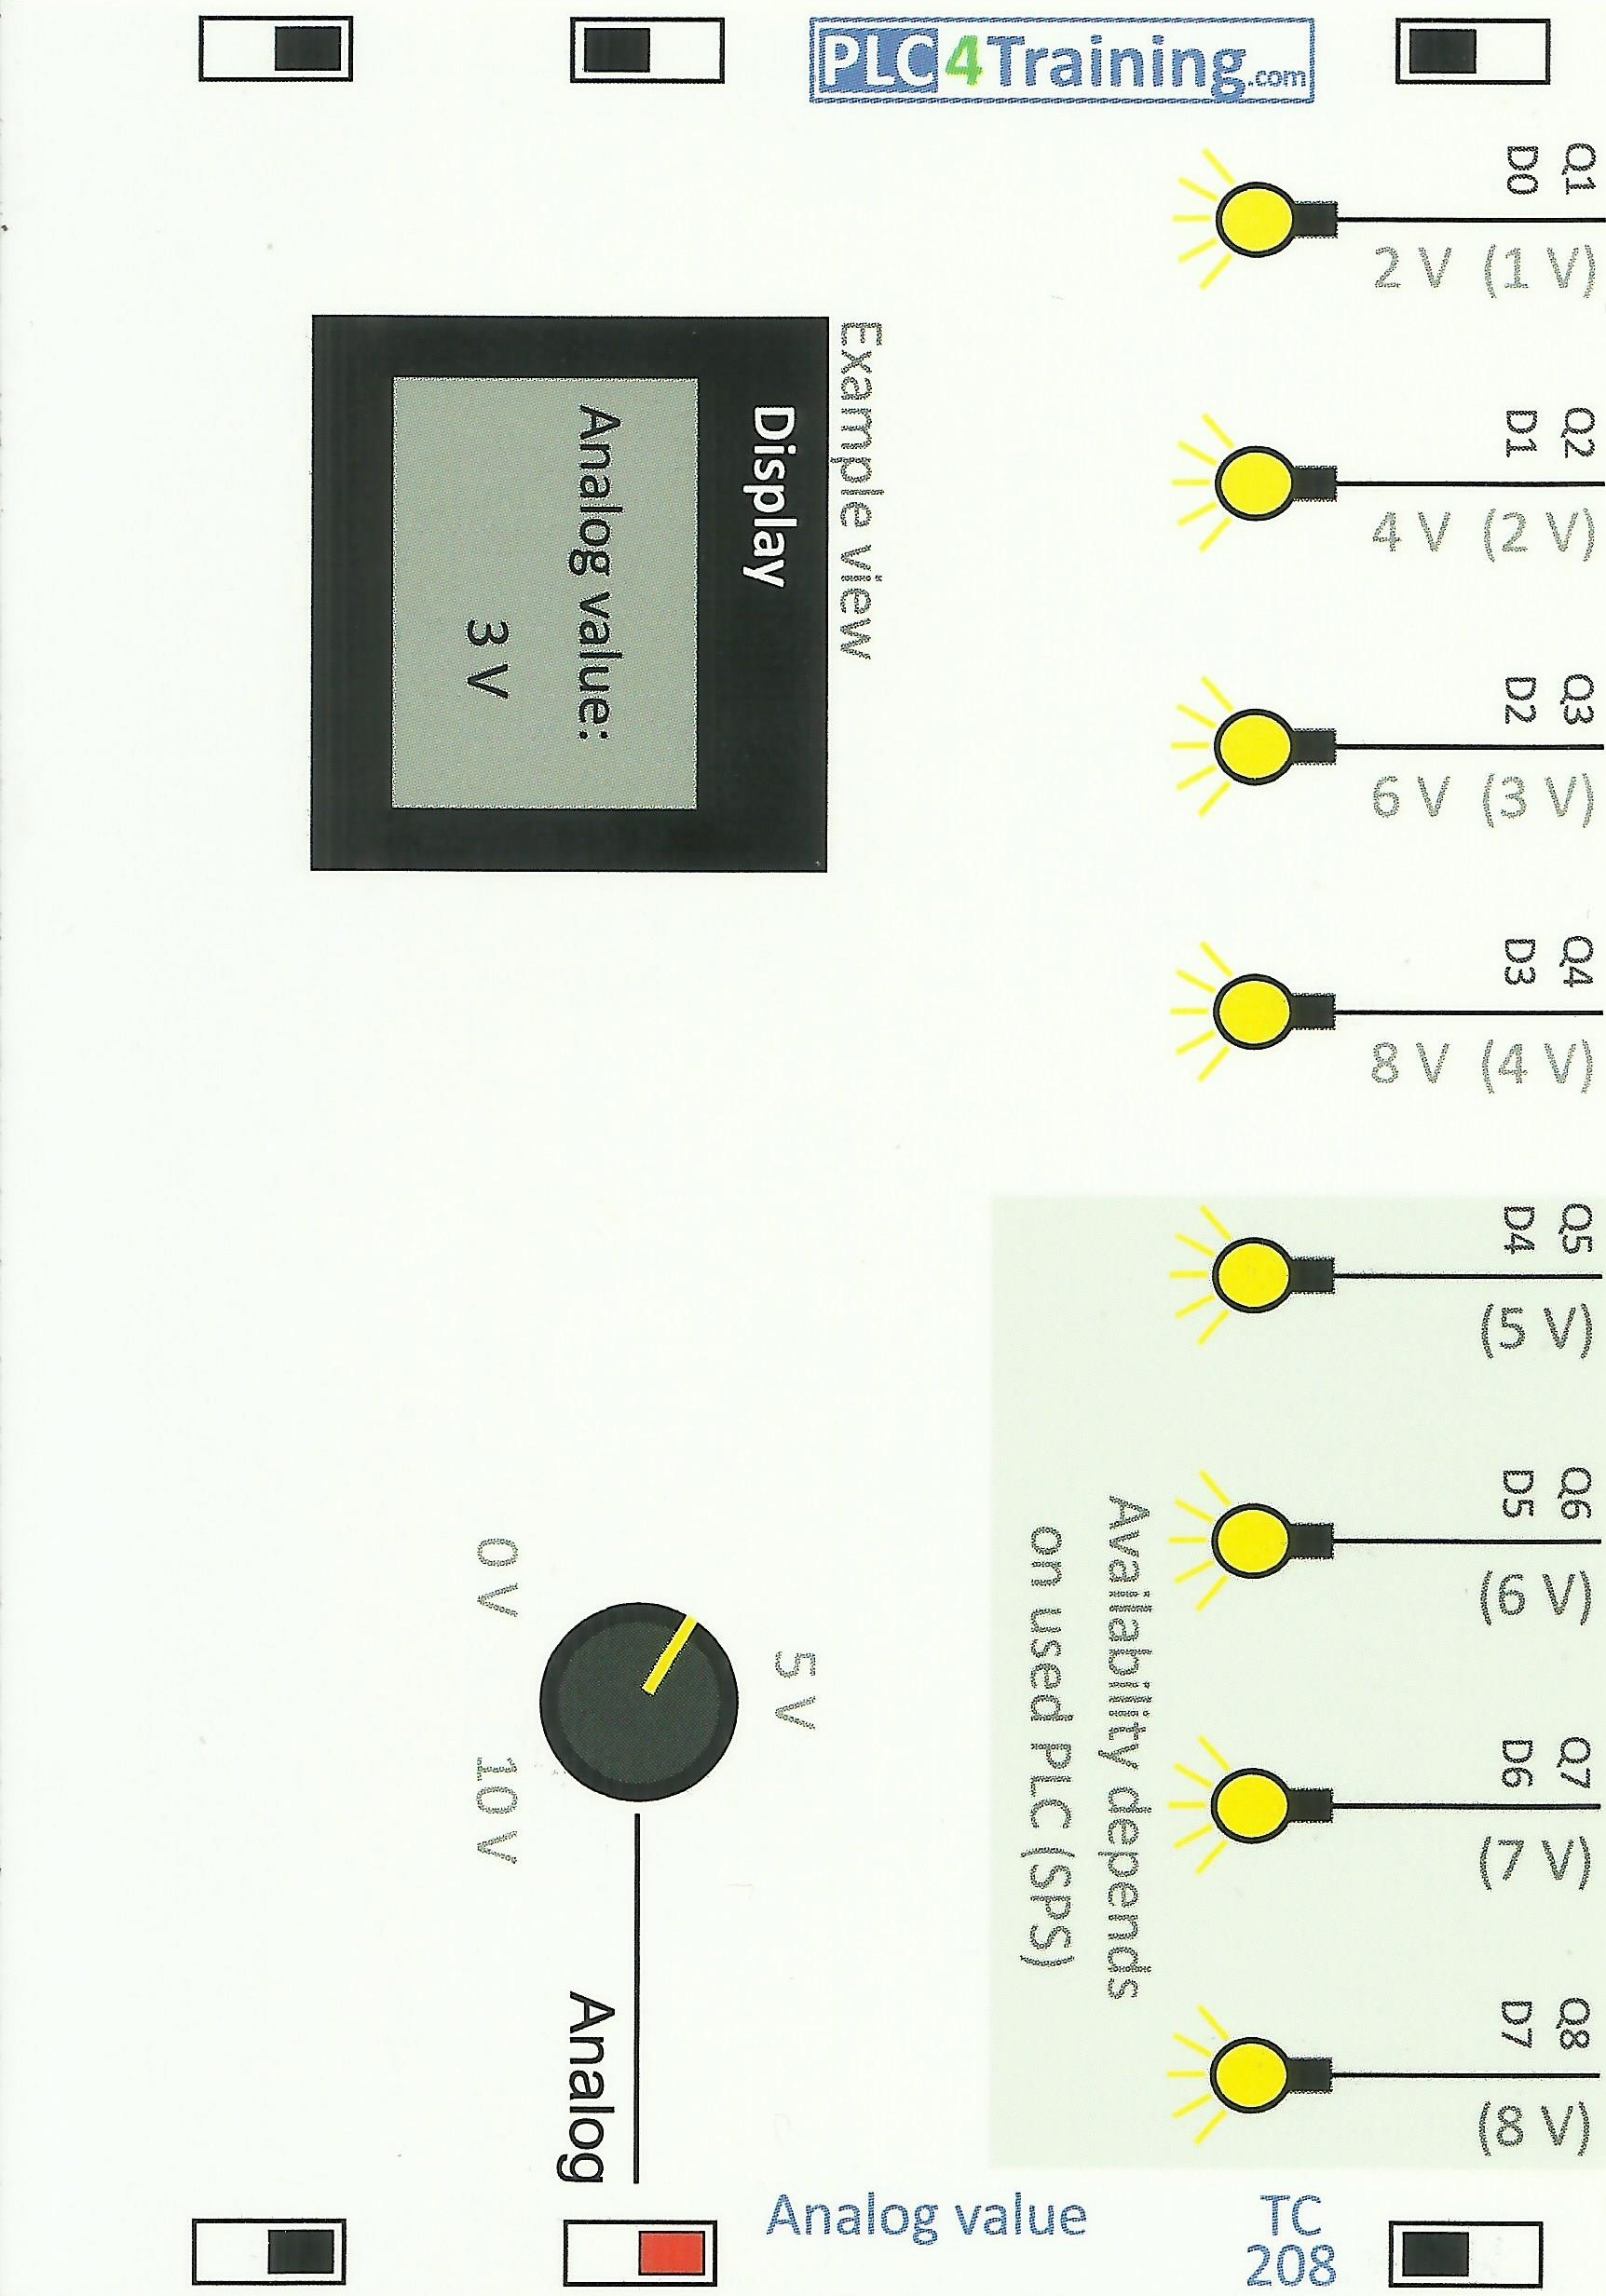
\includegraphics[height=23cm]{208.jpg}}
\captionof{figure}{\texttt{Training Cart 208}}\label{}
\end{center}
\subsubsection{Description du Projet}

Le projet TC 208 a été développé dans le but d'afficher une valeur analogique sur une rangée de LEDs (bande lumineuse LED) à l'aide du Controllino. La tâche consiste à lire une valeur analogique comprise entre 0 et 10 volts à partir de l'entrée \(A_6\) et à signaler cette valeur en activant des LEDs sur les sorties spécifiées. Chaque sortie est activée en fonction de seuils de tension spécifiques.

\subsubsection{Tâches Spécifiques}

La tâche implique la configuration de seuils de tension sur les sorties \(D_0\) à \(D_7\) pour signaler la valeur analogique. Chaque sortie est activée à partir d'une tension spécifique, ce qui permet une visualisation claire de la plage de valeurs analogiques.
\subsubsection{Capteurs/Actionneurs}

Les composants du projet comprennent l'entrée \(A_6\) pour la valeur analogique et les sorties \(D_0\) à \(D_7\) pour signaler la valeur analogique en fonction des seuils spécifiés. Cette configuration permet aux participants de comprendre la mise en œuvre du contrôle d'une valeur analogique et de son affichage à l'aide de LEDs.

\subsubsection{Code du projet}

\begin{minipage}{0.5\textwidth}
    \includegraphics[height=3cm]{Code TC208.png}
\end{minipage}%
\begin{minipage}{0.5\textwidth}
    Cliquez sur \href{https://github.com/DexterTaha/Controllino-PLC-Sample/blob/main/TC200/TC208_Valeur_analogique/TC208_Valeur_analogique.ino}{Code} pour obtenir le code.
\end{minipage}

%TC209\_Compteur\_Rapide--------------------------------------------------------------------------
\newpage
\subsection{TC209\_Compteur\_Rapide}
\begin{center}
\rotatebox[origin=c]{360}{\includegraphics[height=23cm]{209.jpg}}
\captionof{figure}{\texttt{Training Cart 209}}\label{}
\end{center}
\subsubsection{Description du Projet}

Le projet TC 209 a été conçu pour enregistrer le nombre d'impulsions par seconde à l'aide de l'entrée d'interruption du Controllino et afficher ce nombre sur une rangée de LEDs (bande lumineuse LED). La tâche consiste à enregistrer le nombre d'impulsions par seconde à partir de l'entrée d'interruption \(A_3\) / IN0 et à activer des LEDs sur les sorties spécifiées en fonction de seuils de fréquence.

\subsubsection{Tâches Spécifiques}

La tâche implique la configuration de seuils de fréquence sur les sorties \(D_0\) à \(D_7\) pour activer les LEDs en fonction du nombre d'impulsions par seconde enregistrées. Chaque sortie est activée à partir d'un seuil de fréquence spécifique, permettant une visualisation claire de la fréquence des impulsions.

\subsubsection{Capteurs/Actionneurs}

Les composants du projet comprennent l'entrée d'interruption IN0 / \(A_3\) pour le générateur d'impulsions et les sorties \(D_0\) à \(D_7\) pour activer les LEDs en fonction des seuils de fréquence spécifiés. Cette configuration permet aux participants de comprendre la mise en œuvre de la comptabilisation rapide d'impulsions et de la visualisation de la fréquence correspondante.

\subsubsection{Code du projet}

\begin{minipage}{0.5\textwidth}
    \includegraphics[height=3cm]{Code TC209.png}
\end{minipage}%
\begin{minipage}{0.5\textwidth}
    Cliquez sur \href{https://github.com/DexterTaha/Controllino-PLC-Sample/blob/main/TC200/TC209_Compteur_Rapide/TC209_Compteur_Rapide.ino}{Code} pour obtenir le code.
\end{minipage}

%TC210\_Modulation\_de\_Durée\_d'Impulsion--------------------------------------------------------------------------
\newpage
\subsection{TC210\_Modulation\_de\_Durée\_d'Impulsion}
\begin{center}
\rotatebox[origin=c]{360}{\includegraphics[height=23cm]{210.jpg}}
\captionof{figure}{\texttt{Training Cart 210}}\label{}
\end{center}
\subsubsection{Description du Projet}

Le projet TC 210 a été développé dans le but de configurer un feu clignotant avec une durée d'impulsion et une durée de pause d'impulsion variables. La tâche consiste à rendre chaque durée ajustable à l'aide de valeurs analogiques. L'entrée \(A_0\) doit contrôler la sortie \(D_3\) pour simuler un feu clignotant, et la durée de l'impulsion ainsi que la durée de la pause entre les impulsions doivent être réglables avec les valeurs analogiques \(A_6\) et \(A_7\) respectivement.

\subsubsection{Tâches Spécifiques}

La tâche implique la configuration d'un feu clignotant dont la durée de l'impulsion et la durée de la pause entre les impulsions sont ajustables. L'entrée \(A_0\) est utilisée pour activer le feu clignotant, tandis que les valeurs analogiques \(A_6\) et \(A_7\) sont utilisées pour régler respectivement la durée de l'impulsion (\(T_H\)) et la durée de la pause (\(T_L\)).

\subsubsection{Capteurs/Actionneurs}

Les composants du projet comprennent l'entrée \(A_0\) pour activer le feu clignotant, les entrées analogiques \(A_6\) et \(A_7\) pour régler les durées de l'impulsion et de la pause, respectivement, ainsi que la sortie \(D_3\) pour visualiser le feu clignotant. Cette configuration permet aux participants de comprendre la mise en œuvre de la modulation de la durée des impulsions.

\subsubsection{Code du projet}

\begin{minipage}{0.5\textwidth}
    \includegraphics[height=3cm]{Code TC210.png}
\end{minipage}%
\begin{minipage}{0.5\textwidth}
    Cliquez sur \href{https://github.com/DexterTaha/Controllino-PLC-Sample/blob/main/TC200/TC210_Modulation_de_Dur%C3%A9e_d'Impulsion/TC210_Modulation_de_Dur%C3%A9e_d'Impulsion.ino}{Code} pour obtenir le code.
\end{minipage}

%TC211\_Escalator--------------------------------------------------------------------------
\newpage
\subsection{TC211\_Escalator}
\begin{center}
\rotatebox[origin=c]{360}{\includegraphics[height=23cm]{211.jpg}}
\captionof{figure}{\texttt{Training Cart 211}}\label{}
\end{center}
\subsubsection{Description du Projet}

Le projet TC 211 a été développé dans le but de simuler un escalier roulant. La tâche consiste à activer et désactiver l'escalier roulant via un interrupteur (entrée \(A_0\)). Le moteur de l'escalier roulant est contrôlé par la sortie \(D_3\). Un capteur de barrière lumineuse à l'entrée \(A_2\) au bas de l'escalier roulant active le moteur pendant 10 secondes, après quoi il s'arrête à nouveau. En cas d'arrêt d'urgence (interrupteur d'arrêt d'urgence à l'entrée \(A_1\) ou \(A_7\)) ou si le capteur (entrée \(A_6\)) signale une courroie cassée, le moteur est immédiatement éteint, et une alarme est émise. Le bouton à l'entrée \(A_4\) réinitialise cette défaillance après qu'elle a été résolue.

\subsubsection{Tâches Spécifiques}

La tâche implique la simulation d'un escalier roulant avec un ensemble de fonctionnalités spécifiques :
\begin{itemize}
    \item Activation/désactivation de l'escalier roulant avec un interrupteur (\(A_0\)).
    \item Contrôle du moteur de l'escalier roulant avec la sortie \(D_3\).
    \item Activation du moteur par un capteur de barrière lumineuse pendant 10 secondes.
    \item Arrêt d'urgence immédiat en cas d'activation d'un interrupteur d'arrêt d'urgence (\(A_1\) ou \(A_7\)) ou en cas de détection d'une courroie cassée (\(A_6\)).
    \item Émission d'une alarme visuelle et sonore en cas d'arrêt d'urgence ou de détection d'une courroie cassée.
    \item Réinitialisation de la défaillance avec un bouton après résolution du problème.
\end{itemize}

\subsubsection{Capteurs/Actionneurs}

Les composants du projet comprennent des entrées pour l'interrupteur de l'escalier roulant (\(A_0\)), l'arrêt d'urgence (\(A_1\) ou \(A_7\)), la barrière lumineuse (\(A_2\)), le bouton de réinitialisation d'alarme (\(A_4\)) et le capteur de courroie cassée (\(A_6\)). Les sorties incluent la visualisation de l'escalier roulant (\(D_0\)), l'alarme visuelle/sonore (\(D_2\)) et le contrôle du moteur (\(D_3\)). Cette configuration permet aux participants de comprendre la mise en œuvre de la simulation d'un escalier roulant avec des fonctionnalités de sécurité et de contrôle.

\subsubsection{Code du projet}

\begin{minipage}{0.5\textwidth}
    \includegraphics[height=3cm]{Code TC211.png}
\end{minipage}%
\begin{minipage}{0.5\textwidth}
    Cliquez sur \href{https://github.com/DexterTaha/Controllino-PLC-Sample/blob/main/TC200/TC211_Escalator/TC211_Escalator.ino}{Code} pour obtenir le code.
\end{minipage}

%TC300--------------------------------------------------------------------------
\newpage
\section{TC300}

Niveau de difficulté 300 :\\

Les tâches et les cartes de formation du niveau 300 contiennent des tâches complexes. Une esquisse de la tâche peut être programmée dans l'IDE Arduino IDE avec de nombreuses lignes de code. Une solution pour cette tâche peut prendre plusieurs heures ou plusieurs jours. Les tâches et les Les tâches et les cartes de formation sont marquées comme suit : TC 300, TC 301, TC 302, etc.

%TC300\_Parking--------------------------------------------------------------------------
\newpage
\subsection{TC300\_Parking}
\begin{center}
\rotatebox[origin=c]{360}{\includegraphics[height=23cm]{300.jpg}}
\captionof{figure}{\texttt{Training Cart 300}}\label{}
\end{center}
\subsubsection{Description du Projet}

Le projet TC 300 a été développé dans le but de contrôler les feux de signalisation pour un parking à plusieurs étages avec 20 places de stationnement. Le contrôle des feux de signalisation à l'entrée doit indiquer si des places de stationnement sont encore disponibles. Le compteur interne des places de stationnement doit être manuellement modifiable en cas de comptage défectueux.

\subsubsection{Tâches Spécifiques}

La tâche implique la mise en place d'un système de contrôle de feux de signalisation pour un parking à plusieurs étages avec les fonctionnalités suivantes :
\begin{itemize}
    \item Utilisation de barrières lumineuses à l'entrée (\(A_0\)) et à la sortie (\(A_7\)) pour enregistrer le nombre de véhicules dans le parking.
    \item Changement des feux de signalisation à l'entrée en fonction de l'occupation du parking (feu vert si des places sont disponibles, feu rouge si le parking est complet).
    \item Possibilité de réinitialiser manuellement le compteur des places de stationnement (\(A_1\)).
    \item Possibilité d'ajuster manuellement le compteur des places de stationnement (\(A_2\)).
\end{itemize}
Le code \texttt{TC300\_Parking.ino} fournit une solution complète pour cette tâche.

\subsubsection{Capteurs/Actionneurs}

Les composants du projet comprennent des entrées pour les barrières lumineuses à l'entrée (\(A_0\)) et à la sortie (\(A_7\)), ainsi que des boutons pour réinitialiser le compteur (\(A_1\)) et ajuster manuellement le compteur (\(A_2\)). Les sorties comprennent la visualisation des feux de signalisation à l'entrée (\(D_0\) et \(D_1\)). Cette configuration permet aux participants de comprendre la mise en œuvre du contrôle de feux de signalisation pour un parking avec gestion du compteur des places de stationnement.

\subsubsection{Code du projet}

\begin{minipage}{0.5\textwidth}
    \includegraphics[height=3cm]{Code TC300.png}
\end{minipage}%
\begin{minipage}{0.5\textwidth}
    Cliquez sur \href{https://github.com/DexterTaha/Controllino-PLC-Sample/blob/main/TC300/TC300_Parking/TC300_Parking.ino}{Code} pour obtenir le code.
\end{minipage}

%TC301\_Lumière\_clignotante--------------------------------------------------------------------------
\newpage
\subsection{TC301\_Lumière\_clignotante}
\begin{center}
\rotatebox[origin=c]{360}{\includegraphics[height=23cm]{301.jpg}}
\captionof{figure}{\texttt{Training Cart 301}}\label{}
\end{center}
\subsubsection{Description du Projet}

Le projet TC 301 a été développé dans le but de mettre en place des balises lumineuses pour protéger un chantier de construction. Les lumières des balises doivent s'allumer l'une après l'autre, et la direction de la lumière en mouvement doit être commutable.

\subsubsection{Tâches Spécifiques}

La tâche consiste à configurer des balises lumineuses pour avertir et protéger un chantier de construction. Les fonctionnalités spécifiques comprennent :
\begin{itemize}
    \item Activation du feu de signalisation en mouvement avec un interrupteur (\(A_0\)).
    \item Allumage successif des sorties \(D_0\) à \(D_3\), représentant les balises lumineuses.
    \item Possibilité de changer la direction de la lumière en mouvement avec un interrupteur (\(A_1\)).
\end{itemize}
Le code \texttt{TC301\_Lumière\_clignotante.ino} fournit une solution complète pour cette tâche.

\subsubsection{Capteurs/Actionneurs}

Les composants du projet comprennent un interrupteur pour démarrer la lumière en mouvement (\(A_0\)), un interrupteur pour sélectionner la rotation à gauche ou à droite (\(A_1\)), et des sorties pour visualiser les balises lumineuses (\(D_0\) à \(D_3\)). Cette configuration permet aux participants de comprendre la mise en œuvre d'un système de balises lumineuses avec la possibilité de changer la direction du mouvement.

\subsubsection{Code du projet}

\begin{minipage}{0.5\textwidth}
    \includegraphics[height=3cm]{Code TC301.png}
\end{minipage}%
\begin{minipage}{0.5\textwidth}
    Cliquez sur \href{https://github.com/DexterTaha/Controllino-PLC-Sample/blob/main/TC300/TC301_Lumi%C3%A8re_clignotante/TC301_Lumi%C3%A8re_clignotante.ino}{Code} pour obtenir le code.
\end{minipage}

%TC302\_Compteur--------------------------------------------------------------------------
\newpage
\subsection{TC302\_Compteur}
\begin{center}
\rotatebox[origin=c]{360}{\includegraphics[height=23cm]{302.jpg}}
\captionof{figure}{\texttt{Training Cart 302}}\label{}
\end{center}
\subsubsection{Description du Projet}

Le projet TC 302 a été développé dans le but de permettre l'allumage et l'extinction individuels des LEDs d'une rangée de LEDs (bande lumineuse à LED). Trois boutons sont utilisés pour réaliser les fonctions "Allumer une LED", "Éteindre une LED" ou "Éteindre toutes les LEDs".

\subsubsection{Tâches Spécifiques}

La tâche consiste à contrôler individuellement les LEDs d'une rangée de LEDs (\(D_0\) à \(D_3\)) avec les fonctionnalités suivantes :
\begin{itemize}
    \item Allumage d'une LED avec le bouton (\(A_0\)).
    \item Extinction d'une LED avec le bouton (\(A_1\)).
    \item Extinction de toutes les LEDs avec le bouton (\(A_2\)).
\end{itemize}
Le code \texttt{TC302\_Compteur.ino} fournit une solution complète pour cette tâche.

\subsubsection{Capteurs/Actionneurs}

Les composants du projet comprennent des boutons pour allumer une LED (\(A_0\)), éteindre une LED (\(A_1\)), et éteindre toutes les LEDs (\(A_2\)), ainsi que des sorties pour visualiser les LEDs individuelles (\(D_0\) à \(D_3\)). Cette configuration permet aux participants de comprendre la mise en œuvre du contrôle individuel des LEDs dans une rangée.

\subsubsection{Code du projet}

\begin{minipage}{0.5\textwidth}
    \includegraphics[height=3cm]{Code TC202.png}
\end{minipage}%
\begin{minipage}{0.5\textwidth}
    Cliquez sur \href{https://github.com/DexterTaha/Controllino-PLC-Sample/blob/main/TC300/TC302_Compteur/TC302_Compteur.ino}{Code} pour obtenir le code.
\end{minipage}

%TC303\_Grue--------------------------------------------------------------------------
\newpage
\subsection{TC303\_Grue}
\begin{center}
\rotatebox[origin=c]{360}{\includegraphics[height=23cm]{303.jpg}}
\captionof{figure}{\texttt{Training Cart 303}}\label{}
\end{center}
\subsubsection{Description du Projet}

Le projet TC 303 a été développé dans le but de simuler le contrôle d'une grue avec surveillance de charge. La mise en œuvre comprend le démarrage/arrêt de la grue, la levée et la descente de la charge, la détection de la position du treuil, la surveillance de la charge, l'arrêt d'urgence, et la réinitialisation de l'alarme.

\subsubsection{Tâches Spécifiques}

La tâche spécifique consiste en :
\begin{itemize}
    \item Allumage/arrêt de la grue avec l'interrupteur (\(A_0\)), signalé à la sortie \(D_3\).
    \item Levée de la charge avec le bouton (\(A_1\)) et descente avec le bouton (\(A_2\)).
    \item Contrôle du moteur du treuil avec les sorties \(D_0\) "Lever la charge" et \(D_1\) "Abaisser la charge".
    \item Détection de la position du treuil avec le capteur (\(A_3\)), entraînant l'arrêt immédiat du processus de levage s'il est en haut.
    \item Surveillance de la charge avec le capteur analogique (\(A_7\)), avec une interruption du processus de levage et déclenchement d'une alarme (\(D_2\)) si la charge est de 600 kg ou plus.
    \item Arrêt d'urgence avec le bouton (\(A_5\)), arrêtant immédiatement tous les mouvements de la grue.
    \item Indication de l'alarme à la sortie \(D_2\), avec possibilité de réinitialisation via le bouton (\(A_4\)).
\end{itemize}

\subsubsection{Capteurs/Actionneurs}

Les composants du projet comprennent un interrupteur pour allumer/éteindre la grue (\(A_0\)), des boutons pour lever (\(A_1\)) et abaisser (\(A_2\)) la charge, un capteur pour détecter la position du treuil (\(A_3\)), un bouton d'arrêt d'urgence (\(A_5\)), un capteur de charge (\(A_7\)), et des sorties pour contrôler le moteur du treuil (\(D_0\) et \(D_1\)) ainsi que pour signaler l'état de la grue (\(D_3\)) et l'alarme (\(D_2\)).

\subsubsection{Code du projet}

\begin{minipage}{0.5\textwidth}
    \includegraphics[height=3cm]{Code TC303.png}
\end{minipage}%
\begin{minipage}{0.5\textwidth}
    Cliquez sur \href{https://github.com/DexterTaha/Controllino-PLC-Sample/blob/main/TC300/TC303_Grue/TC303_Grue.ino}{Code} pour obtenir le code.
\end{minipage}

%TC304\_Ligne\_d'assemblage--------------------------------------------------------------------------
\newpage
\subsection{TC304\_Ligne\_d'assemblage}
\begin{center}
\rotatebox[origin=c]{360}{\includegraphics[height=23cm]{304.jpg}}
\captionof{figure}{\texttt{Training Cart 304}}\label{}
\end{center}
\subsubsection{Description du Projet}

Le projet TC 304 a été développé dans le but de simuler le contrôle d'une ligne de montage ou d'un convoyeur avec une fonction d'arrêt d'urgence. La tâche spécifique consiste à transporter un colis en marche arrière sur un tapis roulant (de gauche à droite et vice versa), avec la mise en œuvre d'une fonction d'arrêt d'urgence pour assurer la sécurité.

\subsubsection{Tâches Spécifiques}

La tâche spécifique comprend les éléments suivants :
\begin{itemize}
    \item Allumage/arrêt du convoyeur avec l'interrupteur (\(A_0\)).
    \item Détection d'un colis entrant avec la barrière lumineuse à gauche (\(A_2\)) et à droite (\(A_6\)).
    \item Contrôle du moteur du tapis roulant avec les sorties \(D_0\) (direction de transport à gauche) et \(D_1\) (direction de transport à droite).
    \item Fonction d'arrêt d'urgence avec le bouton d'arrêt d'urgence (\(A_3\)), entraînant l'arrêt immédiat du tapis roulant et la génération d'une alarme (\(D_2\)).
    \item Réinitialisation de l'alarme avec le bouton (\(A_4\)).
\end{itemize}

\subsubsection{Capteurs/Actionneurs}

Les composants du projet comprennent un interrupteur pour allumer/éteindre le convoyeur (\(A_0\)), des barrières lumineuses pour détecter l'arrivée d'un colis à gauche (\(A_2\)) et à droite (\(A_6\)), un bouton d'arrêt d'urgence (\(A_3\)), un bouton de réinitialisation d'alarme (\(A_4\)), et des sorties pour contrôler le moteur du tapis roulant (\(D_0\) et \(D_1\)) ainsi que pour signaler l'alarme (\(D_2\)).

\subsubsection{Code du projet}

\begin{minipage}{0.5\textwidth}
    \includegraphics[height=3cm]{Code TC304.png}
\end{minipage}%
\begin{minipage}{0.5\textwidth}
    Cliquez sur \href{https://github.com/DexterTaha/Controllino-PLC-Sample/blob/main/TC300/TC304_Ligne_d'assemblage/TC304_Ligne_d'assemblage.ino}{Code} pour obtenir le code.
\end{minipage}

%TC305\_Garage\_de\_stationnement--------------------------------------------------------------------------
\newpage
\subsection{TC305\_Garage\_de\_stationnement}
\begin{center}
\rotatebox[origin=c]{360}{\includegraphics[height=23cm]{305.jpg}}
\captionof{figure}{\texttt{Training Cart 305}}\label{}
\end{center}

\subsubsection{Description du Projet}

Le projet TC 305 a été conçu pour simuler le contrôle d'une porte de garage avec une seule voie d'entrée et de sortie, utilisant un feu de circulation pour sécuriser la direction opposée. L'objectif est de garantir un fonctionnement sécurisé de la porte, en évitant les accidents potentiels lors de l'entrée ou de la sortie d'un véhicule.

\subsubsection{Tâches Spécifiques}

La tâche spécifique implique les étapes suivantes :
\begin{itemize}
    \item Un bouton (\(A_0\)) situé à l'entrée signale la demande d'entrée au PLC.
    \item Avant l'ouverture de la porte, le feu de circulation (\(D_3\)) à l'intérieur du parking est mis au rouge.
    \item La sortie \(D_1\) contrôle le moteur pour ouvrir la porte, et le bouton de fin de course \(A_3\) signale lorsque la porte est complètement ouverte.
    \item La porte reste ouverte pendant 30 secondes avant de se refermer automatiquement.
    \item Avant la fermeture de la porte, le feu de circulation (\(D_0\)) à l'entrée est également mis au rouge.
    \item La sortie \(D_2\) contrôle le moteur pour fermer la porte, et le bouton de fin de course \(A_4\) signale que la porte est complètement fermée.
\end{itemize}
Les mêmes règles s'appliquent pour la sortie, où la demande de sortie est effectuée via le bouton \(A_6\).
Le code \texttt{TC305\_Garage\_de\_stationnement.ino} fournit une solution complète pour cette tâche.

\subsubsection{Capteurs/Actionneurs}

Les composants du projet comprennent un bouton de demande d'entrée (\(A_0\)), des boutons de fin de course pour l'ouverture (\(A_3\)) et la fermeture (\(A_4\)) de la porte, un bouton de demande de sortie (\(A_6\)), des sorties pour contrôler le feu de circulation à l'entrée (\(D_0\), \(D_3\)) et le moteur pour ouvrir/fermer la porte (\(D_1\), \(D_2\)).

\subsubsection{Code du projet}

\begin{minipage}{0.5\textwidth}
    \includegraphics[height=3cm]{Code TC305.png}
\end{minipage}%
\begin{minipage}{0.5\textwidth}
    Cliquez sur \href{https://github.com/DexterTaha/Controllino-PLC-Sample/blob/main/TC300/TC305_Garage_de_stationnement/TC305_Garage_de_stationnement.ino}{Code} pour obtenir le code.
\end{minipage}

%TC306\_Automate\_de\_vides--------------------------------------------------------------------------
\newpage
\subsection{TC306\_Automate\_de\_vides}
\begin{center}
\rotatebox[origin=c]{360}{\includegraphics[height=23cm]{306.jpg}}
\captionof{figure}{\texttt{Training Cart 306}}\label{}
\end{center}

\subsubsection{Description du Projet}

Le projet TC 306 simule le contrôle d'une machine de consigne pour bouteilles de boissons. Ce type de système est couramment utilisé dans de nombreux pays où une consigne est prélevée sur les bouteilles de boissons, et cette consigne est remboursée lorsqu'une bouteille est retournée via une machine automatique.

\subsubsection{Tâches Spécifiques}

La tâche spécifique implique les étapes suivantes :
\begin{itemize}
    \item La machine de consigne est activée avec le commutateur \(A_0\).
    \item Lorsqu'une bouteille est insérée dans la machine, elle est détectée par la barrière lumineuse \(A_1\).
    \item La bouteille est transportée par le tapis roulant 1 (sortie moteur \(D_0\)) jusqu'à ce qu'elle soit détectée par la barrière lumineuse \(A_2\).
    \item Le moteur (\(D_0\)) est arrêté et le scanner de code-barres est activé à la sortie \(D_1\).
    \item Si un code-barres valide est reconnu par le scanner, cela est signalé à l'entrée \(A_3\).
    \item La bouteille est ensuite transportée plus loin par le tapis roulant 2 (sortie moteur \(D_2\)) jusqu'à ce qu'elle soit détectée par la barrière lumineuse \(A_5\).
    \item Le tapis roulant 2 est arrêté et la presse à bouteilles (sortie \(D_3\)) est activée. La presse à bouteilles prend 5 secondes, puis le moteur (\(D_2\)) du tapis roulant 2 est redémarré. Le tapis roulant continue de fonctionner jusqu'à ce que la bouteille pressée ait quitté la barrière lumineuse (\(A_5\)).
\end{itemize}

\subsubsection{Capteurs/Actionneurs}

Les composants du projet comprennent un commutateur pour activer la machine (\(A_0\)), des boutons pour les barrières lumineuses (\(A_1\), \(A_2\), \(A_5\)) et le scanner de code-barres (\(A_3\)), des sorties pour les moteurs de tapis roulant (\(D_0\), \(D_2\)) et la presse à bouteilles (\(D_3\)), et une sortie pour le scanner de code-barres (\(D_1\)).

\subsubsection{Code du projet}

\begin{minipage}{0.5\textwidth}
    \includegraphics[height=3cm]{Code TC306.png}
\end{minipage}%
\begin{minipage}{0.5\textwidth}
    Cliquez sur \href{https://github.com/DexterTaha/Controllino-PLC-Sample/blob/main/TC300/TC306_Automate_de_vides/TC306_Automate_de_vides.ino}{Code} pour obtenir le code.
\end{minipage}

%TC307\_Chauffage--------------------------------------------------------------------------
\newpage
\subsection{TC307\_Chauffage}
\begin{center}
\rotatebox[origin=c]{360}{\includegraphics[height=23cm]{307.jpg}}
\captionof{figure}{\texttt{Training Cart 307}}\label{}
\end{center}
\subsubsection{Description du Projet}

Le projet TC 307 simule le contrôle d'un système de chauffage, mettant particulièrement l'accent sur la charge de la chaudière d'eau chaude. Cela correspond au fonctionnement typique d'un système de chauffage conventionnel dans les bâtiments résidentiels et commerciaux, où la chaleur est générée par la combustion de combustibles tels que le pétrole, le gaz ou les granulés.

\subsubsection{Tâches Spécifiques}

La tâche spécifique de ce projet est la suivante :
\begin{itemize}
    \item Le système de chauffage est activé ou désactivé de manière centralisée avec le commutateur à l'entrée \(A_0\).
    \item L'opération de chauffage est signalée à la sortie \(D_0\).
    \item La production d'eau chaude est gérée par le brûleur, contrôlé par la sortie \(D_1\). Le processus de chauffage démarre dès que la température dans la chaudière (mesurée à l'aide du capteur \(A_7\)) descend en dessous de 60°C. Le brûleur s'éteint lorsque la température atteint 80°C.
    \item Pour des raisons de sécurité, la chaudière est équipée d'un interrupteur de température excessive (réalisé sous forme d'un contact normalement fermé) connecté à l'entrée \(A_3\). En cas de température excessive, le brûleur doit être immédiatement désactivé, et une alarme est générée à la sortie \(D_2\).
    \item Après la résolution du problème de température excessive, l'alarme peut être réinitialisée manuellement via le bouton-poussoir à l'entrée \(A_4\). Jusqu'à ce que cela soit fait, le brûleur doit rester désactivé de manière sécurisée.
\end{itemize}
Le code \texttt{TC307\_Chauffage.ino} fournit une solution complète pour cette tâche.

\subsubsection{Capteurs/Actionneurs}

Les composants principaux de ce projet incluent un commutateur pour activer le système de chauffage (\(A_0\)), un bouton pour l'interrupteur de température excessive (\(A_3\)), un bouton pour la réinitialisation de l'alarme (\(A_4\)), un capteur de température dans la chaudière (\(A_7\)), et des sorties pour signaler l'état du chauffage (\(D_0\)), l'état du brûleur (\(D_1\)), et l'alarme de température excessive (\(D_2\)).

\subsubsection{Code du projet}

\begin{minipage}{0.5\textwidth}
    \includegraphics[height=3cm]{Code TC307.png}
\end{minipage}%
\begin{minipage}{0.5\textwidth}
    Cliquez sur \href{https://github.com/DexterTaha/Controllino-PLC-Sample/blob/main/TC300/TC307_Chauffage/TC307_Chauffage.ino}{Code} pour obtenir le code.
\end{minipage}

%TC308\_Chauffage\_salon--------------------------------------------------------------------------
\newpage
\subsection{TC308\_Chauffage\_salon}
\begin{center}
\rotatebox[origin=c]{360}{\includegraphics[height=23cm]{308.jpg}}
\captionof{figure}{\texttt{Training Cart 308}}\label{}
\end{center}

\subsubsection{Description du Projet}

Le projet TC 308 simule le contrôle d'un système de chauffage pour une pièce spécifique. Cela reflète le fonctionnement typique d'un système de chauffage dans une maison ou un bâtiment, où la température ambiante est régulée par un thermostat.

\subsubsection{Tâches Spécifiques}

La tâche spécifique de ce projet est la suivante :
\begin{itemize}
    \item La température de la pièce est mesurée par un capteur de température (\(A_6\)), tandis que la température souhaitée (consigne) est définie par un autre capteur (\(A_7\)).
    \item Lorsque la température réelle de la pièce (température ACTUELLE) tombe en dessous de la température souhaitée (consigne), la pompe de circulation doit être activée (\(D_3\)).
\end{itemize}
Le code \texttt{TC308\_Chauffage\_salon.ino} fournit une solution complète pour cette tâche.

\subsubsection{Capteurs/Actionneurs}

Les composants principaux de ce projet comprennent un capteur de température pour mesurer la température réelle de la pièce (\(A_6\)), un capteur de température pour définir la température souhaitée (consigne) (\(A_7\)), et une sortie pour activer la pompe de circulation (\(D_3\)).

\subsubsection{Code du projet}

\begin{minipage}{0.5\textwidth}
    \includegraphics[height=3cm]{Code TC308.png}
\end{minipage}%
\begin{minipage}{0.5\textwidth}
    Cliquez sur \href{https://github.com/DexterTaha/Controllino-PLC-Sample/blob/main/TC300/TC308_Chauffage_salon/TC308_Chauffage_salon.ino}{Code} pour obtenir le code.
\end{minipage}

%TTC309\_Chauffage\_Maison--------------------------------------------------------------------------
\newpage
\subsection{TC309\_Chauffage\_Maison}
\begin{center}
\rotatebox[origin=c]{360}{\includegraphics[height=23cm]{309.jpg}}
\captionof{figure}{\texttt{Training Cart 309}}\label{}
\end{center}
\subsubsection{Description du Projet}

Le projet TC 309 simule le contrôle d'un système de chauffage pour une maison, combinant les fonctionnalités des projets TC 207 et TC 208. Cela reflète une application plus complexe où le chauffage de l'eau pour le chauffage central et le chauffage individuel d'une pièce sont intégrés dans un seul système.

\subsubsection{Tâches Spécifiques}

La tâche spécifique de ce projet est la suivante :
\begin{itemize}
    \item La température de la pièce est mesurée par un capteur de température (\(A_6\)), tandis que la température de l'eau de la chaudière est mesurée par un autre capteur (\(A_7\)).
    \item Le chauffage central est activé/désactivé par un interrupteur (\(A_0\)), et son état est signalé à la sortie (\(D_0\)).
    \item La production d'eau chaude est contrôlée par le brûleur, activé à une température inférieure à \(60^\circ\mathrm{C}\) et désactivé à \(80^\circ\mathrm{C}\). Une alarme est déclenchée en cas de surchauffe.
    \item La pompe de circulation pour le chauffage de la pièce est activée lorsque la température réelle de la pièce tombe en dessous de \(20^\circ\mathrm{C}\).
\end{itemize}

\subsubsection{Capteurs/Actionneurs}

Les composants principaux de ce projet comprennent des capteurs de température pour mesurer la température de la pièce (\(A_6\)) et de l'eau de la chaudière (\(A_7\)), un interrupteur pour activer/désactiver le chauffage central (\(A_0\)), un bouton pour réinitialiser l'alarme (\(A_1\)), et des sorties pour signaler l'état du chauffage central (\(D_0\)), du brûleur (\(D_1\)), de l'alarme (\(D_2\)), et de la pompe de circulation (\(D_3\)).

\subsubsection{Code du projet}

\begin{minipage}{0.5\textwidth}
    \includegraphics[height=3cm]{Code TC309.png}
\end{minipage}%
\begin{minipage}{0.5\textwidth}
    Cliquez sur \href{https://github.com/DexterTaha/Controllino-PLC-Sample/blob/main/TC300/TC309_Chauffage_Maison/TC309_Chauffage_Maison.ino}{Code} pour obtenir le code.
\end{minipage}

%TC311\_Ligne\_d'assemblage\_Bero--------------------------------------------------------------------------
\newpage
\subsection{TC311\_Ligne\_d'assemblage\_Bero}
\begin{center}
\rotatebox[origin=c]{360}{\includegraphics[height=23cm]{311.jpg}}
\captionof{figure}{\texttt{Training Cart 311}}\label{}
\end{center}

\subsubsection{Description du Projet}

Le projet TC 311 simule le contrôle d'une ligne d'assemblage ou de convoyage utilisant un capteur BERO. L'objectif est de transporter un colis en marche avant et en marche arrière sur un tapis roulant en fonction des signaux générés par le capteur BERO.

\subsubsection{Tâches Spécifiques}

La tâche spécifique de ce projet est la suivante :
\begin{itemize}
    \item La bande transporteuse est activée avec l'interrupteur (\(A_0\)).
    \item Un capteur BERO est monté du côté gauche de la bande transporteuse et convertit la distance du colis en fréquence pour l'entrée d'interruption (\(A_3 / \text{IN0}\)) du Controllino.
    \item À 200 Hz, le colis doit être déplacé vers la droite, et à 800 Hz, vers la gauche.
    \item La bande transporteuse est entraînée par un moteur, contrôlé par les sorties \(D_2\) (direction de déplacement vers la gauche) et \(D_3\) (direction de déplacement vers la droite).
\end{itemize}

\subsubsection{Capteurs/Actionneurs}

Les principaux composants de ce projet comprennent un interrupteur pour activer la bande transporteuse (\(A_0\)), un capteur BERO pour détecter la position du colis et générer des signaux de fréquence (\text{IN0/A3}), et des sorties pour contrôler le moteur de la bande transporteuse (\(D_2\) et \(D_3\)) en fonction des signaux du capteur.

\subsubsection{Code du projet}

\begin{minipage}{0.5\textwidth}
    \includegraphics[height=3cm]{Code TC311.png}
\end{minipage}%
\begin{minipage}{0.5\textwidth}
    Cliquez sur \href{https://github.com/DexterTaha/Controllino-PLC-Sample/blob/main/TC300/TC311_Ligne_d'assemblage_Bero/TC311_Ligne_d'assemblage_Bero.ino}{Code} pour obtenir le code.
\end{minipage}

%TC311\_Ligne\_d'assemblage\_Bero.ino--------------------------------------------------------------------------
\newpage
\subsection{TC311\_Ligne\_d'assemblage\_Bero.ino}
\begin{center}
\rotatebox[origin=c]{360}{\includegraphics[height=23cm]{311.jpg}}
\captionof{figure}{\texttt{Training Cart 311}}\label{}
\end{center}
\subsubsection{Description du Projet}

Le projet TC 211 a été développé dans le but de simuler un escalier roulant. La tâche consiste à activer et désactiver l'escalier roulant via un interrupteur (entrée \(A_0\)). Le moteur de l'escalier roulant est contrôlé par la sortie \(D_3\). Un capteur de barrière lumineuse à l'entrée \(A_2\) au bas de l'escalier roulant active le moteur pendant 10 secondes, après quoi il s'arrête à nouveau. En cas d'arrêt d'urgence (interrupteur d'arrêt d'urgence à l'entrée \(A_1\) ou \(A_7\)) ou si le capteur (entrée \(A_6\)) signale une courroie cassée, le moteur est immédiatement éteint, et une alarme est émise. Le bouton à l'entrée \(A_4\) réinitialise cette défaillance après qu'elle a été résolue.

\subsubsection{Tâches Spécifiques}

La tâche implique la simulation d'un escalier roulant avec un ensemble de fonctionnalités spécifiques :
\begin{itemize}
    \item Activation/désactivation de l'escalier roulant avec un interrupteur (\(A_0\)).
    \item Contrôle du moteur de l'escalier roulant avec la sortie \(D_3\).
    \item Activation du moteur par un capteur de barrière lumineuse pendant 10 secondes.
    \item Arrêt d'urgence immédiat en cas d'activation d'un interrupteur d'arrêt d'urgence (\(A_1\) ou \(A_7\)) ou en cas de détection d'une courroie cassée (\(A_6\)).
    \item Émission d'une alarme visuelle et sonore en cas d'arrêt d'urgence ou de détection d'une courroie cassée.
    \item Réinitialisation de la défaillance avec un bouton après résolution du problème.
\end{itemize}

\subsubsection{Capteurs/Actionneurs}

Les composants du projet comprennent des entrées pour l'interrupteur de l'escalier roulant (\(A_0\)), l'arrêt d'urgence (\(A_1\) ou \(A_7\)), la barrière lumineuse (\(A_2\)), le bouton de réinitialisation d'alarme (\(A_4\)) et le capteur de courroie cassée (\(A_6\)). Les sorties incluent la visualisation de l'escalier roulant (\(D_0\)), l'alarme visuelle/sonore (\(D_2\)) et le contrôle du moteur (\(D_3\)). Cette configuration permet aux participants de comprendre la mise en œuvre de la simulation d'un escalier roulant avec des fonctionnalités de sécurité et de contrôle.

\subsubsection{Code du projet}

\begin{minipage}{0.5\textwidth}
    \includegraphics[height=3cm]{Code TC311.png}
\end{minipage}%
\begin{minipage}{0.5\textwidth}
    Cliquez sur \href{https://github.com/DexterTaha/Controllino-PLC-Sample/blob/main/TC300/TC311_Ligne_d'assemblage_Bero/TC311_Ligne_d'assemblage_Bero.ino}{Code} pour obtenir le code.
\end{minipage}



%Chapitre5--------------------------------------------------------------------------
\loadgeometry{4}
\chapter{\textbf{Réflexion sur la Résolution de Problèmes }}
\section*{Réflexion sur la Résolution de Problèmes}

Après avoir travaillé sur plusieurs projets de contrôle et d'automatisation, il est important de réfléchir à la manière d'aborder de nouveaux problèmes dans ce domaine. Voici quelques conseils pour vous aider à penser de manière efficace et créative lors de la résolution de problèmes :

\begin{enumerate}
    \item \textbf{Analysez le problème :}\\
    Avant de commencer à chercher des solutions, prenez le temps de bien comprendre le problème dans son ensemble. Identifiez les objectifs à atteindre et les contraintes à respecter.\\
    
    \item \textbf{Décomposez le problème :}\\
    Divisez le problème global en sous-problèmes plus petits et plus gérables. Cela vous permettra de mieux cibler vos efforts et de traiter chaque aspect du problème de manière plus détaillée.\\
    
    \item \textbf{Identifiez les ressources disponibles :}\\
    Évaluez les outils, les technologies et les connaissances dont vous disposez pour résoudre le problème. Utilisez efficacement ces ressources pour développer des solutions innovantes.\\
    
    \item \textbf{Pensez de manière systémique :}\\
    Considérez l'ensemble du système dans lequel le problème est situé. Comprenez les interactions entre les différentes composantes et les implications de vos actions sur l'ensemble du système.\\
    
    \item \textbf{Expérimentez et itérez :}\\
    N'hésitez pas à expérimenter différentes approches et à tester des idées nouvelles. Soyez prêt à apporter des ajustements et des améliorations en fonction des résultats obtenus.\\
    
    \item \textbf{Soyez ouvert à la collaboration :}\\
    Impliquez d'autres personnes ayant des compétences complémentaires et des perspectives différentes. La collaboration peut souvent conduire à des solutions plus créatives et plus robustes.\\
    
    \item \textbf{Apprenez de vos erreurs :}\\
    Ne craignez pas l'échec, mais voyez-le comme une occasion d'apprentissage. Analysez ce qui n'a pas fonctionné et utilisez ces enseignements pour orienter vos efforts futurs.\\
\end{enumerate}

En suivant ces principes de base et en adoptant une approche systématique et créative, vous serez mieux équipé pour résoudre efficacement les nouveaux problèmes d'automatisation et de contrôle qui se présentent à vous.

%Conclusion------------------------------------------------------------------------
\loadgeometry{4}
\chapter*{\textbf{\textit{Conclusion générale}}}
\lettrine{L}es projets  démontrent une gamme variée d'applications de contrôle et d'automatisation utilisant le plc Controllino. Chaque projet met en œuvre des fonctionnalités spécifiques, telles que le contrôle des feux de signalisation, la simulation de systèmes de chauffage, le contrôle de machines industrielles et bien plus encore.\\

Ces projets fournissent une excellente opportunité d'apprentissage pour les étudiants et les amateurs dans le domaine de l'automatisation et du contrôle. En travaillant sur ces projets, les participants peuvent acquérir une expérience pratique de la programmation des microcontrôleurs, de la configuration des capteurs et des actionneurs, ainsi que de la résolution de problèmes dans des environnements réels.\\

De plus, chaque projet est accompagné d'un code source complet (\texttt{.ino}) qui fournit une solution fonctionnelle pour la tâche spécifique. Cela permet aux utilisateurs d'étudier le code, de le modifier selon leurs besoins et de l'adapter à d'autres applications.\\

En résumé, les projets TC 207 à TC 311 offrent une exploration approfondie des possibilités offertes par les systèmes d'automatisation basés sur Controllino, tout en encourageant l'apprentissage pratique et la créativité dans le domaine de l'ingénierie et de la technologie.
\newpage
%Bibliographie---------------------------------------------------------------------
\loadgeometry{4}
\addcontentsline{toc}{chapter}{Bibliographie}
\begin{thebibliography}{9}

\end{thebibliography}
\end{document}